\documentclass{MScthesisITEM}

%Packages added by Dean
\usepackage{multirow}
\usepackage{tikz}
\usepackage{pdfpages}
\usepackage{graphicx}
\usepackage{enumitem}
\setlist{nolistsep}
\usetikzlibrary{automata,positioning}
\setlength{\epigraphwidth}{0.8\textwidth}

%% Uncomment the following in case you want subfigures; note that there will be a warning for the caption package
 \let\subcaption\undefined
 \let\subfloat\undefined
 \usepackage[bf]{caption}
 \usepackage{subcaption}
 \captionsetup{compatibility=false}


\title{Title} % The title of your assignement; NB use \newlinetitle to start a newline
\author{Firstname Lastname} % Your firstname and lastname
\professor{Firstname Lastname, Affiliation} % Affiliation = ITEM for instance
\supervisor{Firstname Lastname, Affiliation}

\DeclareGraphicsExtensions{.pdf,.jpg}
\graphicspath{{./figs/}}

\loadglsentries{glossary}
\makeglossaries{}

\begin{document}
\selectlanguage{english}
\pagenumbering{roman}
\pagestyle{plain}

%% Only for the project


%% There must be an abstract in English, even though the main text is in Norwegian
\pagestyle{empty}
\begin{abstract}
  \noindent
Recent studies have shown that only 1 in 5 Norwegian adults and elderly reach the national goal of 30 minutes of activity each day. Increasing the activity of the elderly is one of the main foci of Hagen Utvalget, a committee appointed by the Norwegian government to solve future challenges in care service. The report emphasizes on using technology to help solve such health problems. Using a sensor called the activPAL we are able to classify a patients activity into periods spent walking, standing and sitting/laying. Data gathered by the sensor is used to create visualizations illustrating the patients activity throughout a week. The question we aim to answer is: Which visualizations are most fitting to aid physiotherapists in interpreting and understanding accelerometer data in communication with patients and other healthcare workers? A prototype was created and reviewed in two focus groups with physiotherapists working for Trondheim Kommune. The process was iterative and feedback from the first focus group was used to modify and improve the prototype before the second focus group. In addition to the prototype, scenarios for the use of the system and a set of functional and user experience requirements were created. All of the participants were positive to the prototype presented and could see themselves using such a system in their work. The participants were also convinced that using such technology would improve the quality and effectiveness of their work.
\end{abstract}

\cleardoublepage

\selectlanguage{norsk}
\renewcommand{\abstractname}{Sammendrag}
\begin{abstract}
\noindent
Studier har vist at bare én av fem voksne og eldre når den nasjonale anbefalingen om 30 minutters daglig aktivitet. Å øke aktiviteten hos de eldre var en av de viktigste utfordringene for Hagen Utvalget, et utvalg oppnevnt av regjeringen for å løse fremtidige utfordringer i omsorgstjenesten. Hagen Utvalgets rapport trekker frem viktigheten av å bruke ny teknologi for å løse disse utfordringene. Ved hjelp av en sensor kalt activPAL kan vi klassifisere pasienters aktivitet i tre ulike kategorier: gående, stående og stillesittende. Data samlet av sensoren brukes til å lage visualiseringer som illustrerer pasienters aktivitet gjennom en uke. Spørsmålet vi prøver å besvare er: Hvilke visualiseringer er best for å hjelpe fysioterapeuter med å tolke og forstå akselerometerdata fra pasienter, i kommunikasjon med pasienter og andre helsearbeidere? Det ble laget en prototype som ble vurdert i to fokusgrupper bestående av fysioterapeuter. Prosessen var iterativ og tilbakemeldinger fra den første fokusgruppen ble brukt til å modifisere og forbedre prototypen før den andre fokusgruppen. I tillegg til prototypen, ble scenarier for bruk av systemet og et sett av funksjonelle og brukeropplevelses krav opprettet. Kravene og prototypen danner anbefalinger for hvordan å lage visualiseringer som kan benyttes av fysioterapeuter til å løse spesifikke oppgaver. Alle deltakerne av fokusgruppene var positive til prototypen som ble presentert og kunne se for seg å bruke slik teknologi i sitt eget arbeid. Deltakerne var også overbevist om at bruk av slik teknologi vil øke kvaliteten og effektiviteten på deres arbeid.
\end{abstract}

\cleardoublepage

\selectlanguage{english}
\renewcommand{\abstractname}{Preface}
\begin{abstract}
\noindent
This master thesis is the final part required for us to attain a Master of Science degree at the Norwegian University of Science and Technology (NTNU). The work in this thesis was conducted from the start of February to the end of June 2013 at the Department of Computer and Information Science (IDI).

\noindent
We would like to thank our supervisor Professor Dag Svanæs for the invaluable guidance we have received during our work. We also wish to extend gratitude to the domain expert at St. Olav's Hospital and the physiotherapists who participated in the two focus groups. Without their knowledge and insight this project would not have been possible. 
\end{abstract}

\cleardoublepage

\selectlanguage{english}% Change to 'norsk' if you are writing in Norwegian

\tableofcontents*
\cleardoublepage

%% include if relevant
\listoffigures
\cleardoublepage

%% include if relevant
\listoftables
\cleardoublepage

%Glossary
\printglossary[title=List of Acronyms,type=\acronymtype] % prints just the list of acronyms
\cleardoublepage

\pagenumbering{arabic}
\pagestyle{ruled}

\setlength\parindent{0pt}
%% include here the other chapters
\chapter{Introduction}

\section{Background}
The elderly population is in a constant rise, currently 15\% of the Norwegian population is above the age of 65. By the turn of the century the elderly population is expected to double~\cite{elder}. The initial rise of the elder population will be most noticeable in those below the age of 80. After 2025 a great increase in the population above the age of 80 is expected. The \gls{niph} reports that two out of three above the age of 75 consider themselves having ``good health'' but only a third preserve this level of health until death~\cite{elder}. The amount of time adults spend in a sedentary position has increased over the last 30 years. The reasons for this are many, but increased use of technology and ease of transport are one of the main factors~\cite{sedentaryBehaviour}.

With such predictions the Norwegian government formed a committee known as \gls{hu} to investigate the current situation and suggest solutions for accommodating the increase in the percentage of elderly~\cite{haagen}. One of the conclusions in the report was that too little of today's technology is incorporated as welfare technology for the elderly. A Danish report refereed to by \gls{hu} states that around 20\% of the tasks performed by healthcare personnel could be completely or partly replaced by technology~\cite{kmd}. 

Recent studies on the acitivy level of aduls and elderly in Norway show that only 1 in 5 reach the national goal of 30 minuites of acitivty each day~\cite{fysiskAktivitet2009}. Increasing the overall acitivty level of elderly is one of the main foci in the \gls{hu} report. To handle the rising percentage of elderly with sedentary behaviour, \gls{hu} suggests a national three step program that focuses on using welfare technology to diminish falls, social isolation and cognitive failure. Thus improving the overall quality of life for the elder population as well as reducing the workload for health care personnel. Step 3 states that:
\begin{quote}
\textit{Opt on technology that stimulates, activates and structures daily life.}
\end{quote}

We wish to address step 3 in the national program through the use of \gls{pi} technology. \gls{pi} technology is a set of tools that individuals can use to gather quantitative data about themselves for the purpose of self-reflection and self-monitoring. By collecting data from an activity monitor and visualizing user patterns,  we hope to bring awareness to their activity levels, and identify periods of long sedentary time. The data can in addition be utilized in consultation with health care personnel and rehabilitation facilities, to improve treatment and motivation of patients.

// VIS ET EKSEMPEL AV ET PI PRODUKT. VI SNAKKER OM NIKE+ OG FITBIT ALLERDE. NEVNE DE ELLER TA NOE NYTT SOM JAWBONE UP?



\section{Context of Study}
A large collaborative project known as FARSEEING is currently in progress. FARSEEING is collaboration between 10 partners in 5 EU countries and is funded by the European Commission. The aim is to create a thematic network that promotes healthy and independent living for the elderly. FARSEEING wishes to improve fall prediction and prevention, support older adults through technology, and use unique proactive opportunities to keep adults in their own environment.

A practical approach is taken and the entire project is divided into work packages which combined expand the research, technological development and overall knowledge in this area \cite{farseeing}.\gls{ntnu} is responsible for \gls{wp5} and the overall objective for FARSEEING is to develop and validate feasible telemedicine service models for detection of accidental falls, fall risk assessment and exercise counselling \cite{wp5}. The service models should not be dependent on a specific technological platforms or sensor systems used to collect and disseminate data. The overall objective has been divided into three different domains. The second domain is partly relevant to the work performed in this thesis.
\begin{quote}
\textit{To develop a service that can demonstarte an exhcange of information between the older person and caregivers about fall risk, e.g. health-care personell are given information to be used for clinical decision making about the older person's fall risk and related movements.}
\end{quote}
%Syntes vi burde nevne det som står under et sted, men ikke nødvendigivs på slutten av denne seksjonen eller på denne måten. Maybe not say people we have been in contact with?
Our paper and work has no direct relation to the FARSEEING project, but our advisor and the people we have been in contact with are a part of the project. This leads to a certain influence by the agenda of the FARSEEING project, and we hope that some of our work will aid them in the future.

\section{Research questions}
The main question we are attempting to answer is: \textit{Which visualizations are most fitting to aid physiotherapists in interpreting and understanding \gls{imu} data in communication with patients and other healthcare workers?}

In order to understand the problem, we have divided it into 3 Research Questions, each dealing with a specific problem. First we need to understand typical use cases in which a physiotherapist will use \gls{imu} data and how they are utilized. Talks with domain experts should allow us to develop basic requirements that are applicable to all visualizations that represent \gls{imu} data.

Research questions:
\vspace{-15pt}
\begin{description}[parsep=0pt, itemsep=0pt]
\item[Research Question 1:] What are the relevant use cases for visual presentation of the \gls{imu} data in physical therapy, from the physiotherapist's perspective?

\item[Research Question 2:] What are the functional and user experience requirements for visualizations of \gls{imu} data in scenarios identified by the physiotherapists?

\item[Research Question 3:] What are the preferred visualizations by the physiotherapists for the scenarios and requirements?
\end{description}

\section{Thesis outline}
The outline below provides a brief insight on what the various chapters in this thesis address.


\begin{description}
  \item[Chapter 1: Introduction] introduces the background, project context and research questions.
  \item[Chapter 2: Human-Computer Interaction and User Centered Design] provides an insight into Human-Centered and research methods relevant to the thesis.
  \item[Chapter 3: Body-worn Sensor Technology] looks at existing solutions, how they visualize their data and the communities that surround and support them.
  \item[Chapter 4: Physical Therapy for the Elderly] presents the health situation today, how sensor technology can raise awareness and combat sedentary behaviour.
  \item[Chapter 5: Research Design] provides an overview of the research methods used in this thesis and the research design.
  \item[Chapter 6: Initial Requirements] details how the initial requirements for the prototype were created through an interview.
  \item[Chapter 7: Prototype 1] depicts the preliminary paper sketches and explains the technology used to create the running prototype. It finishes off by showing the first iteration of the prototype.
  \item[Chapter 8: Focus Group 1] explains the planning, execution and results of the first focus group conducted.
  \item[Chapter 9: Prototype 2] describes what changes were made to the initial prototype and why they were made, before presenting the second iteration.
  \item[Chapter 10: Focus Group 2] explains the planning, execution and results of the second focus group.
  \item[Chapter 11: Discussion] answers the research questions poised in the Introduction chapter, based on the knowledge and insight gained throughout the project.
  \item[Chapter 12: TBD]
  \item[Chapter 13: Conclusion] draws conclusions based on findings that have been made, and suggests further work and research.
\end{description}


\chapter{Human-Computer Interaction and User Centered Design}
\label{ch:hci}
\section{HCI and Human-Centred Design.}
The science of \gls{hci} studies the interaction between humans and computers. The goal is to make this interaction as smooth and seamless as possible. Research done in the \gls{hci}-field have resulted in guidelines and design methods for the creation of efficient and usable software. One important factor when focusing on usability is to include the future users the design process to get feedback on the user interface.

ISO 9241-210 provides guidance and acts as a usability standard for human-computer interaction throughout the life cycle of interactive systems. The ISO takes a human-centred design approach to interactive system development. According to the ISO the aim of human-centred design is to make systems usable and useful by focusing on the users, their needs and requirements, and by applying human factors and usability knowledge and techniques \cite{iso9241}.

\begin{figure}[h!]
	\centering
		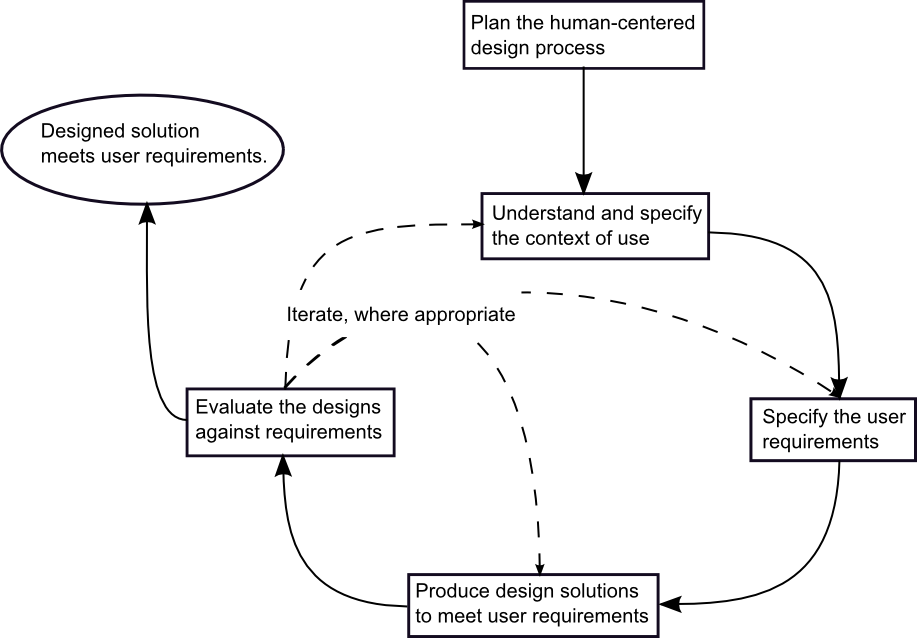
\includegraphics[width=0.9\textwidth]{hcdActivities.png}
		\caption{\footnotesize The human-centred design workflow}
		\label{fig:hcdActivities}
\end{figure}

The standard describes 6 key principles, as listed below. These principals in combination with figure~\ref{fig:hcdActivities} will ensure that the design is user centred. The figure is in no way a strict linear process to follow, it merely shows the required input and expected result of each activity.

\begin{enumerate}
  \item Users are involved throughout design and development.
  \item The design team consists of members with varied backgrounds
  \item The design is based upon an understanding of users, tasks and environments.
  \item The design is driven and refined by user centred evaluation.
  \item The process iterative.
  \item The design addresses the whole user experience.
\end{enumerate}

The first principle emphasizes user involvement throughout the entire process, and not just at the start and the end of the system design, but through the entire cycle of activities. It is important to include a wide range of views and input from experts in various fields, this is where the second principle comes in. It ensures that not everyone thinks and approaches the problem in the same way. The third principle involves understanding the user, what they want to do with the system, and the environment the system will be used in, this is sometimes referred to as the \textit{user experience trinity}. 

Principle 4 and 5 address the fact that several iterations might be required for a satisfactory design to be reached. Users might not know what they want, but they do know what they do not want once they have experienced it. Multiple iterations and examples may then be required to find something that is satisfactory to the user. The final principle states that the usability is not just about making things easy to use, but provide the user with a emotional and perceptive stimuli as well. They should wish to use the system and feel good about it.

\section{Information Visualization}
%DENNE SEKSJONEN TRENGER FLERE BILDER FOR � ILLUSTRERE POENGET V�RT.SJEKK https://www.interaction-design.org/ UNDER DATA DOCUMENTS, VI KAN OGS� BRUKE BILDER FRA D3JS.
Information visualization is useful when you want to display large amounts of data simultaneously. The human brain is not good at getting an overview of the information by looking at large tables of numbers or text. Visualizations utilize the strengths of human cognition. By using computer graphics to make visualizations, large amounts of information can be displayed in a way that humans can process and analyse quickly and intuitively.

Many guidelines have been suggested for creation of the optimal visualization. Shneiderman summarized many of these principles in his \emph{visual-information-seeking mantra}~\cite{shneiderman}:

\vspace{-13pt}
\begin{quote}
\textit{Overview first, zoom and filter, then details on demand.}
\end{quote}

For the visualization to be effective the user has to get an overview of how the information is presented. The system should also allow for zooming in on interesting parts of the information as well as giving the opportunity to filter out information that is not of interest. Most visualizations remove some level of detail for the data to be more accessible and easier to read. Therefore it is important that the system allows the user to access more detailed data when needed.

Shneiderman also identifies the importance of showing the relationships between different items, allowing the user to extract subcollections of the displayed items and storing the user action history to allow for undo/redo functionality.

\subsection{Visual Variables} 
// This section needs descriptive illustrations, see www.interactin-design.org (article at the bottom).

One important factor to consider when creating a visualizations are which visual variables to use. To create an intuitive visualization it is important use the different visual variables correctly. We will briefly go through some of the more common visual variables here and discuss how and how not to use them, based on Carpendales article about the subject~\cite{carpendale}.

\textbf{Visual variables:}
\begin{table}[h!]
  \begin{tabular}{|l|p{10cm}|}
      \hline
      Position    & Position of object, for example x- and y-coordinates in a two dimensional system. \\ \hline
      Size        & Size of object. \\ \hline
      Value       & Change in colour scale from light to dark. \\ \hline
      Colour      & Change hue for given value, for example blue, red and yellow. \\ \hline
  \end{tabular}
  \caption{Overview of visual variables.}
\end{table}

\textbf{Characteristics of visual variables:}
\begin{table}[h!]
  \begin{tabular}{|l|p{10cm}|}
      \hline
      Selective   & Will a change in this variable make it easier to select it from a group of variables? \\ \hline
        Associative & Will changes in variables make us able to distinguish different groups of variables \\ \hline 
        Qualitative & Can the visual variable be used to illustrate the numerical value and relationship between variables? \\ \hline
        Order       & Will changes in the visual variable allow us to order them? \\ \hline
        Length      & How many changes is it possible to distinguish between for this type of variable? \\ \hline
    \end{tabular}
    \caption{Description of characteristics of visual variables}
\end{table}

Position fulfils all the characteristics of visual variables. When thinking of a scatter plot it is easy to see that positioning the points will make them selective and associative. By using scales, position can be used to show the value of the variable in a numerical sense, so it is also quantitative. Order is also fulfilled, a ruler is a simple example of how position can be used to order. The length is theoretically infinite, and only restricted by the screen resolution.

Size fulfils all of the characteristics. It is both selective and associative, humans can easily identify for example the smallest circle in a group of circles. Though size can be used to visualize a numerical value, it is often hard for humans to accurately see how much larger one object is compared to another. Different sizes can easily be ordered. As for the length of this variable Carpendale suggest about five different sizes for selection and about 20 different sizes for distinction. It is important to note that humans can identify small changes in size when objects are close, however when the distance between objects is increased it is hard to distinguish between these differences.

Value can be used both for selection and association. Humans can identify darker parts and group them with ease. It is not quantitative, it is difficult to identify that one tone of grey is twice as dark as another. One can however say that one grey tone is darker than another, and therefore you can order them. Carpendale suggest that the length of this variable is less than 7 for selection, and about 10 for distinction.

Colours are selective and associative. Unless you are colour blind you can easily identify and group different colours. Colours are not quantitative, it is hard for humans to say that one colours is twice that of another. Though we have colour scales, humans do not intuitively order colours, this can easily be illustrated by a question: Which colours is greater blue or yellow? Most people will not have an answer. Carpendale suggests that you use less than 7 different colours for selection, and about 10 for distinction.

\subsection{Interactivity}
One of the benefits of creating visualizations for computers is the ability to add interactivity. Shneidermann mentions 6 tasks that should be implemented when creating information visualizations:
\vspace{-3mm}
\begin{description}[itemsep=0cm, parsep=0cm]
  \item[Overview] Show an overview of the entire data set
  \item[Zoom] Let the user look closer at elements of interest
  \item[Filter] The user should be able to filter out tasks that are not interesting
  \item[Details-on-demand] Show details when elements are selected
  \item[History] Let the user undo or redo actions
  \item[Extract] Allow the user to extract a subset of the entire data set
\end{description}

The first thing the users sees when interacting with an information visualization is an overview of the data set. This can be done by zooming out and then let the user zoom in on areas of interest. Another approach is to aggregate the data in separate sections that can then be investigated further.

It is rare that the user is equally interested in every part of the data set, therefore it is useful to be able to zoom in on elements for a more detailed look. It is important to make sure that the user does not loose their sense of position and get lost in the visualization.

Often the some of the data in the set is not relevant and only distorts the visualization. In such cases one should be able to filter out those elements. The user should be able to filter out unwanted data using sliders, buttons etc. The update should happen real-time, to allow the user to see how the filter affects the visualization. 

Typically information visualizations hide the numerical data (or other detailed data) behind the element. It is therefore paramount to give the user the ability to access this data when it is needed. The user should be able to select an element or a small group of elements and browse the details in a list or other textual representation.

When working with a visualizations where you can make changes to filter, zoom, etc. It is useful for the user to be able to undo and redo tasks. Undo will give the user the ability to go back form an undesired zoom level or filter setting quickly. Users will often times do make more actions than they can keep track of, so giving them the ability to trace their steps improves usability.

When the user has used the visualization and found what he was looking for, the user should be able to extract those elements. The extracted elements should be saved in a format that can be sent to and seen by others. 

\section{Interview}
By performing an interview the interviewer wishes to acquire knowledge from the subject (interviewee) through a conversation. Interviews can be unstructured, semi-structured or structured~\cite{interactionDesign}.
\begin{description}
  \item[Unstructured interviews] are exploratory conversations around a certain topic or area of concern. These can be completely informally.
  \item[Semi-structured interviews] follow a general guideline or script that serve as a checklist and provide consistency between interviews. The order and wording can be freely modified to follow the conversation flow, and unplanned follow up questions are often asked.
  \item[Structured interviews] have set of predefined questions with fixed wording and are in a pre-set order. It is much like a questionnaire but allows for slightly more open-response questions.
\end{description}
Ideal structure choice for an interview is decided by its purpose, what questions need to be addressed and how far has development come? If the goal is to gain first impressions, initial design ideas or information about a particular topic then unstructured interviews are often the best approach. A more structured approach is useful when the goal is to get feedback on particular design features such as the layout of a website, in such cases  structured interviews or semi-structured interviews are useful.

% REVIEW: You can mention that interviews are less prone to have problems with the subjects not understanding the question, because the interviewer can explain the questions and what was meant.
The advantage with interviews is that they are flexible and easy to alter prior or during an interview session. The interviewer gets an immediate response from the subject, and can change accordingly if the interview is not working as planned. Interviews do have drawbacks, conducting and transcribing interviews are both time a time consuming process. Bias might also be presents where the subject being interviewed says things he believes the interviewer wants to be hear or neglects to provide information. This might particularly be the case when the interview has gone on for too long and the participant wants it to end \cite{realWorldResearch}.

\section{Brainstorming}
Brainstorming is a generic technique used to generate, develop and refine ideas, it is widely used in interactive design to generate alternative designs and provide better ideas for certain problems~\cite{interactionDesign}. The technique has no real structure or rules, but in addition to the list below \textit{Interaction Design: Beyond Human-Computer Interaction} mentions two key success factors: Participants should know the user goals that the system is intended to support, and that no ideas should be criticized or debated, everything is initially accepted.


\begin{enumerate}
  \item Participants should ideally be from a wide range of disciplines and have a broad range of experience.
  \item Do not exclude unconventional ideas, these can often be turned into useful requirements.
  \item Build one idea on top of another. Suggest jumping back to an earlier an idea if the vigour diminishes. Use a random word from the dictionary and related it to the product if stuck.
  \item Keep records without censoring, and number them so jumping back to previous ideas is easy. Participants should be encoraged to sketch, create diagrams, and keep notes.
  \item Staying focused is important. Having a well articulated and honed problem helps focus people and direct the session back on topic if it wanders.
  \item If the participants are unfamiliar with each other it is important to have warm up exercises such as word games or exploring physical objects available to them.
\end{enumerate}

\section{Prototyping}
A prototype is a realization of a design that stakeholders can interact with and explore. The limitation of a prototype is that it often only focuses on one product characteristic and neglects the others. A prototype can be anything from a complex piece of software to a simple storyboard or sketch. Prototypes serve as an aid by clarifying communication between team members, and efficiently exploring design ideas with stakeholders and designers. Building the prototype itself encourages reflection of the design and is recognized by designers from many disciplines as an important aspect of the design process \cite{interactionDesign}.

\subsection{Low-fidelity vs. High fidelity}
Low-fidelty prototypes do not resemble the finish product very much. It often uses completely different and much cheaper materials then the final product making them cheap, simple and easily modifiable. Examples of such prototypes are storyboards, sketching, and wizard of Oz. Low-fidelity are important in early development stages because the simplicity encourages exploration and modification. The disadvantage is that these prototypes are never kept or integrated into the final product.

High-fidelity prototypes are much closer to the final product, and therefore give a much stronger impression of the final product. The high-fidelity prototype is useful for identifying technical issues and selling ideas to people. These prototypes are often reused or developed into a final product, but require more time and resources to create.

The very nature of a prototype involves making compromises. Therefore the choice of prototype lies in what kind of of questions we want to answer. Two common compromises that are often traded against each other are breadth of functionality vs depth of functionality. \textit{Horizontal prototyping} focuses on a wide range of functions but little details and \textit{vertical prototyping} focuses on providing a lot of detail for a few functions. 

\subsection{What do prototypes prototype?}
In the article \textit{What do Prototypes Prototype}~\cite{prototypesPrototype} Houde and Hill discuss how prototypes need to be designed to test or rather prototype a certain design aspect of the final product. The model shown in Figure~\ref{fig:hillTriangle} represents a three dimensional space which corresponds to important design aspects of an interactive system. Each corner of the triangle represents a set of questions which are essential to the design of a system. \textit{Look and feel} covers questions that concern itself on what the user feels, sees and hears when using the system, in other words the sensory experience. \textit{Role} as the name states refers to questions about what role the system has in the users life, what function does it server and how is it useful to them. \textit{Implementation} addressed the technical aspects of the system, what techniques and components are should be used for it to be able to perform the intended function. The triangle is intentionally skewed to emphasize that no set of questions is more important than the other.
%WRITE ABOUT HOUD AND HILLS TRIANGLE OF AWESOMNESS http://hci.stanford.edu/courses/cs247/2012/readings/WhatDoPrototypesPrototype.pdf

\begin{figure}[h!]
	\centering
		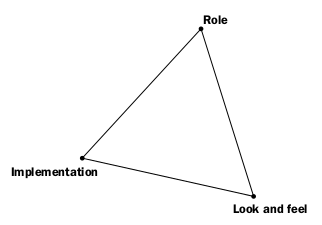
\includegraphics[width=0.6\textwidth]{hillTriangle.png}
		\caption{\footnotesize The prototype triangle by Houde and Hill~\cite{prototypesPrototype}}
		\label{fig:hillTriangle}
\end{figure}

The purpose of the model is to help designers seperate design issues into the three aforementioned set of questions, which often require very different approaches to prototyping. Look and feel requires the user experience to be created or simulated, implementation requires a running system to be built, and role involves researching the use context for the system. Categorizing the important design questions will help decide on what kind of prototype should be built and focus the exploration.

\section{Focus groups}
Focus group, or group interview is an informal technique that can help software developers identify the users needs and feelings about a system. The technique can be used both before interface design and long after the system has been implemented. 

According to Nielsen~\cite{focusGroup} the focus group should have at least six participant to maintain a flowing discussion and provide different perspectives. The participants should be representative of the intended users, or be the final users themselves. Sessions normally last two hours and are run by a moderator. The moderators job is to keep the discussion flowing and let everyone get their point across. Moderators can also guide the discussion in the direction relevant to the goals of the focus groups. 

A single session may not be representative enough or can get sidetracked, it is therefore important to run more than one focus group. If improvements suggested by participants have been implemented it is important to run another iteration of the focus group with the same participants to attain feedback on the changes that have been made. Enough focus groups have been conducted when new information is no longer being received, i.e. a point of saturation has been reached~\cite{howFocusGroup}. 

Nielsen~\cite{focusGroup} discusses two pitfalls with focus groups: Because sessions are in groups the users do not test the system themselves, instead they are presented with a demo. The problem with such a demo is that the participants never have to question what to do next or consider the meaning of the screen options. The second problem is that what participants say they want, is not necessarily what they need. Also, ideas described by the moderator might be perceived differently by the participants. By providing concrete examples through prototypes of the technology, one can minimize this problem.

\section{Questionnaire}
Questionnaires are a research tool that consist of a series of questions with the goal to attain information from the respondent. It is a well established technique for collecting demographic data and user opinion, they are similar to an interview in the fact that they can contain both closed and open ended questions. Clear unambiguous questions and allowing efficient data collection is important, especially if a large quantity of questionnaires have been issued. Questionnaires can be used on their own or as an addition to other methods in order to gain background information, or deepen understanding of a particular topic. Below is a short and general guideline provided by~\cite{interactionDesign} on things to watch our for when creating questionnaires.

\begin{itemize}
  \item The order of which questions appear is important, it can influence the impact of a question.
  \item Consider having alternate versions of the questionnaire to suit different populations.
  \item Clear instructions on how the questionnaire should be filled in essential. Clear wording and good typography is important.
  \item Balance must be attained between whitespace and needing to keep the questionnaire as short as possible. Long questionnaires cost more, and might deter people from participating.
\end{itemize}

The advantage with questionnaires is that hey provide relatively simple and forward study, and may be adapted to collect generalized information from almost any human population which means high amounts of data standardization. If the survey is anonymous it can encourage more honesty then another research method would have if sensitive topics are involved. In addition to being relatively cheap to perform compared to the amount of data that is gathered. There are downsides this form of data collection, people might respond in a way that puts them in a good light, and data is affected by the respondents characteristics. Their memory, knowledge, experience and motivation influence how they answer the survey. A downside with questionnaires without any kind of monitoring are ambiguity or misunderstanding in the survey questions that is never detected, respondents might not take the questionnaire seriously, or there are low response rates.

\section{Validity}
According to \textit{Interaction Design: beyond human-computer interaction} validity is concerned with whether the evaluation method measures what it is intended to measure. This applies to both the method itself and the way it is executed. For example, if one wishes to examine how a product is used in the home, setting up a controlled lab experiment would hurt the validity. Wrong choice of method and execution are not the only threats to validity, bias and the Ecological Validity threaten the validity but can be impossible or hard to avoid.

Ecological Validity is concerned with how the evaluation method and environment themselves influence and affect the results. If a subject is aware of being observed and the test is conducted outside of their natural surroundings their behaviour and answers will be influenced. Bias is when the results are distorted by the researchers and evaluators. Evaluators might fail to note certain behaviour because they deem it irrelevant, or an interviewers tone of voice may influence the answers of the interviewee. It is therefore important to be open to the possibility of bias.

Validity in \gls{hci} is a complex area and we have only mentioned some of the basic issues. Thimbleby reviews some of the more complex issues and suggests some practical recommendations for solving them in his \textit{Validity and Cross-Validity in HCI Publications} paper \cite{validation}. One of the simpler suggestion he makes is to use Triangulation. Triangulation involves using multiple methods or sources to achieve the same result. A more elaborate method to assure good validity involves creating a universal star rating system, where papers should be rated based on how easily a researcher can reproduce or build upon the original work.


\chapter{Physical Therapy for Senior Citizens}
This chapter presents the physical activity and health situation both nationally and internationally, in addition to presenting the Norwegian recommendations for physical activity. It then covers physical therapy in Norway and looks at how sensor technology can be of a help in the field.

\section{Physical activity and health}
In 2010 one of the largest ever systematic efforts to describe the global health situation was conducted. The article was later published in The Lancet~\cite{globalBurden}. One of their many findings was that since 1970 men and women have gained an additional ten years to their life expectancy, but spend more time living with injuries and illness. 

The amount of time adults spend in a sedentary position has increased over the last 30 years. The reasons for this are many, but increased use of technology and ease of transport are one of the main factors~\cite{sedentaryBehaviour}. An American study shows that 1 of 4 US adults spend 70\% of their waking hours in a sedentary position, 30\% in light activity, and little to no time is spent exercising. During the last decade research has started to emerge that links extended periods of sedentary time to metabolic risks~\cite{sedentaryTime}, obesity, and abnormal glucose metabolism~\cite{breaksSedentary}. It is suggested that prolonged periods of sedentary time should be avoided by increasing the number of breaks during sedentary time. 

Based on these findings health recommendations regarding breaks in sedentary time should be added to the already existing ones~\cite{breaksSedentary}. Another study goes as far as stating that prolonged sedentary time is strongly related to metabolic risks independent of physical activity~\cite{sedentaryActivity}, and that elderly benefit more from reducing time spent sedentary than younger people. Though researchers agree that long periods of sedentary time is unhealthy, research still has to be done on how long a subject can stay sedentary before it has negative impact on the individuals health. How long you need to stay active between periods of sedentary time is also debated.

The \gls{ndh} has issued recommendations and guidelines pertaining to the minimum amount of physical activity for en elderly person. The recommendation is set to a minimum of 30 minutes a day with moderate activity~\cite{helsedirektoratetFysiskAktivitet}. In addition to this an elderly person should be standing in a skeleton bearing position for total of 5 hours per day to preserve the skeletons strength and form. Skeleton bearing position means that the subject is standing upright without any aid, such as a walking stick.

\section{Physical Therapy in Norway}
Physical therapy consists of two main steps: diagnosis and treatment. In the diagnosis phase the physiotherapist tries to determine what is wrong with the patient in order to apply the appropriate treatment. In case of elderly patients their problems might often be caused by lack of activity. When the therapist is finished with the diagnosis, a treatment plan is created. The plan is typically a set of exercises the patient should preform throughout the week. The plan is designed to let the patient reach his goals regarding activity.

The treatment phase consists of the patients following the agreed upon plan to improve their activity level or regain normal movement after operations or fractures. At a future time the physiotherapist will return to the patient to monitor the progress of the patient. Often the patient may lack the dedication or motivation needed to follow the plan strictly. In such cases the plan might need to be revised or the physiotherapist needs to perform checkups more often to ensure that patient stays motivated.

\section{Sensor Technology in Physical Therapy}
There is no use of sensor technology to track activity in Norway today. Some of the physiotherapists we have been in contact with worked on research projects where such technology was utilized, but they had never used it outside of academic work.

Even though there is little use of this type of technology in physical therapy today, the Norwegian government has an increasing focus on the use of welfare technology. A committee formed by the Norwegian government called \gls{hu}~\cite{haagen} also concluded that there is a need for more welfare technology to tackle the ever increasing number of elderly. A system that could increase the effectiveness and quality of physiotherapist's work toward activating the elder population fits well with the technological goals presented in the \gls{hu}-report.  

\section{Potential of Accelerometer}
Using accelerometer data to classify activity can help both in the diagnosis and treatment phase. Having quantitative data of the users activity over one or more weeks, will give physiotherapists a much better overview of the patients current activity level. This can be helpful when creating a treatment plan.

Letting the patient see their improvement using information visualization can be a powerful tool in motivating the patient. Sometimes the improvement might be subtle and it can be hard for the patient to be motivated to continue the exercise plan without seeing some kind of indicator that they are in fact improving. Patients also tend to trust in statistical data, because it is quantitative. 

%\section{Medical Technology}

%In 2006 the Norwegian government announced a regulation concerning medical equipment. The purpose of the regulation is to ensure that medical equipment used in Norway does not present a danger to either patient or users. To insure this, the regulation instils a set of requirements to both the use and the production of the equipment. In the regulations definition of medical equipment standalone software is also to be perceived as medical equipment. This means that the system created in this project would need to be pass the regulations requirements before such software could be used in practice. 

\chapter{Body-worn Sensor Technology}
The purpose of this chapter is to give an insight into relevant commercial products that exist today. It starts off by looking at the communities that surround these products before presenting the technology itself. Finally we discuss and display how these products present their activity data.

\section{Personal Informatics and Quantified Self}
Currently there are two names that stand out within the self-monitoring field: \gls{qs} \cite{quantifiedSelf}, and Personal Informatics (PI) \cite{personalInformatics}. \gls{qs} is a community of end-users who share data and exchange experiences with tools that help them collect information. \gls{pi} is a label used to classify a set of tools used for self monitoring. \gls{pi} also refers to a community that hosts conferences concerning research in the field of \gls{pi}.

\subsection{Personal Informatics}
Personal informatics is the label used to classify tools that help people collect personal information for the purpose of self-monitoring and self reflection. These tools are used to help individuals gain self-knowledge about their behaviour, habits, and thoughts.

The \gls{chi} conference has since 2010 \cite{chi2010} held workshops and accepted papers on Personal Informatics. The aim is to increase the understanding of how the tools affect the users as well as explore new possibilities, and overall improvement of the user experience.

\subsection{Quantified Self}
In 2011 \gls{qs} had their first conference \cite{bodyHackers}. Here people shared data that they had collected about themselves using different types of devices. Members of the community collect information about everything from sleep patterns and diets to mood and stress levels. The goal is to use quantitative data to improve ones own life, either through a more healthy lifestyle or by achieving a better understanding of oneself. 

To promote further development in tools that gather these types of information, the participants of Quantified Self have worked closely with companies and individuals that create personal informatics tools. Devices such as Nike's FuelBand and Fitbit are results of this cooperation, and both products have been well received by the community.

\section{Sensor technology}
% REVIEW: Read and give your judgement.
This section covers some popular commercial activity monitoring sensors currently on the market. The products that will be discussed are Nike Fuelband, Fitbit Flex and activPAL. Both Nike FuelBand and Fitbit Flex are designed for the personal use, while activPAL is manly used in research projects.

\subsection{Wrist-worn Body Sensors}
Since the release of the Nike+ FuelBand~\cite{fuelBand} in early 2012 several new wrist-worn activity monitors have emerged. Nike FuelBand, Fitbit Flex~\cite{flex} and Jawbone Up~\cite{jawboneUp} are the only ones, so far, who are either available to the public or soon to be released. The devices are designed to be inconspicuous, durable and to quietly monitor the users activity by counting steps taken, kilometres walked, time spent sleeping or sedentary etc. All of the bracelets use a built in 3-axis accelerometer to record movement. The classification of activity level is done by individual proprietary algorithms for each of the products.

\begin{figure}[h!]
  \centering
  \begin{subfigure}[b]{0.3\textwidth}
    \centering
    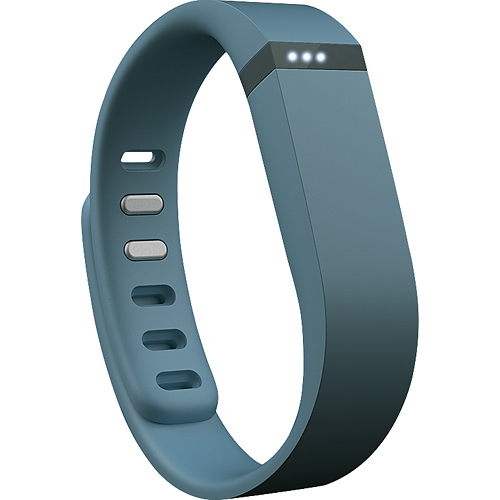
\includegraphics[width=\textwidth]{fitbitFlex.png}
    \caption{Fitbit Flex}
    \label{fig:fitbitFlex}
  \end{subfigure}
  \begin{subfigure}[b]{0.4\textwidth}
    \centering
    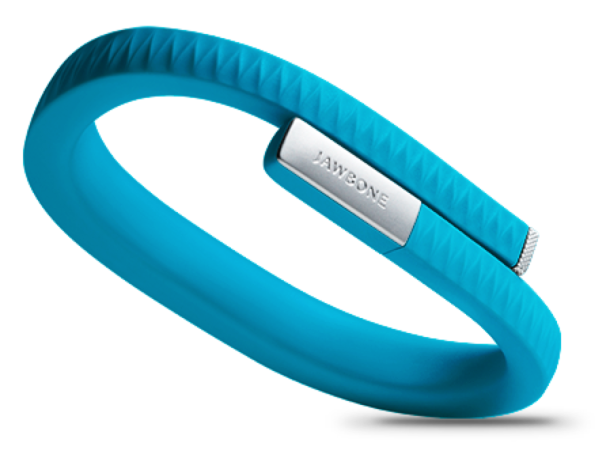
\includegraphics[width=\textwidth]{jawboneUp.png}
    \caption{Jawbone Up}
    \label{fig:jawboneUp}
  \end{subfigure}
  \caption[Fitbit Flex and Jawbone Up]{Two commercial wrist worn body sensors.}
\end{figure}

Being worn on the wrist these devices come with certain drawbacks, all the information gathering is based on movement from a single point (i.e. the users wrist). This leads to certain physical activities not being registered properly, one such example is riding a bike. The Fitbit developers have attempted to compensate for this by allowing the user to track such activity manually. The manually entered data is then added to the daily statistics. 

\subsection{activPAL}
\label{sensorActivPal}
The activPAL sensor has the shape of a small rectangle and is worn on the thigh. When the device is active it continuously records accelerometer data using an internal accelerometer. This data can be interpreted using algorithms provided by PAL Technologies.

\begin{figure}[h!]
	\centering
		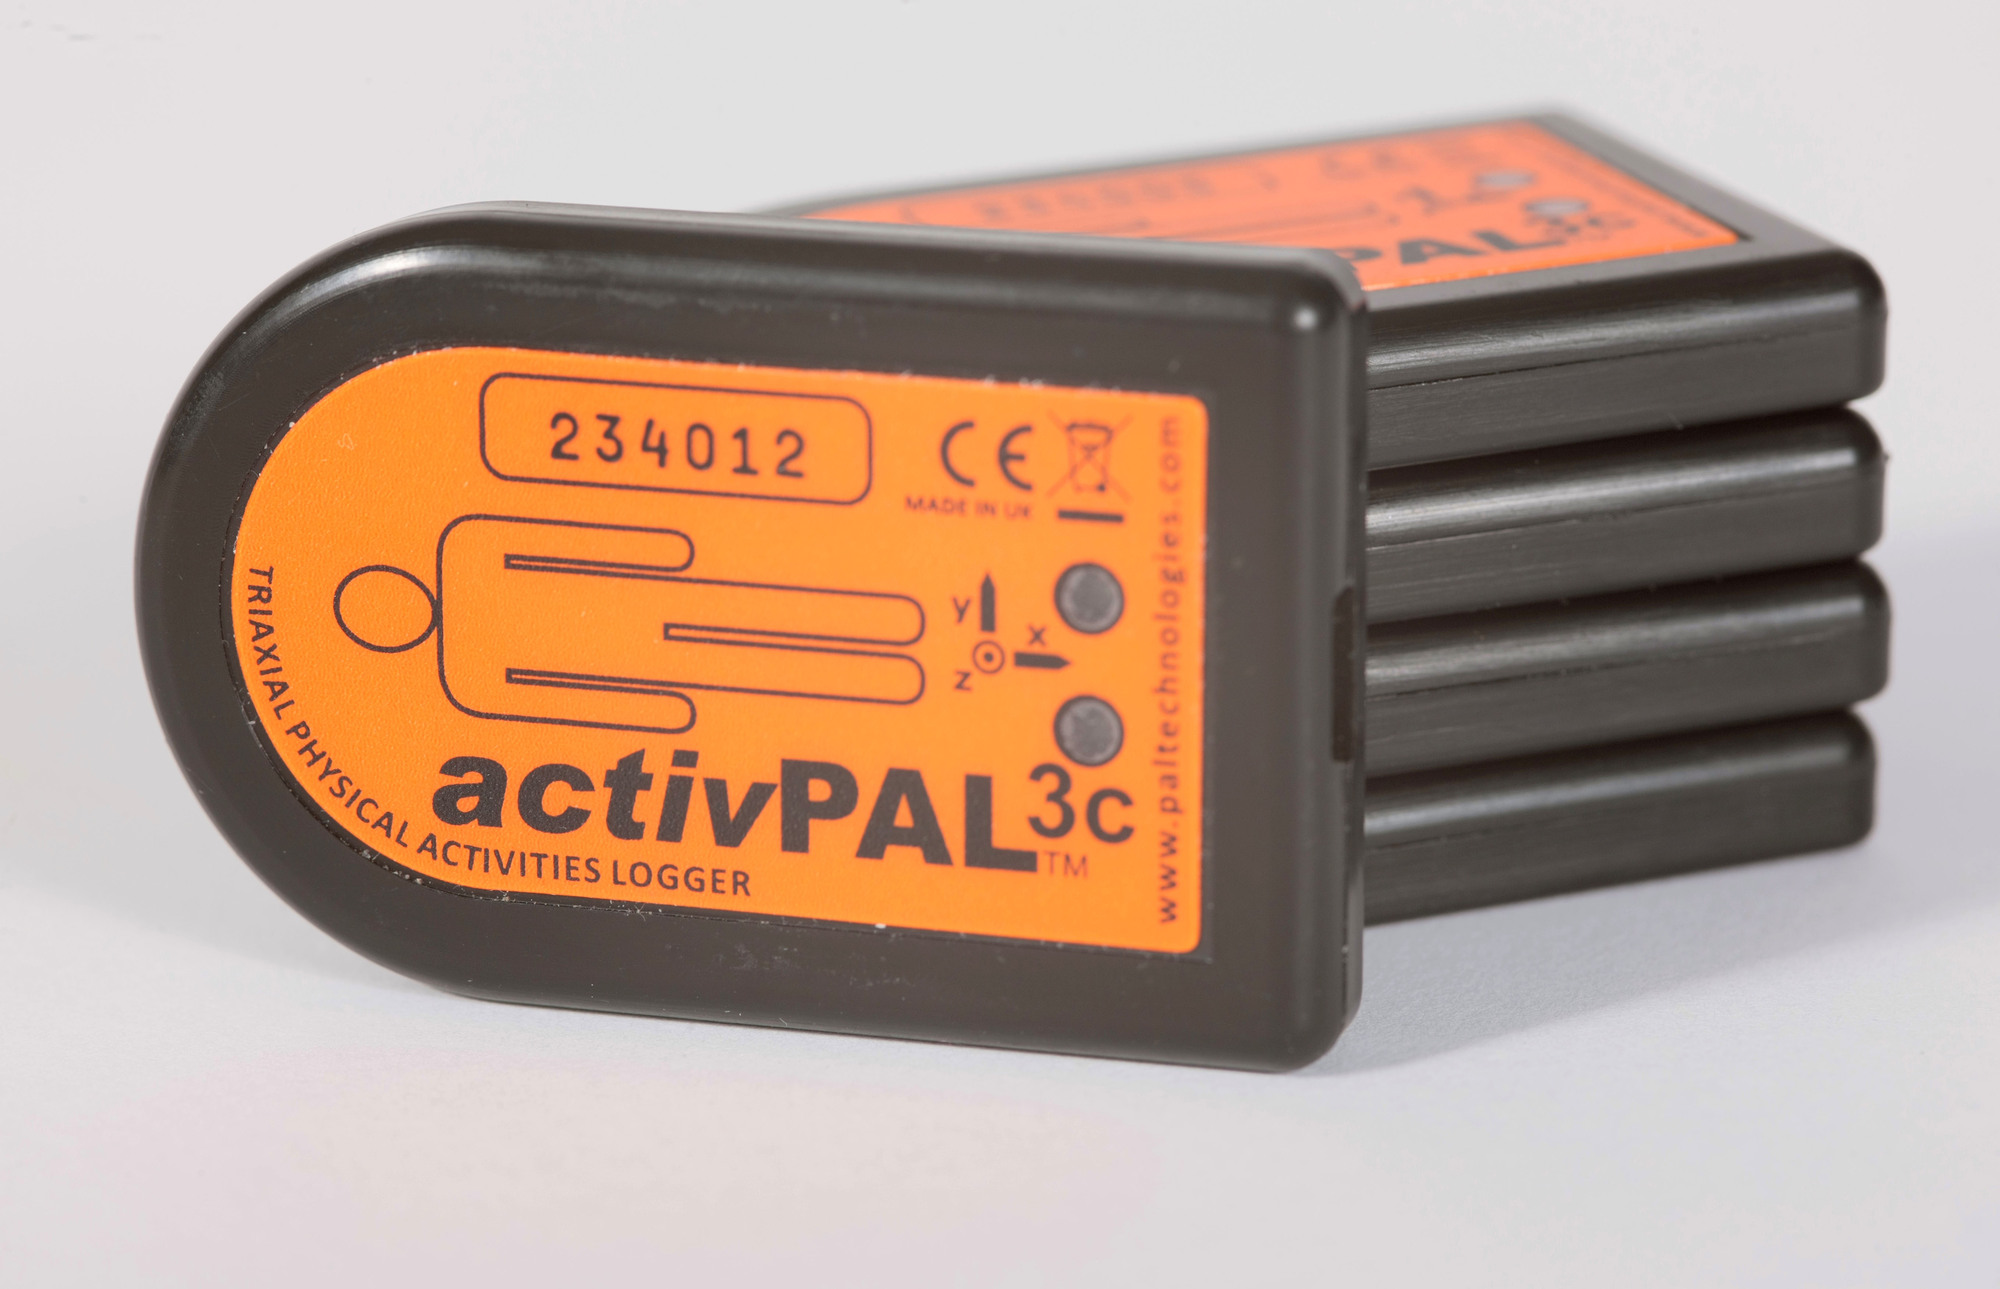
\includegraphics[width=0.6\textwidth]{activPALs.jpg}
		\caption[activPal sensor]{An activPAL tri-axis sensor.}
		\label{fig:activPal}
\end{figure}

When the activity data has been gathered the \emph{Intelligent Activity Classification}-algorithm is used to classify the data into three states: sitting/lying, standing and walking. Because activPAL is worn on the thigh, the accelerometer is unable to detect the difference between sitting and lying. Number of steps is also counted when walking.

% REVIEW ME and next section
activPAL differs from the other sensor presented in this chapter as it is designed for use in research and not commercial use. The sensor has a longer battery life than Fitbit Flex and Nike+ Fuelband, but does not include a practical way to be carried and has to be taped to the thigh. It is also much bigger than Fitbit Flex and Nike FuelBand. 

activPAL is frequently used in research, several studies have been conducted which conclude that the sensor is viable for recording and classifying activity \cite{grant2006, ryan2006, grant2008, tsavourelou}. The sensor has also been used in multiple studies for obtaining and analysing activity patterns~\cite{grant2010, lord, ryan2010}.

\section{Presentation of Sensor Data}
In this section we look at how the commercial activity monitoring devices presented in the previous section visualize their data. We will show that the Nike Fuelband and Fitbit Flex, designed for the general public, have a much broader range of visualizations with greater emphasis of being visually appealing than activPal.

\subsection{Nike+}
NikeFuel \cite{nikefuel} is a unit of measurement used by all Nike's activity trackers. The FuelBand does calculate steps and calories burned, but the NikeFuel is the prime focus of their product line. NikeFuel does not take into account gender, height, weight, but looks purely at activity. Meaning that a kilometer of walking will award the same amount of points to users with very different physiology. The daily progress (Figure \ref{fig:tworings}) is represented through a ring that fills up when the FuelBand detects activity. A full ring means that the daily goal has been reached. Progress beyond the daily goal will be displayed with numbers and visual enchantments on the ring. 


\begin{figure}[h!]
 \centering
  \begin{subfigure}[b]{0.49\textwidth}
    \centering
    \includegraphics[width=0.5\textwidth]{nikering.png}
    \caption{User having one third of his daily NikeFuel goal~\cite{fuelbandDcRain}.}
  \end{subfigure}
  \begin{subfigure}[b]{0.49\textwidth}
    \centering
    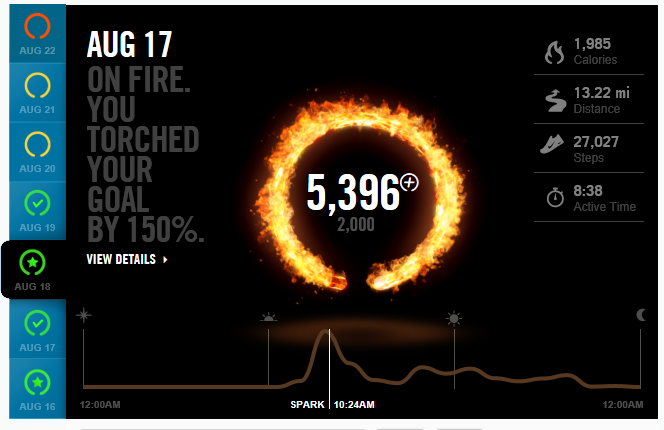
\includegraphics[width=\textwidth]{ringfire.png}
    \caption{User beating his daily limit by 150\%, rewarding him with special effects on the ring~\cite{fuelbandTechSpce}.}
  \end{subfigure} 
  \caption[Nike+ visualisations]{Two examples of Nike+ visualizations.}
  \label{fig:tworings}
\end{figure}

An online profile provides detailed information about the users activity, showing steps, calories burned, active time, distance travelled and average fuel, as seen in Figure~\ref{fig:activityBreakdown}. Charts can be displayed for weeks, months or years. This allows the user to track their progress and look at how often they achieve or exceed their goals~\cite{fuelbandTechSpce}. 

\begin{figure}[h!]
	\centering
		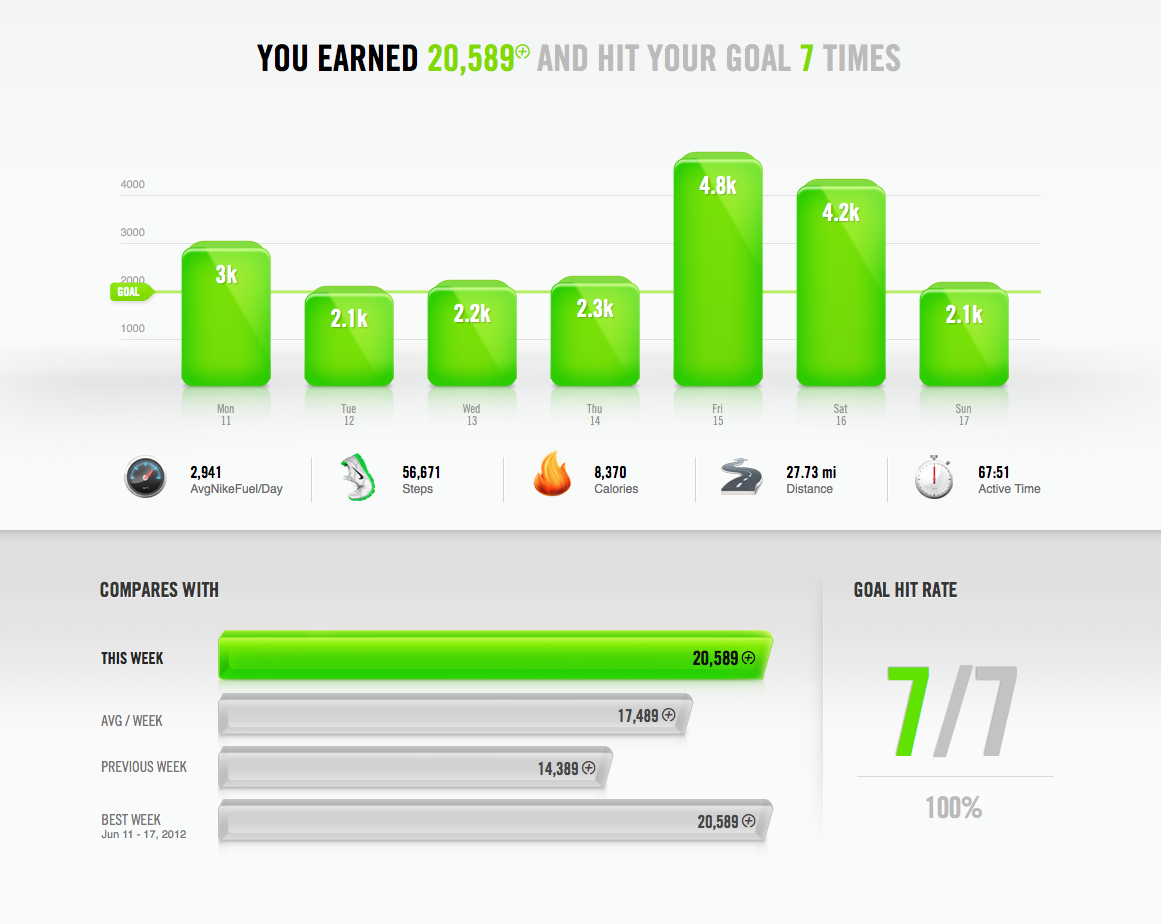
\includegraphics[width=0.7\textwidth]{week.png}
		\caption[Weekly breakdown (Nike)]{The weekly breakdown presented by Nike+. \cite{fuelbandTechSpce}}
		\label{fig:activityBreakdown}
\end{figure}

Virtual trophies are awarded for various achievements such as gathering an x amount of NikeFuel or beating the set goal by a 100\%. These trophies can then be shared with friends or displayed on the public profile to show off achievements. A review has reported that the NikeFuel concept can almost become an addiction and lead to doing some last minute workouts in order to reach the goal~\cite{fuelbandDcRain}.

\subsection{Fitbit}
Similar to the Nike+, Fitbit \cite{fitBit} allows the user to set daily goals, but as the Fitbit does not use the NikeFuel system. Instead it allows the user to set 3 separate goals: steps taken, floors climbed, and calories burned, as seen in Figure~\ref{fig:fitbitActivityBreakdown}. The Fitbit provide an active score, but there is no emphasis on it. On the Fitbit-webpage daily activity breakdown is provided. Activity levels are separated into four categories: sedentary, lightly active, fairly active, and very active. All the goal histories can be viewed on the online profile and can be categorized into day, week, months and years. 

Fitbit also offers the Fitbit Premium service, which adds more functionality to the online webapp. The premium service allows the user to get more detailed and aggregated information than the basic logs do. It gives advice on sleep, activity and food based on activity level and the recommended values for people in the users height, weight, age group.

\begin{figure}[h!]
	\centering
		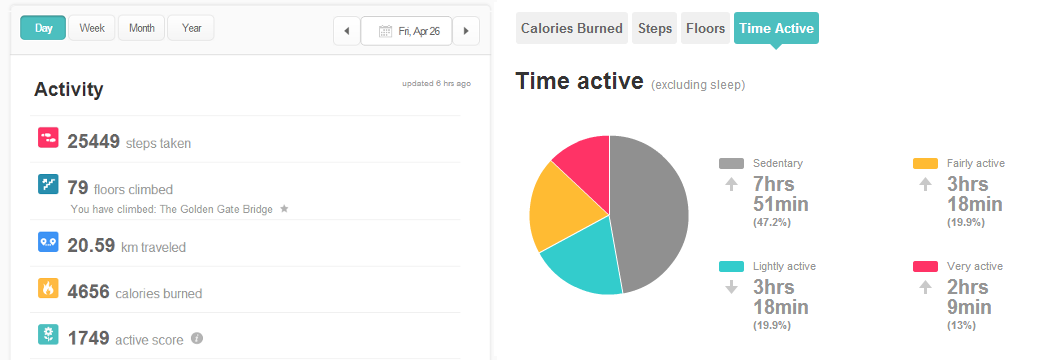
\includegraphics[width=0.9\textwidth]{fitbitActivityBreakdown.png}
		\caption[Fitbit+ visualizations]{The breakdown provided by FitBit. It can be broken into day, week, month, or year.}
		\label{fig:fitbitActivityBreakdown}
\end{figure}

\subsection{activPAL}
\label{sec:activPALViz}
The activPAL only provides one diagram, which can be seen in Figure~\ref{fig:activPalActivityBreakdown}. Yellow represents a sedentary position, green indicates an upright position and red means that the user was walking. If there is activity during an hour, the bar will rise and the activity will be colour coded to either red or green depending on their activity type. Looking at Figure~\ref{fig:activPalActivityBreakdown} we can see that at 10 AM the person spent a long time standing, a little while walking and almost no time was spent in a sedentary position. The pie chart and numbers to the right use the same colour coding and summarizes the activity distribution throughout the day.

\begin{figure}[h!]
	\centering
		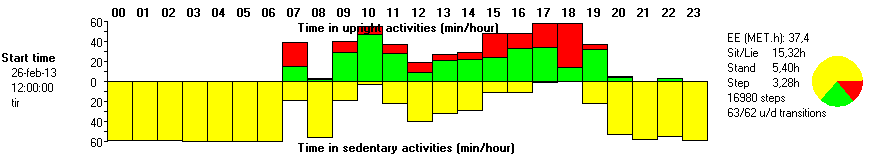
\includegraphics[width=1\textwidth]{activPalChart.png}
		\caption[activPal visualizations]{Visualization of sensor data from activPAL sensor.}
		\label{fig:activPalActivityBreakdown}
\end{figure}

\chapter{Research Design}
\label{ch:researchDesign}
All of our research methods are of a qualitative nature meaning no empirical data is collected. This Chapter provides an overview of our chosen research methods, how they attempt to answer the research questions and discusses why these methods were chosen.

\section{Overall Plan}
\label{sec:overview}
This section provides an overview of how our chosen research methods relate to each other and how they assist in answering the research questions we have posed. Table~\ref{tab:designPlan} gives a quick overview of our methods and which specific research question the method contributes to. The table order corresponds to when in our project the research method was used.

The first research question is concerned with finding relevant scenarios for the use of systems such as the one we are creating. To answer this question we performed interviews and focus groups. A large part of the second focus group was dedicated to discussing different scenarios with the physiotherapists.

The second research question asks what functional and user experience requirements the visualizations should have. The initial requirements were gathered through an interview with a domain expert. Two additional revisions of the requirements were planned, one after each focus group. Feedback on the prototype was the basis for the modifications to the requirements. A portion of the second focus group was used to discuss the requirements with the physiotherapists.

Research question three asks which visualizations the physiotherapists prefer, given the requirements and scenarios created. Feedback on the visualizations was given in the focus groups. The larger part of both focus groups was dedicated to discussing and reviewing the visualizations with the physiotherapists. 

\begin{table}[h!]
  \centering
  \begin{tabular}{|p{0.7cm}|p{2.2cm}|p{8.8cm}|}
    \hline
    \textbf{RQ} & \textbf{Method} & \textbf{Description} \\ \hline
    1,2 & Interview & An interview was performed with a domain expert to establish initial requirements and scenarios. \\ \hline
    2 & Brainstorming & Based on the initial requirements, the authors performed brainstorming sessions among themselves and sketches were created. \\ \hline
    2, 3 & Prototype & The paper sketches were used as a starting point to create a high fidelity prototype that would be presented to the first focus group. \\ \hline
    1,2,3 & Focus group & The first running prototype was presented to the focus group and would enable us to refine it further. \\ \hline
    2, 3 & Prototype & Based on the feedback received from the first focus group the prototype was modified and improved. \\ \hline
    None & Questionnaire & Before the final focus group, a quick questionnaire was answered by the users. \\ \hline
    1,2,3 & Focus Group & The new version of the prototype was presented and the requirements were refined. \\ \hline
    1,2 & Interview & The interview was carried out to help us understand how the physiotherapists work. \\ \hline
  \end{tabular}
  \caption[Overall design plan]{The overall design plan.}
  \label{tab:designPlan}
\end{table}

More detailed information about how the methods were executed and their result can be found in the subsequent chapters of this report, namely in Chapters 6 to 10. The following sections of this chapter explain the rationale and choice of method in further detail.
 
\section{Overall Plan in Accordance to ISO 9241-210}
This section aims to show how our chosen research methods relate to human-centred design activities describes in ISO 9241-210. Figure~\ref{fig:hcdActivitiesOurs} show how our research methods correspond to the ISO activities. The gray text is the purpose of the step described in ISO 9241-210, inside of the squares are our research methods with a numbering showing the order in which they were executed. The brainstorming and questionnaire activities have been omitted from the figure, as they were primarily used as support methods for prototype 1 and focus group 2.

\clearpage

\begin{figure}[t]
	\centering
		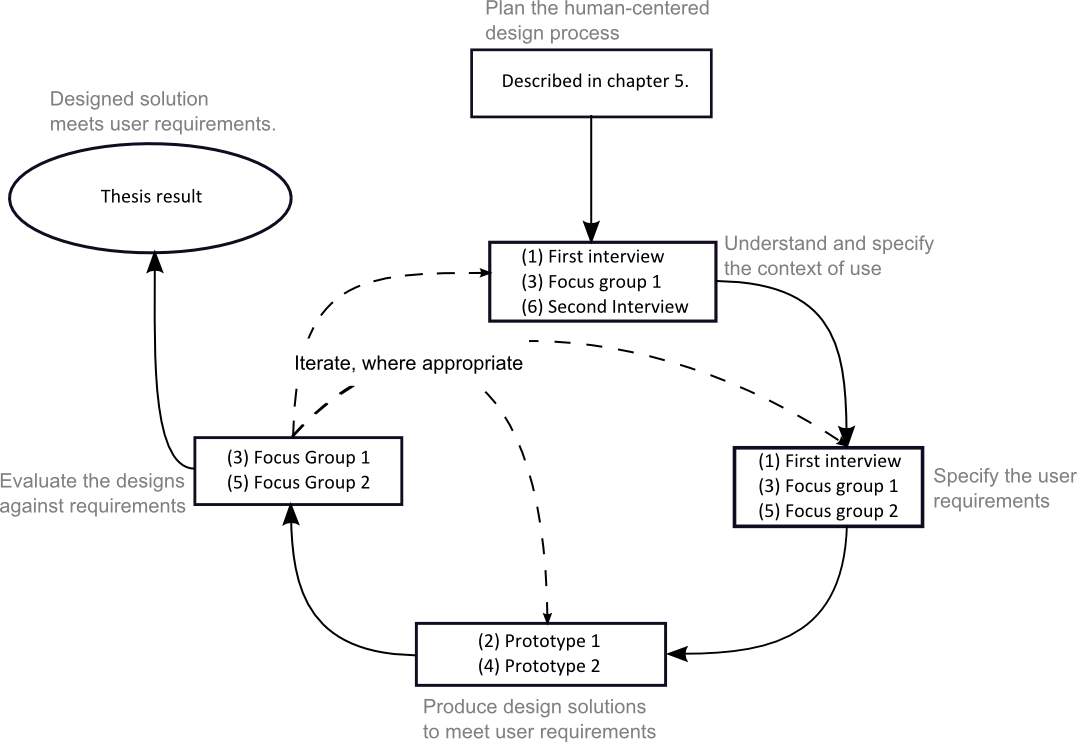
\includegraphics[width=0.9\textwidth]{hcdActivitiesOurs.png}
		\caption[Project workflow]{How our chosen research methods fit into the activities suggested by the ISO}
		\label{fig:hcdActivitiesOurs}
\end{figure}

\section{Interview}
Initially we possessed little domain knowledge on how to create a system for showing visualizations of sensor data to physiotherapists. To increase our knowledge in the field we considered conducting a field study or a focus group, but settled on doing an interview with a domain expert at St. Olav's Hospital. We believed that a field study or focus group would not be fruitful enough to justify the amount of time it would take. We lacked some basic knowledge and terminology in the field, which could be covered by a simple interview. The procedure and results of this interview can be found in Chapter~\ref{ch:initialRequirements}. 

Originally we had intended to conduct a minor literature study to understand how physiotherapy is conducted in Norway. Sadly this was not a well documented process, and the little information we did find was not consistent. The routines varied from office to office, and what type of patients they focused on. Therefore we decided to conduct an interview with some of the participants from the planned focus group. The results of this interview can be found in Section~\ref{sec:physiotherapyPractice}.
 
\section{Brainstorming}
Jumping straight to a high fidelity prototype would be unwise, therefore we decided to conduct brainstorming sessions. The purpose was to create rough designs of possible visualizations that would fulfil the initial requirements, in addition to discussing any technical difficulties that might occur during implementation. The result of the brainstorming can be found in Section~\ref{sec:paperSketches}.

% REVIEW, BITCHES
\section{Prototype}
Implementation of the first prototype was planned to start after the creation of paper sketches. We did not want to spend more time on low fidelity prototypes that would be thrown away at the end, and would most likely never be shown to a broader set of users. A running prototype showing real data and more polished visualizations would have a much bigger impact on the focus group than rough paper sketches. Another important factor was to show the participants of the focus groups visualizations created real-time from actual data. This way they could get an impression of how quick the parsing and rendering was, and how easy it was to switch between patients data. The first version of the prototype can be seen in Section~\ref{sec:runningPrototype1} and the second version can be found in Section~\ref{sec:runningPrototype2}.

Figure~\ref{fig:hillTrianglePrototypex} shows what type of design questions the paper sketches and running prototypes attempt to answer (see Section~\ref{sec:prototypesPrototype}). The Paper sketches (PS) are a result of the brainstorming session conducted. They focus heavily on \textit{look and feel}, as they were designed with the scenarios and requirements in mind, but some \textit{role} questions are answered as well. Our first running prototype resolved any implementation uncertainties we had, and in addition helped us solidify our look and feel. Creating the second prototype after a focus group allowed us to refine the look and feel, as well as focusing more on the roles by using the feedback and comments from the focus group session.

\clearpage

\begin{figure}[t]
	\centering
		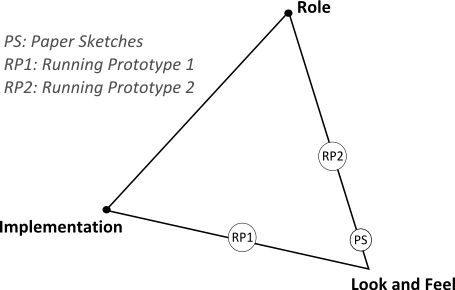
\includegraphics[width=0.7\textwidth]{hillTrianglePrototypes.png}
		\caption[Prototype focus]{Showing where the focus of our prototypes lie.}
		\label{fig:hillTrianglePrototypex}
\end{figure}

\section{Focus Group}
We considered performing usability tests instead of focus groups to get feedback on the system. In the end we decided to conduct focus groups because the main priority was to evaluate the visualizations and not the application as a whole. Usability test focus more on navigating and completing tasks in a system, which is not the focus of this study. Focus groups are also less time consuming and gives the participants the ability to discuss different parts of the system and suggest new features and improvements. We can also use the focus groups to discuss other topics such as scenarios and requirements. Detailed information on how the first focus group was conducted and its results can be found in Chapter~\ref{ch:focusGroup1} while the second focus group is covered in Chapter~\ref{ch:focusGroup2}.

\section{Questionnaire}
A questionnaire was prepared for the second focus group. The purpose was to gain background information about the participants, and to gain an understanding of their attitude towards technology. The questionnaire also asked the participants if they thought using technology such as the one presented in the focus group would improve the quality and effectiveness of their work. The questionnaire was answered at the start of the second focus group. The information received from it is summarized in Section~\ref{sec:participants}

\chapter{Initial Requirements}
\label{ch:initialRequirements}
%Review me!
This chapter presents the interview we conducted which would lead to the creation of our initial scenarios and requirements for our research questions. The first section introduced the participants and the topics that were discussed. The following section presents the interview results, scenarios, and initial requirements.

\section{Participant and Process}
\label{sec:reqGathering}
The initial requirements were gathered with the help of a female domain expert with a Master of Science in Human Movement Science. She is working on a research project at St. Olavs Hospital for her PhD, where the activPAL sensor is used to track the activity of patients being rehabilitated after hip-fractures.

Because of the lack of information we had on the current usage of sensor technology in physiotherapy and how this technology works, we conducted an unstructured interview with the domain expert. In the interview we discussed four topics: how sensor technology like the activePAL is used in physiotherapy and research today, what types of visualizations are used, technical aspects of using the activPAL, and initial requirements. 

\section{Results}
Currently there is little or no use of sensor technology in physiotherapy. There are some physiotherapists involved in the research projects using these types of sensors, but they do not use them in their normal practice. 

The only visualization utilized by the domain expert and physiotherapists using the activPAL sensor are the visualizations that are offered by the software that comes with the sensor, as seen in section~\ref{sec:activPALViz}.

From a technical aspect it is not hard to use the data gathered by activPAL. The data can easily be exported in the common CSV format. CSV is a machine-readable format, which means that can easily be read and parsed by other computer programs. activPAL offers options for exporting both event data (see appendix~\ref{csvDocument}), or raw acceleration data.

After getting an overview, of the current situation and the technical possibilities of the activPAL sensor, we created the initial requirements found in the next subsection.

\subsection{Initial Requirements and User Scenario}
After talking to the domain experts at St. Olavs Hospital, two main user scenarios emerged:

\begin{table}[!h]
  \centering
  \begin{tabular}{|c|l|}
    \hline
    \textbf{Id} & \textbf{Scenario} \\ \hline
    IS-1 & Mapping the activity level of patients \\ \hline
    IS-2 & In consultation with patients \\ \hline
  \end{tabular}
  \caption{Table of the initial scenarios.}
\end{table}

The current practice of physiotherapists working with the elderly is to first get an overview of the patient's activity level. This information is then used to create a program to improve the activity level of the patient. The activPAL sensor can be used in addition to current techniques to gather more quantitative data to get an even better mapping of the patients level of activity. Scenario 1 is concerned with how to visualize this data so that the physiotherapists quickly can get an idea on how to proceed with the treatment.

After the physiotherapists has an idea of the patients current level of activity the data is presented to the patient. This is usually a discussion about the results of the test and what the patient wants to achieve in terms increased activity. Scenario 2 deals with how the visualizations can be helpful in making the patient understand and becoming aware of the current level of activity.

Using the two user scenarios above we created some simple requirements for the visualizations as a basis before starting development.

\begin{table}[h!]
  \begin{center}
  \begin{tabular}{|c|p{12cm}|}
    \hline
      \textbf{Id} & \textbf{Requirement} \\ \hline
    \multicolumn{2}{|l|}{The visualizations should \ldots} \\ \hline
      IR-1 & give an overview of the week \\ \hline
      IR-2 & give a summary of the daily activity \\ \hline
      IR-3 & show the activity level for each hour of every day \\ \hline
      IR-4 & let you compare hours from multiple days \\ \hline
      IR-5 & show the activity level for each minute of every day \\ \hline
      IR-6 & let you compare minutes from multiple days \\ \hline
      IR-7 & let the user identify patients that are active during the night \\ \hline
  \end{tabular}
  \end{center}
  \caption{Table of the initial requirements.} 
\end{table}

\chapter{Prototype 1}

\section{activPAL}
%Synes vi burde vise et eksempel av csv fila, og kanskje bare forklare veldig kort, men siden det egentlig ikke er oppgaven føler jeg at det hører til i appendix.
As mentioned in Section~\ref{sensorActivPal} the activPAL classifies the accelerometer data into 3 different types of behaviour, this data can then be viewed through activPALs proprietary software. There is an alternative to export the data in a \gls{csv} format, and there are several options as how the data should be presented or aggregated. It is possible to display raw accelerometer data or provide event based data where a new entry is created if the state has changed. A new line will then be written with the time, duration and state type every time the state changes. A more detailed overview of the \gls{csv} file can be found in (REF TO APENDIX)

For the purpose of our thesis the event based \gls{csv} was the most suited basis for the type of information we would need for our visualizations. Before feeding the data to our visualizations the applications parsed the data into a suitable format, this primarily consisted of merging all the events into hours and days. activPAL is not vital part of our prototype, instead it was a sensor that was available to us and has been proven trustworthy in other research. Other sensor can be used as long as the data given as input to the visualizations has a certain structure.



\section{Paper sketches}
All the sketches described in this section were created through a set of informal brainstorming sessions between the authors where we occasionally received input from other sources. This was an iterative process that spanned over five sessions. The sketches represent our first ideas on visualizations that would fulfil the initial requirements efficiently, while providing alternatives to choose from. 

%Were we not supposed to change the name of this subsection. We were, but nobody has a fucking clue of what it should be callled
\subsection{Fractional charts}
These type of charts show the sum of time spent sedentary, standing, and walking. Summing over the three classifications makes it easy to get an overview of the day as a whole. The drawback are that details are lost and it is not possible to pinpoint when each activity occurred during the day. Fractional charts were created to cover IR2 and are intended to give a general overview of the daily activity before spending time looking at more detailed visualizations. Additionally it can serve as an alert for patients with low activity levels, where majority of the chart would be filled with inactivity.

\subsubsection{Pie chart}
The pie chart is a standard way of showing the amount of time spent in each activity state. Due to the familiarity of the pie chart it will be easy to understand for both users and patients. A legend shows which colour represents each type of activity. The exact percentage for each activity state is also displayed.

\subsubsection{Symbolic}
A more symbolic approach is to remove the legend and instead use illustrations to convey which colour corresponds to which activity. To get more space for the illustrations the diagram uses boxes instead of pie slices to represent the distribution of each activity level. Though the box chart is not as much used as the pie chart, humans can intuitively compare sizes of different types of shapes as long as they are paces in close proximity. 

%Dette burde kanskje flyttes til running prototype? Sammen med andre ting vi fant ut ikke funket like bra i praksis som papir.
% REVIEW: Dessuten passer det ikke med det over.
% REVIEW: I don't think we should have this section at all, the changes to the visualizations that should be talked about are those that were done because of feedback form the focus groups.
%The first idea was to only use the illustrations~\ref{fig:symbolicPie}, without the boxes, and scale the height to represent the ratio between each activity classification. However this idea was discarded because it became apparent that it was too hard to identify the ratio between the different illustrations. This is much easier with boxes.

%We may have to redraw this picture compared to the explanation in this section?
% REVIEW: Yes that probably is a good idea.
%RESPONSE: I am unsure if we need to redraw, i think it's nice to have it there, shows that things have changed a bit. Rather changed descriptive text to "first idea"
\begin{figure}[h!]
	\centering
		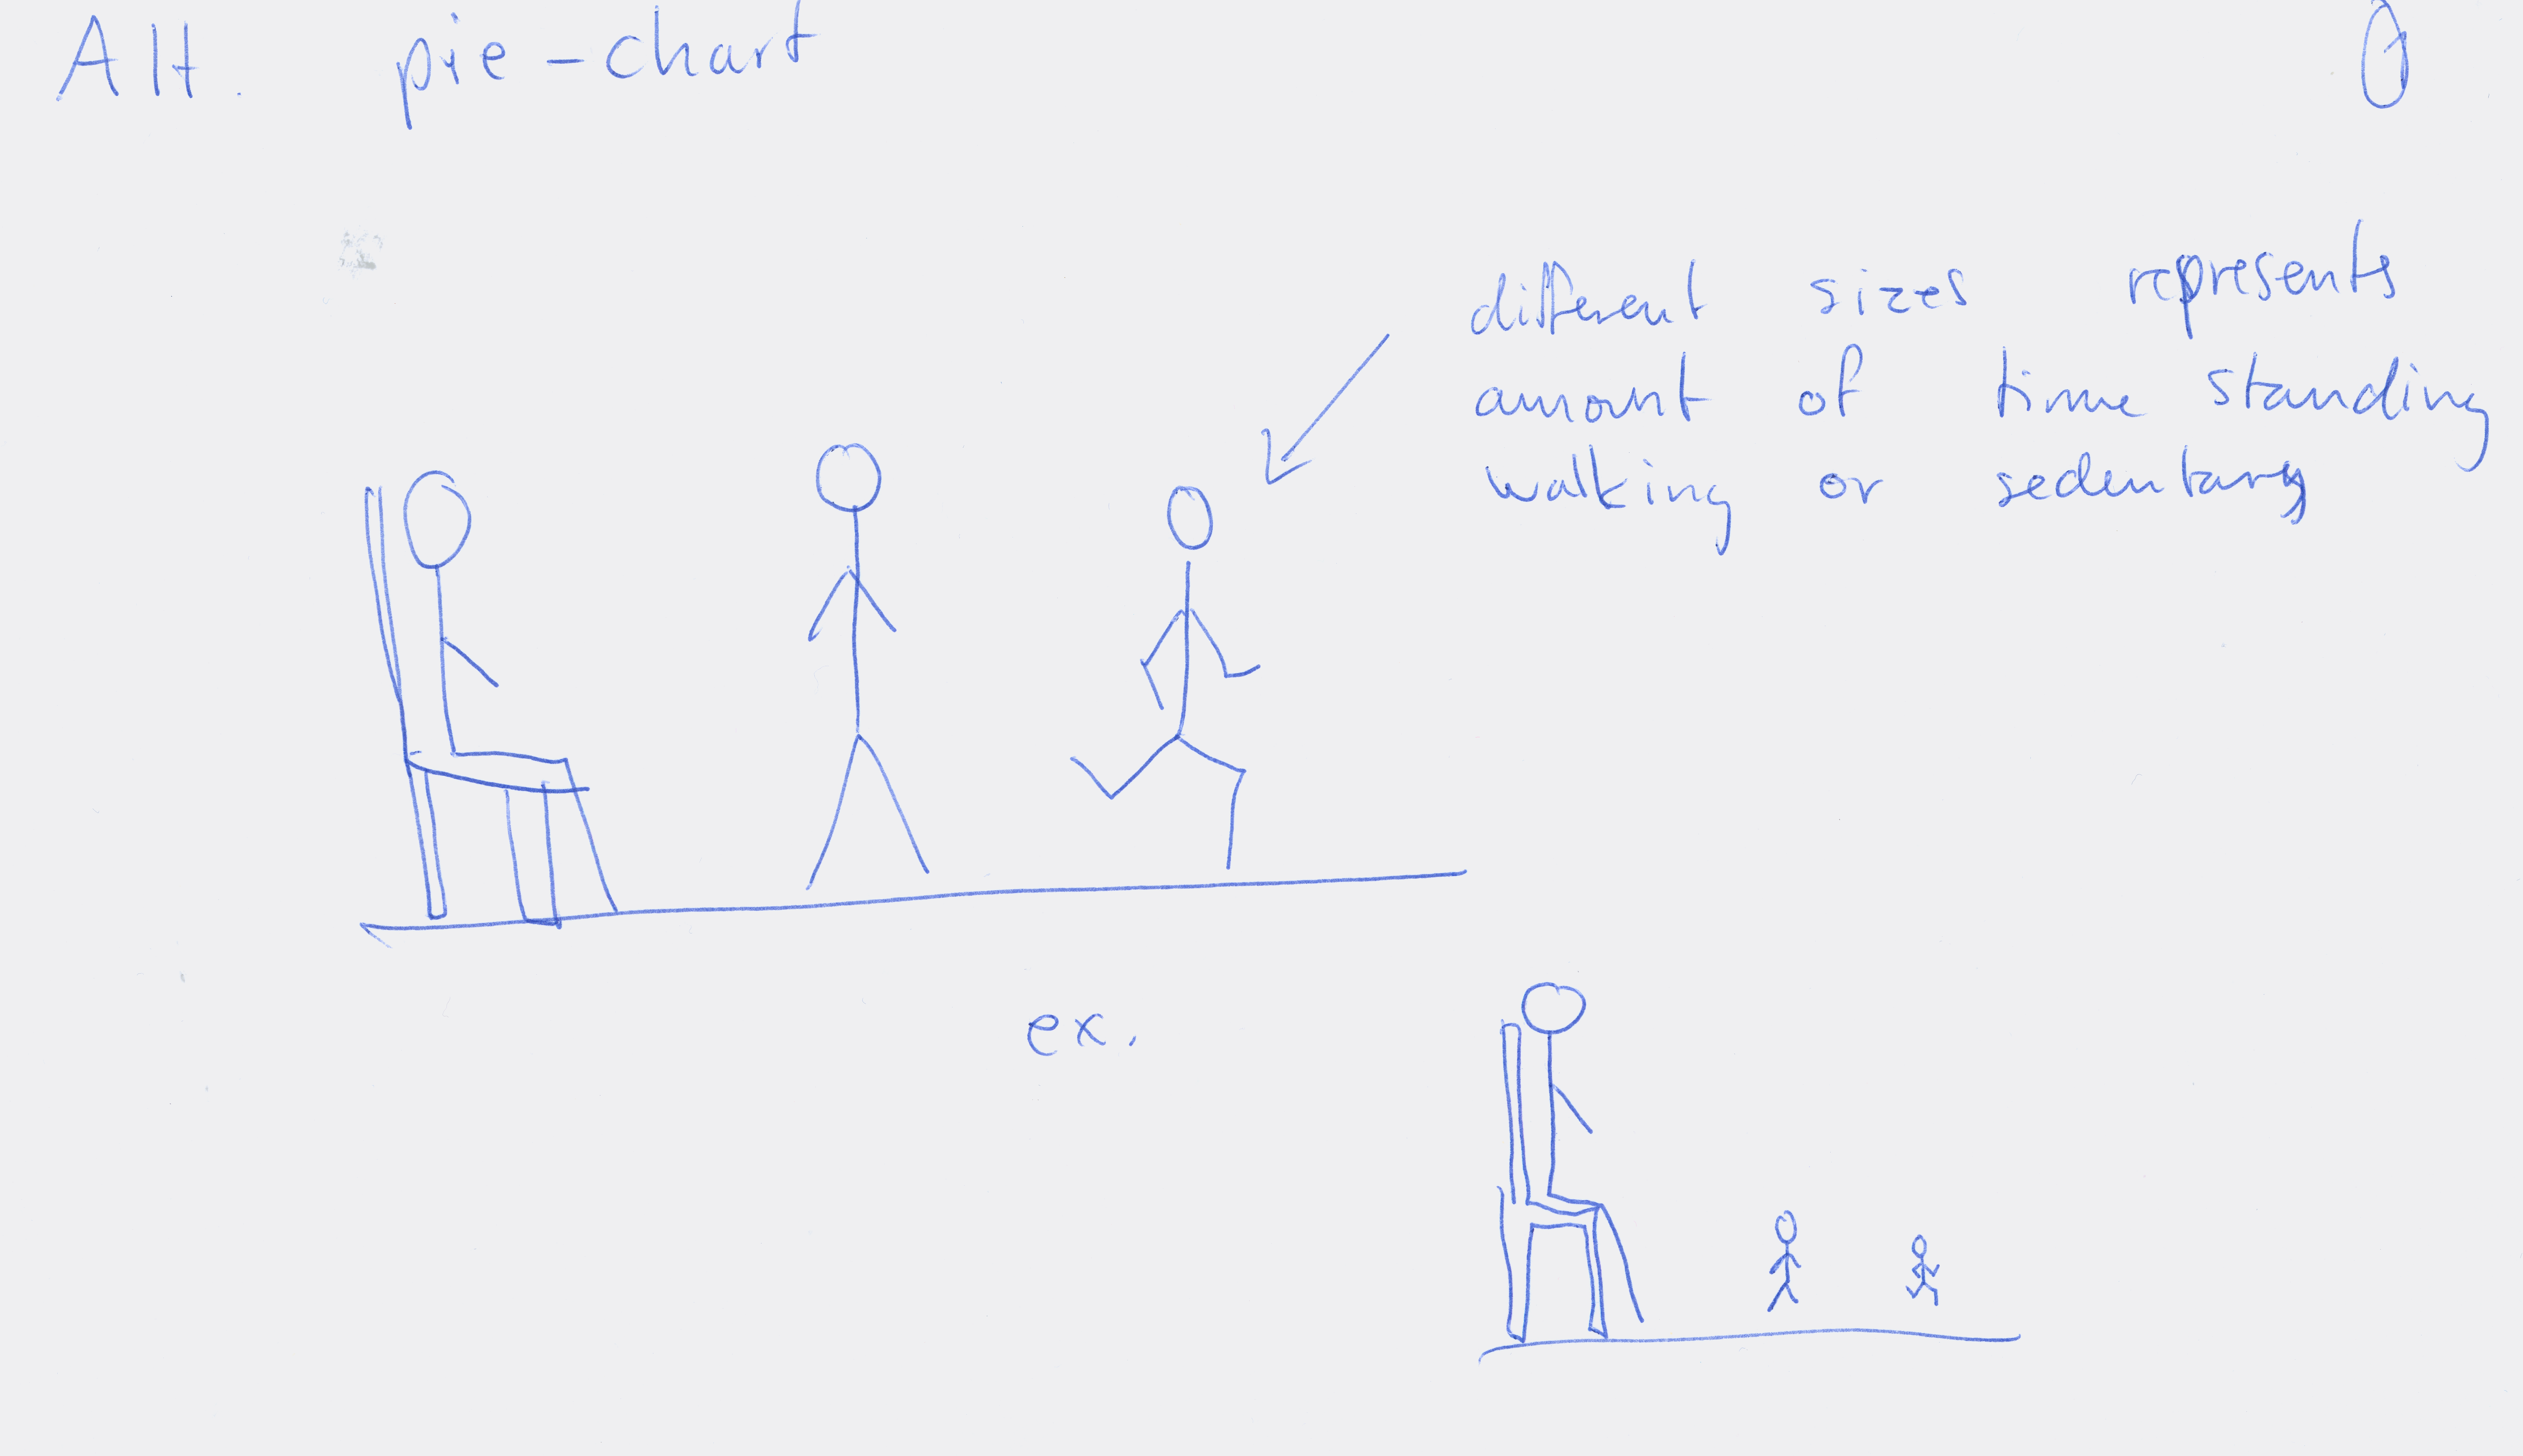
\includegraphics[width=0.7\textwidth]{stickSketch.png}
		\caption{\footnotesize Our first idea for a symbolic "pie chart"}
		\label{fig:symbolicPie}
\end{figure}

\subsubsection{Ball chart}
An alternative is to include more detail into a pie chart style, by using balls instead of normal pie slices. The balls are colour coded so that each colour reflects an activity state, while the size of the ball represent the continuous amount of time spent in the corresponding state. Each ball represents an interval of one of the classifications, so that many balls of one colour both represents the amount of that behaviour and shows how long each period of that behaviour was. Figure~\ref{fig:ballChart} shows an example of such a graph. The benefit with this type of graph is that one can easily identify long periods of sedentary behaviour. Taking small breaks with movement can help ``split up'' those balls, which is beneficial for ones health. By adding interactivity to the chart the user can select each ball and see what time it corresponds to. Overall the chart allows for the large balls to be easily spotted and the time of day quickly identified.

\begin{figure}[h!]
	\centering
		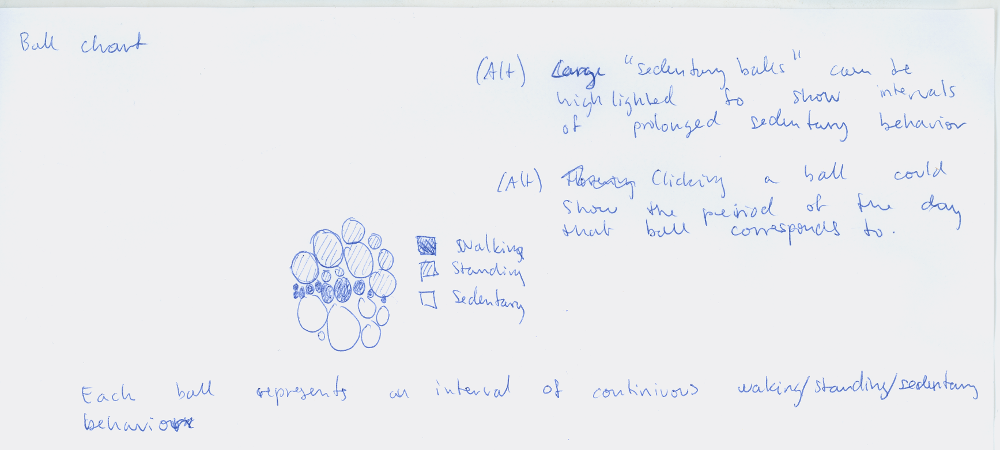
\includegraphics[width=0.7\textwidth]{ballChart.png}
		\caption{\footnotesize Rough drafts of the Ball chart}
		\label{fig:ballChart}
\end{figure}

\subsection{Timeline}
Timeline visualisations are effective at illustrating when various activities occurred during the day. The illustration uses a long horizontal bar that has different colours for different behavioural classification. These visualizations primarily address requirement IR3, IR5, and IR6. Such a bar can be used to identify points during the day where the subject is in a sedentary position for too long. By looking at multiple days, the user can detect patterns in the day where he needs to be more active.

\subsubsection{Continuous}
One approach to this visualization type is to create a continuous timeline that contains every little detail of activity. The continuous timeline is useful for quickly identifying periods of the day with unsatisfactory behaviour, but the detail can also be distracting and make it harder to read the graph.

\subsubsection{Blocks}
Instead of having a continuous scale, a blocked approach can be used, as seen in figure \ref{fig:timelineBlocks}. The timeline would be divided into 24 blocks, each block corresponding to an hour of the day. A gradient colour scale is used to represent the amount of activity inside the hour block. This makes it easy to identify hours of the day where the patient is inactive. 

\begin{figure}[h!]
	\centering
		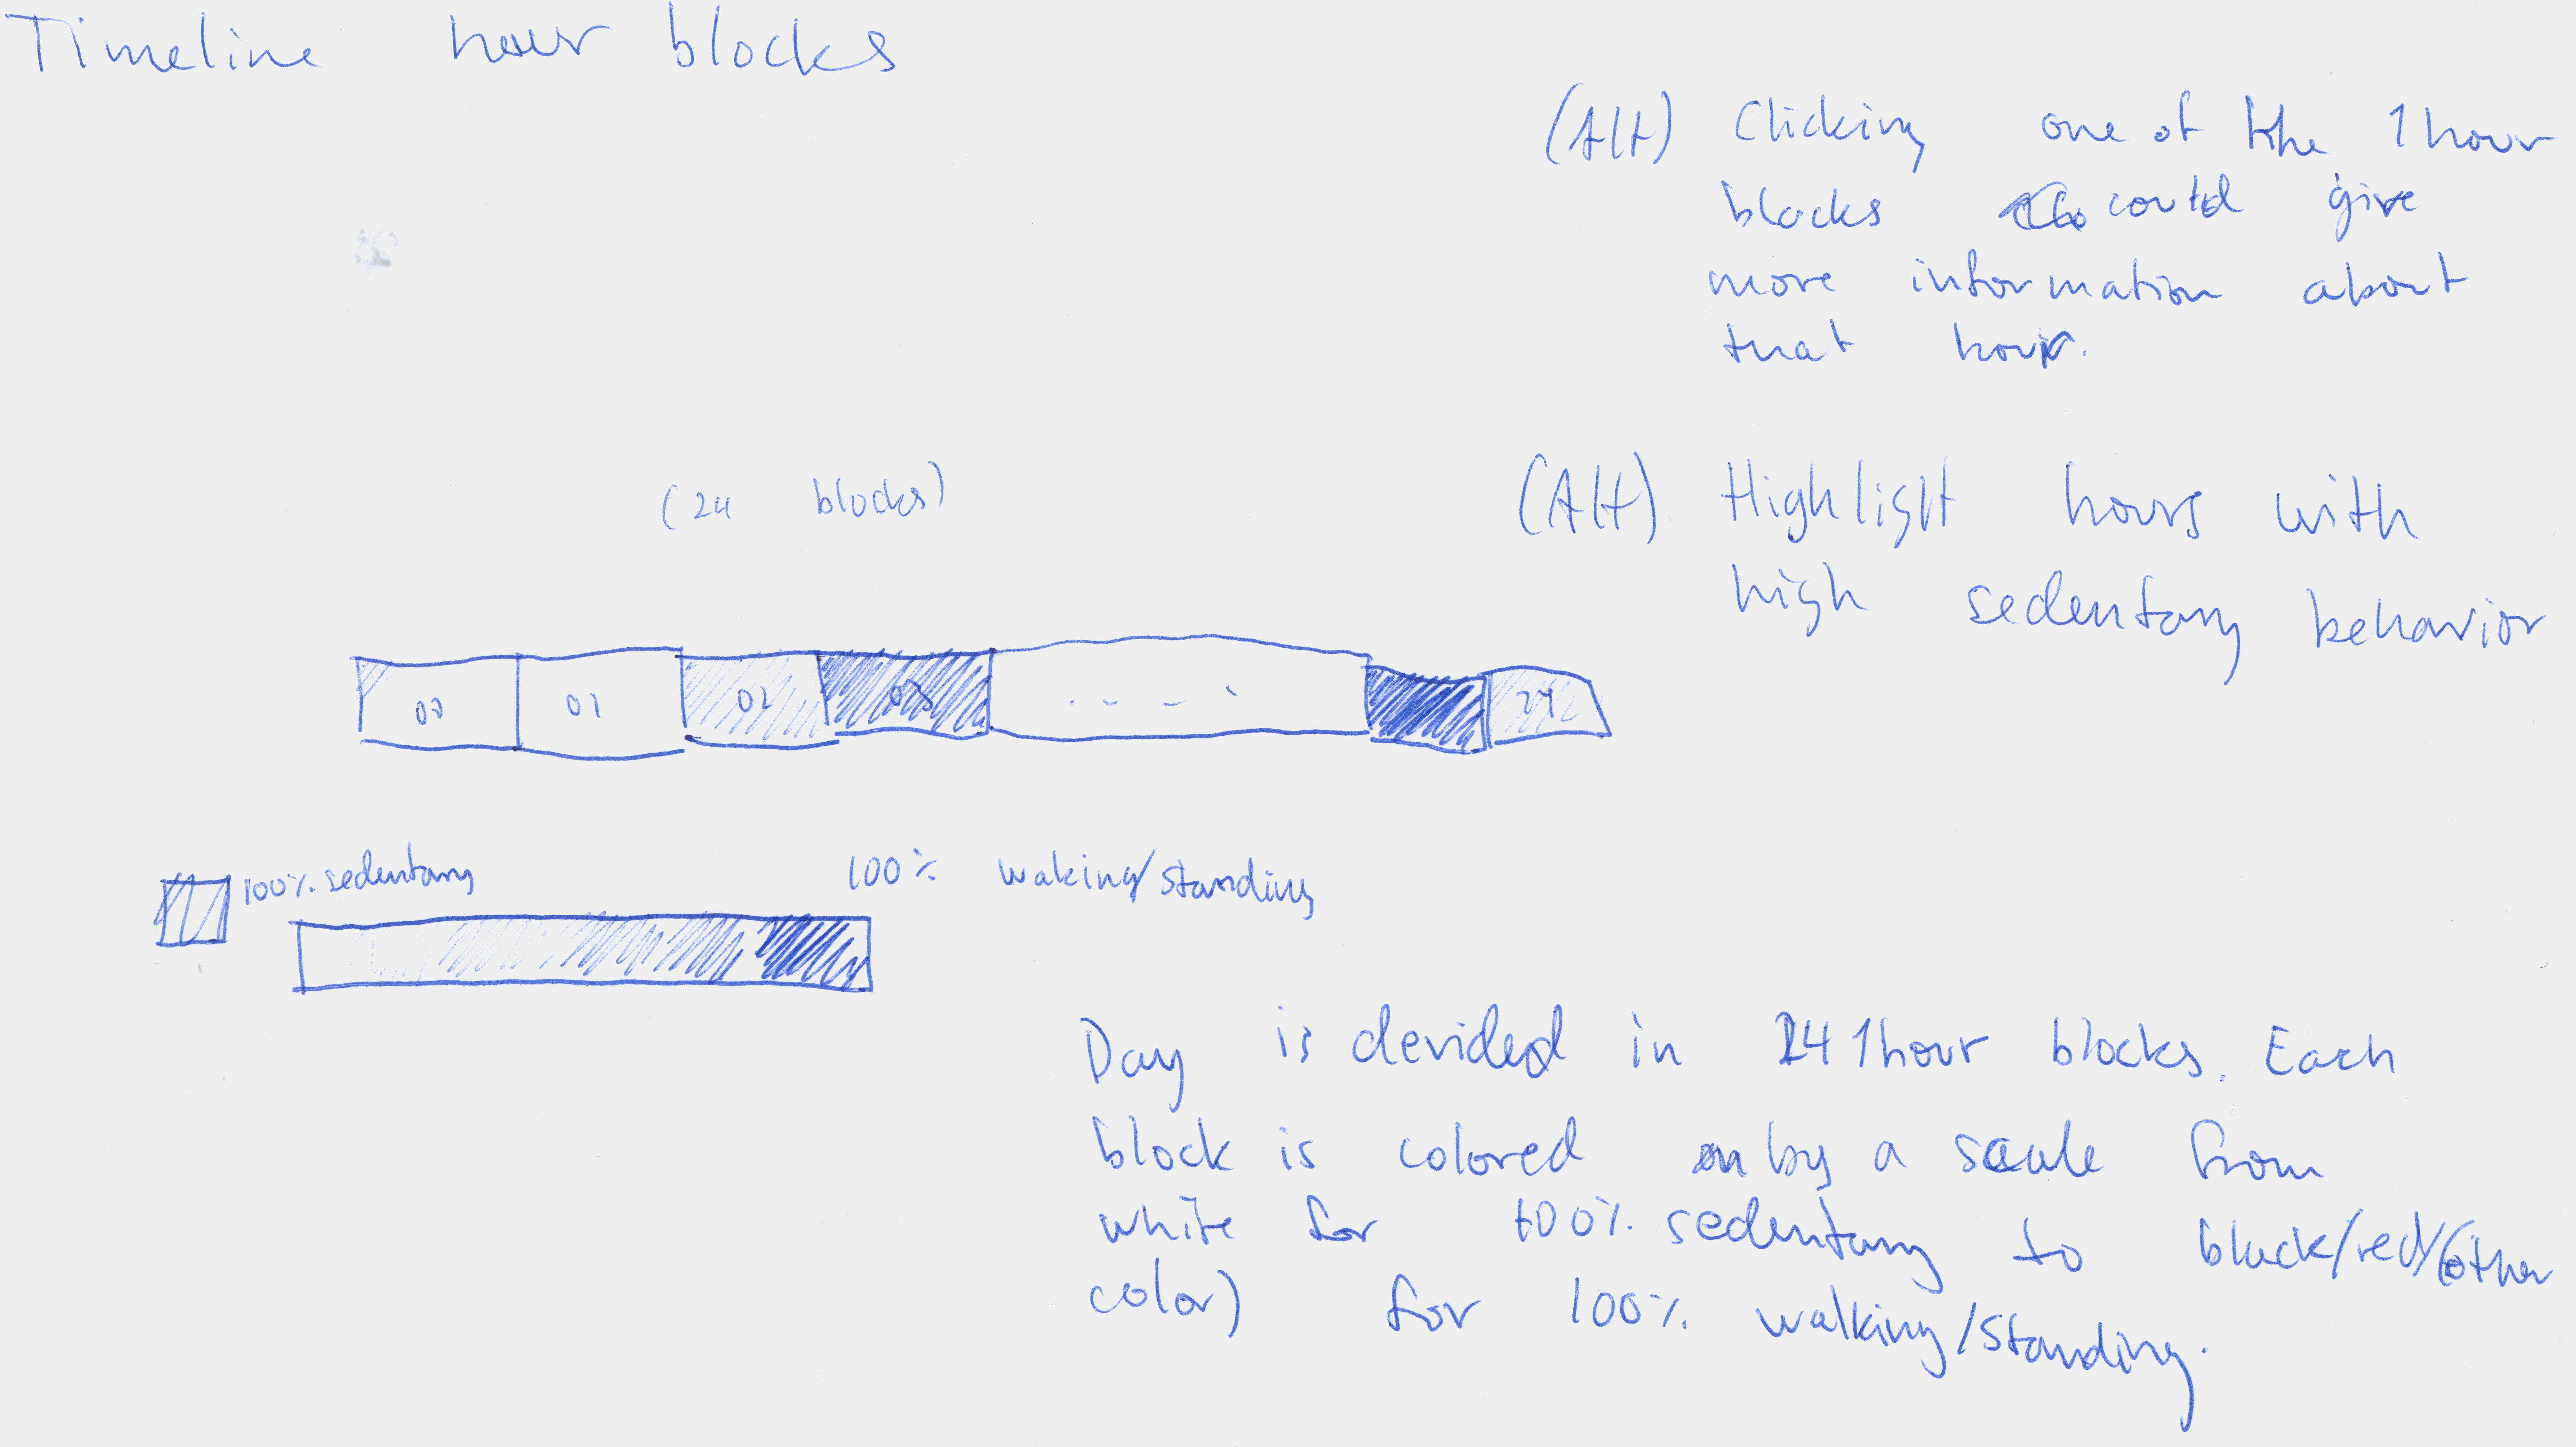
\includegraphics[width=0.7\textwidth]{timelineBlocksSketch.png}
		\caption{\footnotesize Timeline with hour blocks}
		\label{fig:timelineBlocks}
\end{figure}

\subsubsection{Clock}
A timeline may need some explanation before the user understands it properly. By creating two clocks instead of a long horizontal bar the user can more intuitively understand what the visualization is presenting. Since a clock has only 12 hours, two clocks are created to represent the entire day. To make it easier to identify day and night, a descriptive background is necessary, see figure \ref{fig:clock12}.

\begin{figure}[h!]
	\centering
		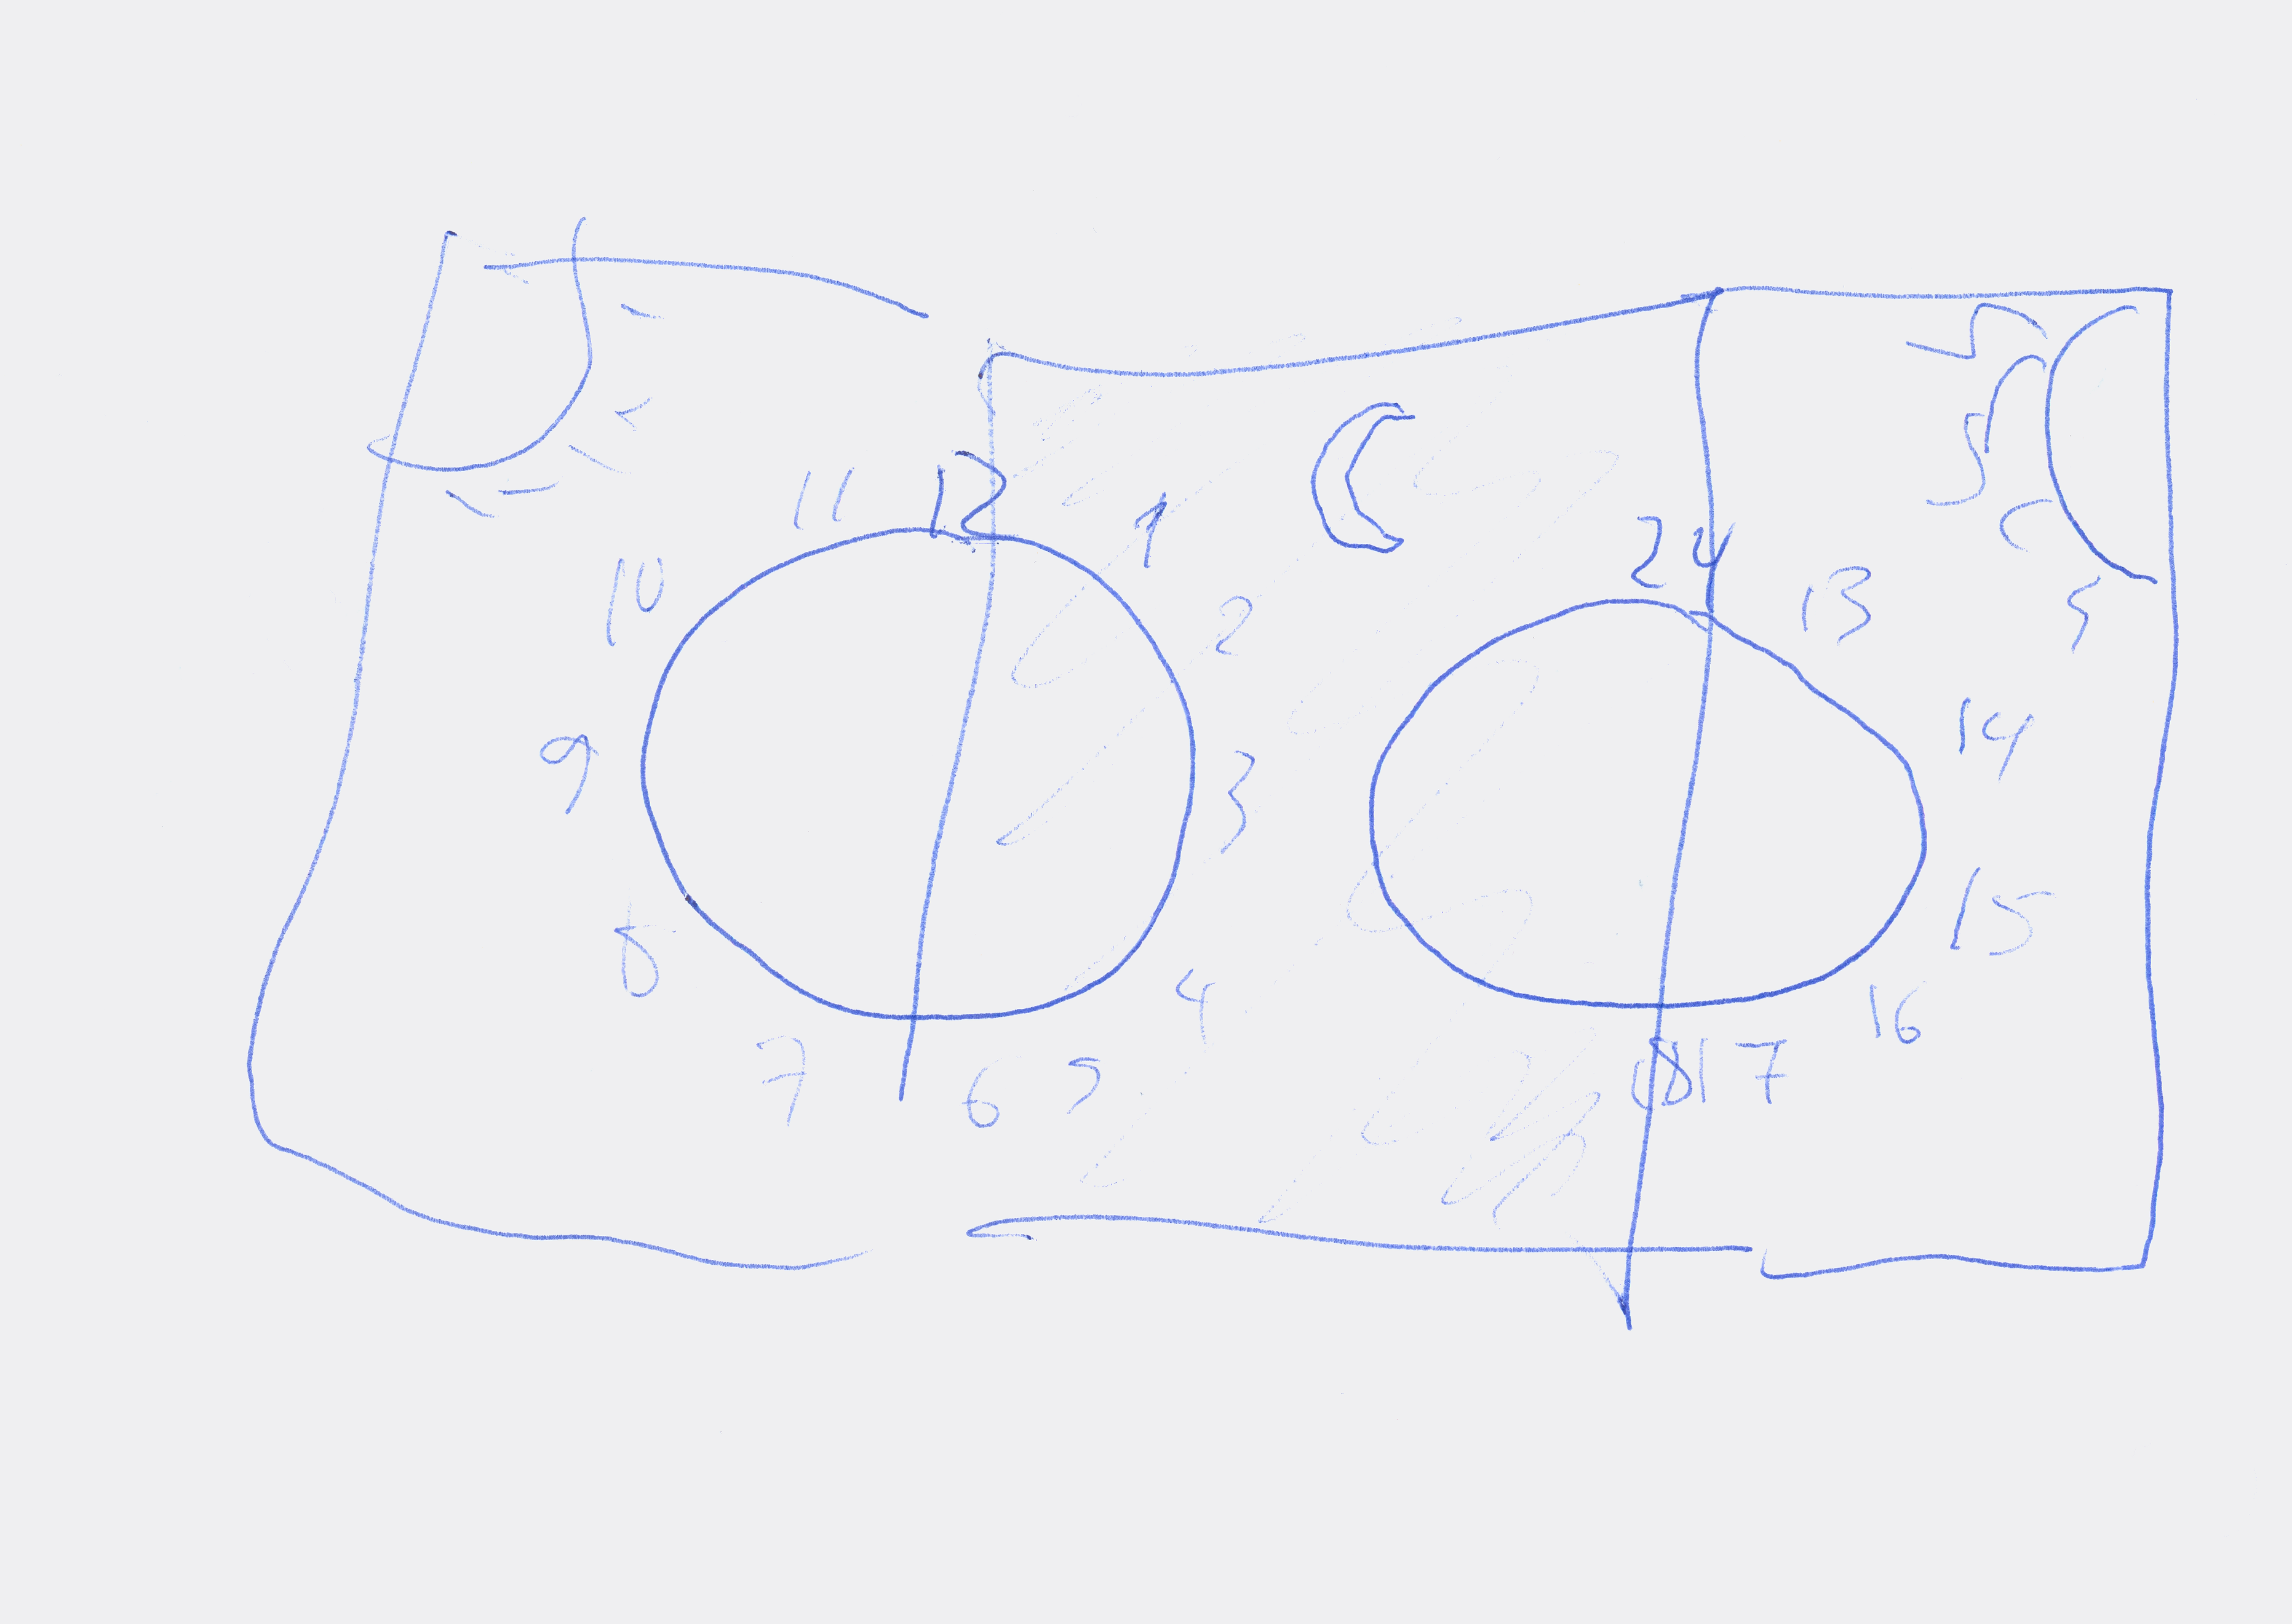
\includegraphics[width=0.7\textwidth]{clock12Sketch.png}
		\caption{\footnotesize Two 12 hour clocks show the activity of the day.}
		\label{fig:clock12}
\end{figure}

Another approach is to use one 24 hour clock. This makes it easier to see the transition between AM and PM, but 24 hour clocks are not natural, so it might be problematic for the user to understand.

\subsection{Week overview}
Getting an overview of the week as a whole can be useful as an introduction. By looking at an overview the user can quickly identify bad days that can then be investigated further. In other words they cover requirement IR1 and IR4. These visualizations could also be used as the top level of an interactive application. Each day could then be clicked to show either a timeline or pie chart.

\subsubsection{Day classification}
By calculating the overall activity level and classifying the days into three categories the user can easily see which days he need to be more active and which days the activity level is satisfactory. In our sketch, see figure \ref{fig:smileyWeek} the three different classifications are illustrated by smilies (smiling face for active days, and sad face for inactive days).

\begin{figure}[h!]
	\centering
		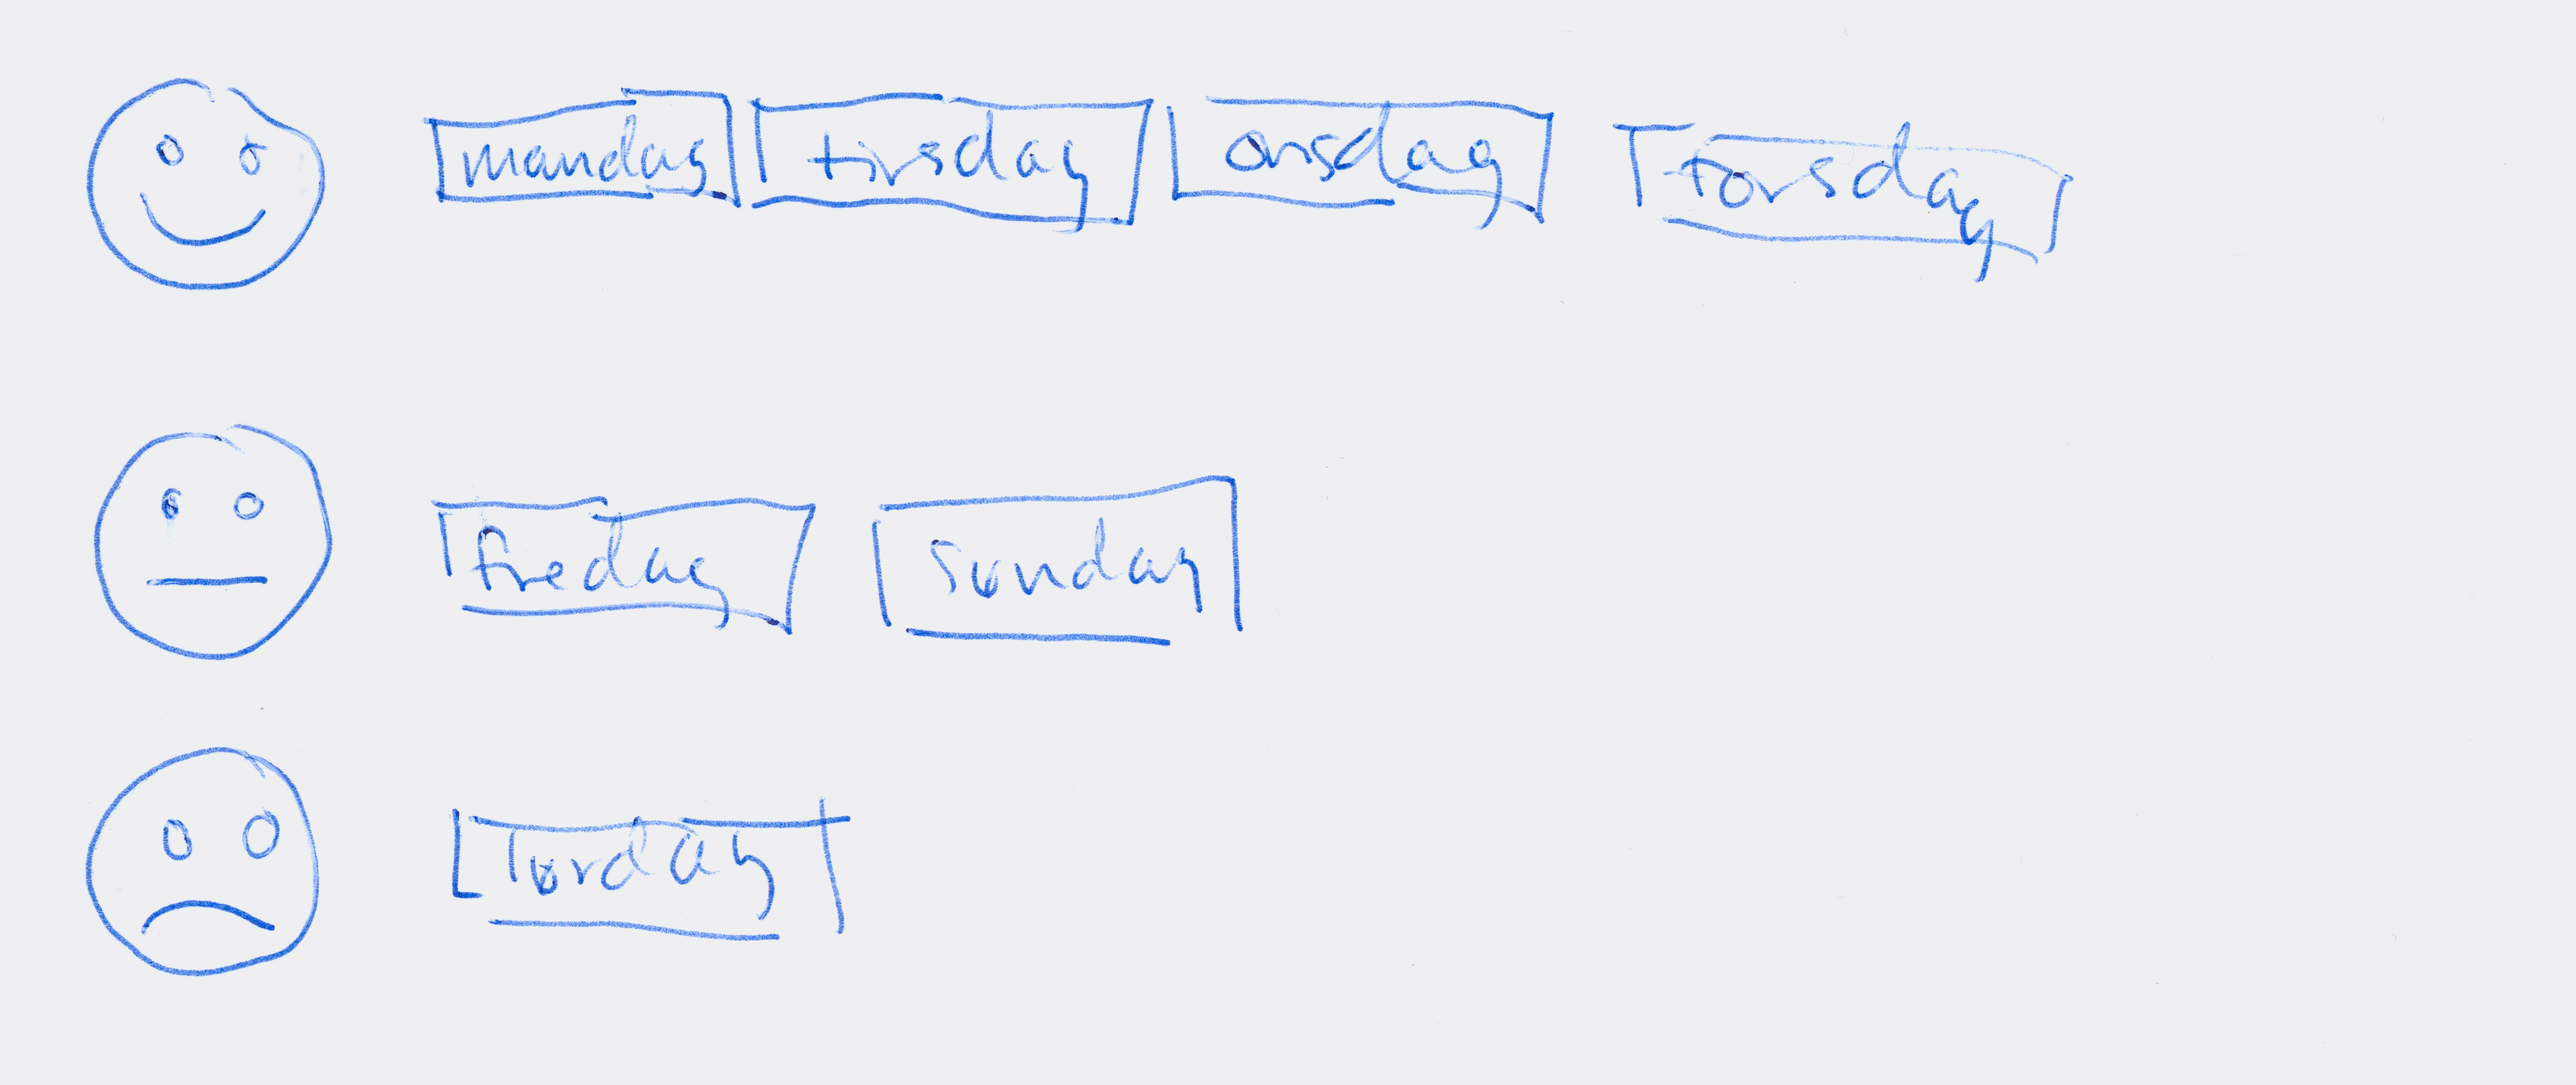
\includegraphics[width=0.7\textwidth]{smileyWeekSketch.png}
		\caption{\footnotesize Week overview with each day classified into one of three categories.}
		\label{fig:smileyWeek}
\end{figure}

A more complex version of the above chart, see figure \ref{fig:detailedWeek} is to show a square for each day, while still using the same classification into sad and happy smilies. Each day square will then contain 24 smaller squares that represent each hour of the day. The small hour square are coloured with a gradient to show the activity level for that hour. With this chart you can get an overview of the week as a whole, and identify what hours of the inactive days had the most sedentary behaviour. 

\begin{figure}[h!]
	\centering
		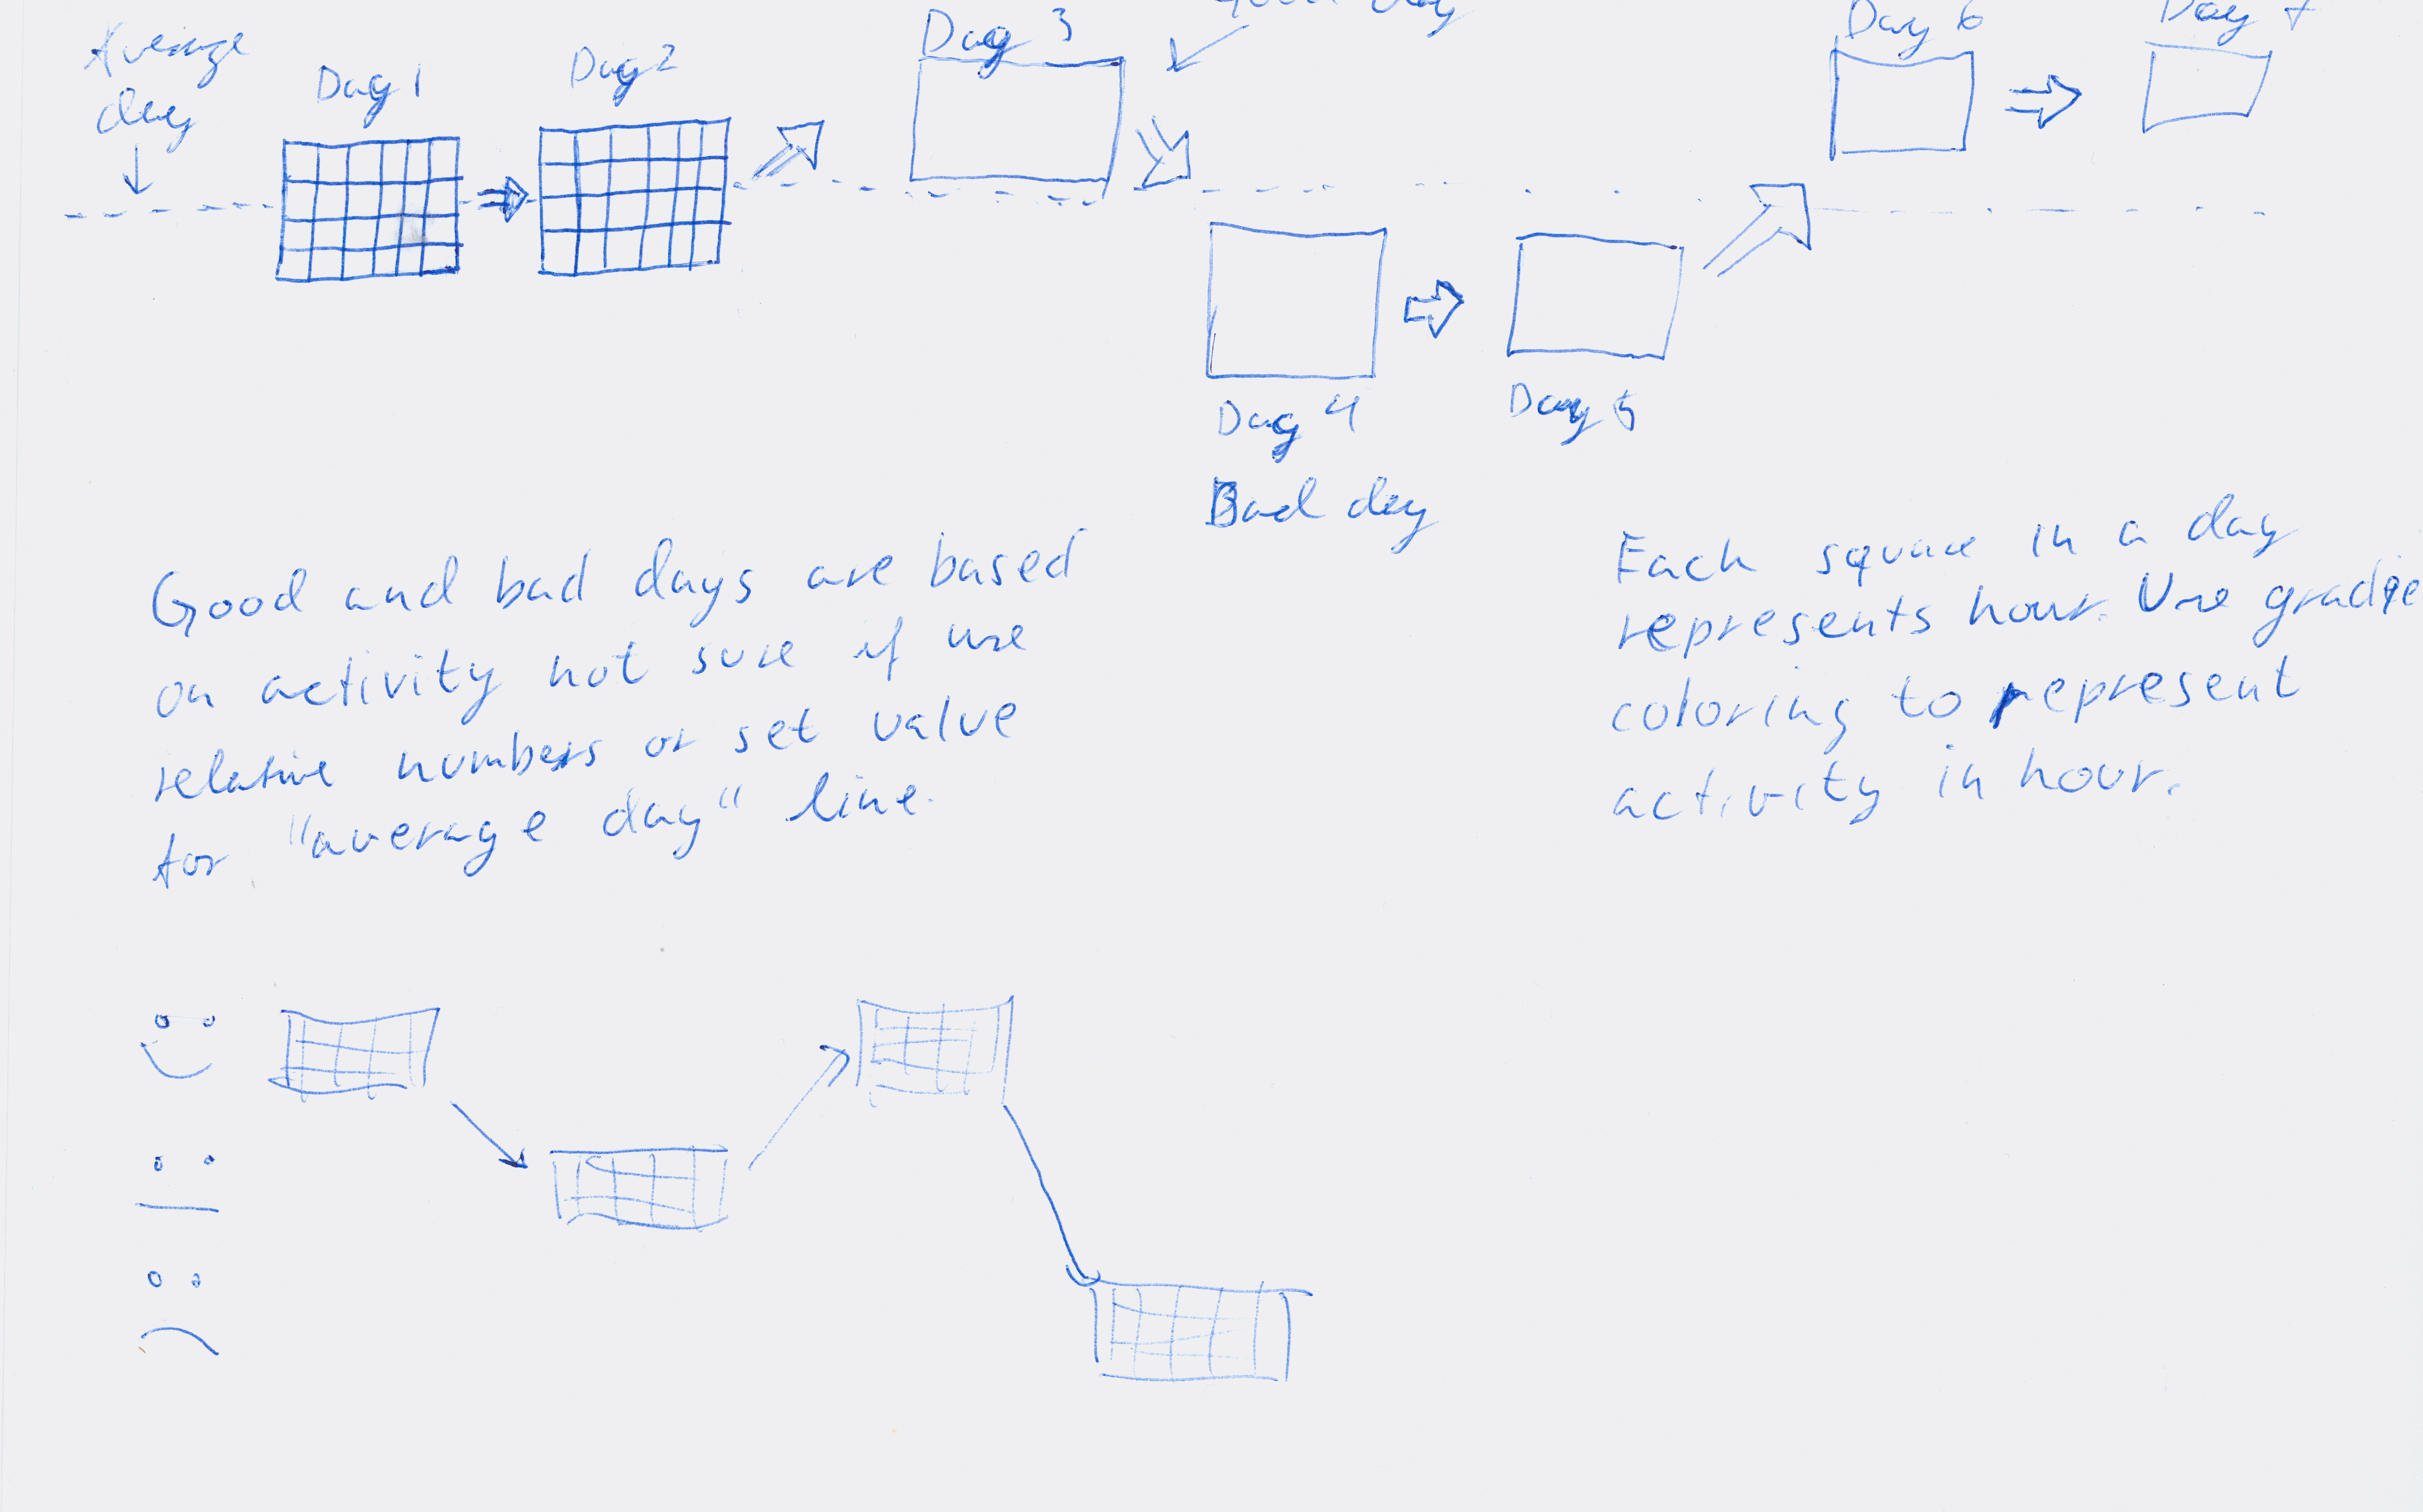
\includegraphics[width=0.6\textwidth]{detailedWeekSketch.png}
		\caption{\footnotesize Some explanation here.}
		\label{fig:detailedWeek}
\end{figure}

\section{Programming framework}
The task was to create custom visualizations form data gathered the activPAL sensor. The choice of programming tools fell on HTML5 and an open source JavaScript framework called D3.js.

\subsection{HTML5}
HTML is a markup language for the creation of web pages. HTML describes the structure and the contents of the web page. In later years, the need for advanced styling and complex interaction with web pages has made CSS and JavaScript increasingly popular. HTML5 was created as a response to this, HTML5 is an umbrella term for creating web pages using HTML5, CSS3 and JavaScript.

HTML5 has simplified the syntax compared to earlier versions. New tags have been added to better represent the modern web page elements. Other features include media tags which greatly simplifies adding multimedia content, such as playing audio and video files. More importantly for our project is the extensive support for interactive and animated graphics through the \emph{canvas-} and \emph{svg}-tag.

The new features of HTML5 and CSS3 make it much easier to create web applications for multiple platforms and screen sizes. After the smartphone and tablet revolution, creating responsive and adaptable websites has become more important. The new features included in HTML5 give large amount of flexibility with respect to the user interface and graphical visualizations.

\emph{Cascading Style Sheets} (CSS) is a language used to describe the styling of an HTML document. CSS documents describes the size, color and look of HTML elements. A new feature in CSS3, which is part of HTML5, is \emph{Media Queries}. With Media Queries it is possible to specify different styling relative to the size of the screen. This functionality is useful when creating applications that target devices with different screen sizes, such as smartphones, tablets and laptops. 

\subsection{Data-Driven Documents}
JavaScript is the main scripting language for web pages. It is a client-side scripting language that allows programmers to add functionality to otherwise static HTML-pages. While CSS3 takes care of the styling of HTML-elements, JavaScript is used to create customized behaviour. All modern browsers have JavaScript engines/interpreters that compile and run JavaScript code.

JavaScript is now an industry standard maintained by ECMA International. The standardized version of the script is named ECMAScript. Today, the names ECMAScript and JavaScript are used interchangeably, and JavaScript is often used to refer to ECMAScript. Because different browsers have different implementations of the JavaScript engine, slight variations in the way JavaScript code will run on these browsers exists.

Together with HTML5 and CSS3, JavaScript is great for creating web applications that can be designed to run on both mobile and stationary devices. JavaScript has a multitude of useful open source libraries that can be used to create complex user interaction, animation, and custom graphics.

One of the challenges in this project was to create different visualizations to represent the activity patterns of subject. Creating custom graphics in HTML5 can be done using both the canvas- and the svg-tag. In this project \gls{svg} is used. \gls{svg} is an image format that uses XML encoding to define shapes, lines, colors, and text. One benefit of this, compared to other image formats, is that details in \gls{svg}-images will not be lost when zooming. All popular browsers, and most mobile devices, support rendering of the \gls{svg}-images.

Creating graphics using svg-tags directly is cumbersome and time consuming. \gls{d3} is an open source framework that greatly simplifies this task. \gls{d3} is written in JavaScript and designed to be used in combination with HTML5. The framework can be used both to create new \gls{svg} images from scratch or modify and edit existing images. Another feature is the ability to easily add interactivity and animation to the \gls{svg}-elements. HTML5 in combination with \gls{d3} gives us flexibility to create almost any type of visualization and adding interactivity and animation to it.

%Her skriver du bare om hvordan ting ser ut, burde vi relatere det mer til sketchene, eller user requireents som jeg nevnte i paper sketches, slik at det blir en mer ``rød tråd'' over det hele. Det er kanskje ikke nødvendig her, men det burde i såfall gjøres under prototype 2. Ellers liker jeg oppstett på kapitellet, jeg har gått gjennom og endret litt tekst her og der samt gramatiske feil
\section{Running prototype}
9 of the paper prototypes were selected for implementation for the system shown to focus group 1. The diagrams were given ID, as seen in the table~\ref{tab:runProtDesc1}. Figure~\ref{fig:runProt1} shows a screen shot of the different types of diagrams. 

\begin{table}[h!]
  \begin{center}
  \begin{tabular}{|c|p{10cm}|}
    \hline
    \textbf{ID} & \textbf{Description} \\ \hline
    U1 & Classifies each day of the week into either of three categories: High, medium and low activity. \\ \hline
    U2 & Classifies each day of the week as in U1. Also shows 24 squares for each day, each square representing one hour. The activity level for each hour is displayed using a gradient. \\ \hline
    F1 & Pie chart showing the amount of activity for each day. \\ \hline
    F2 & Same as F1, but with boxes instead of pie slices and descriptive figures inside each box. \\ \hline
    F3 & Bubble chart. Divides the pie slices of F1 into bubbles each bubble representing one interval of activity (ex. 2 hours of non-stop sedentary behaviour). \\ \hline
    T1 & Timeline of 24 squares, each square represents 1 hour of activity. The amount of activity in that hour is displayed using a gradient. \\ \hline
    T2 & Rectangle shaped timeline, showing the type using colour coding. \\ \hline
    T3 & Two 12-hour clocks showing the activity type using colour coding. \\ \hline
    T4 & One 24-hour clock showing the activity type using colour coding. \\ \hline
  \end{tabular}
  \end{center}
  \caption{Diagrams implemented for the first focus group.}
  \label{tab:runProtDesc1}
\end{table}

The two diagrams U1 and U2 are week overviews. These are designed to give you a quick overview of the week. U2 experiments with adding more detail, and contains 24 small squares for each day that represent the activity of each hour. Holding the mouse cursor over a day in U1 will show the percentage of each type of activity for that day. Holding the mouse cursor over a square in U2 will show the percentage of each type of activity for the hour that square represents.

\begin{figure}[h!]
  \centering
  \begin{subfigure}[b]{0.45\textwidth}
    \centering
    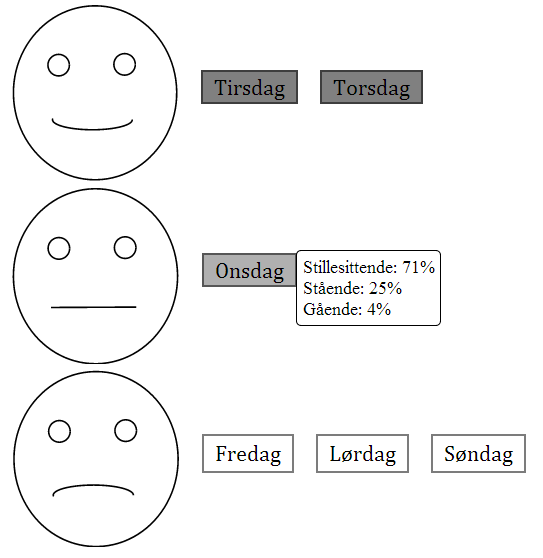
\includegraphics[width=\textwidth]{u1First.png}
    \caption{U1}
  \end{subfigure}
  \begin{subfigure}[b]{0.45\textwidth}
    \centering
    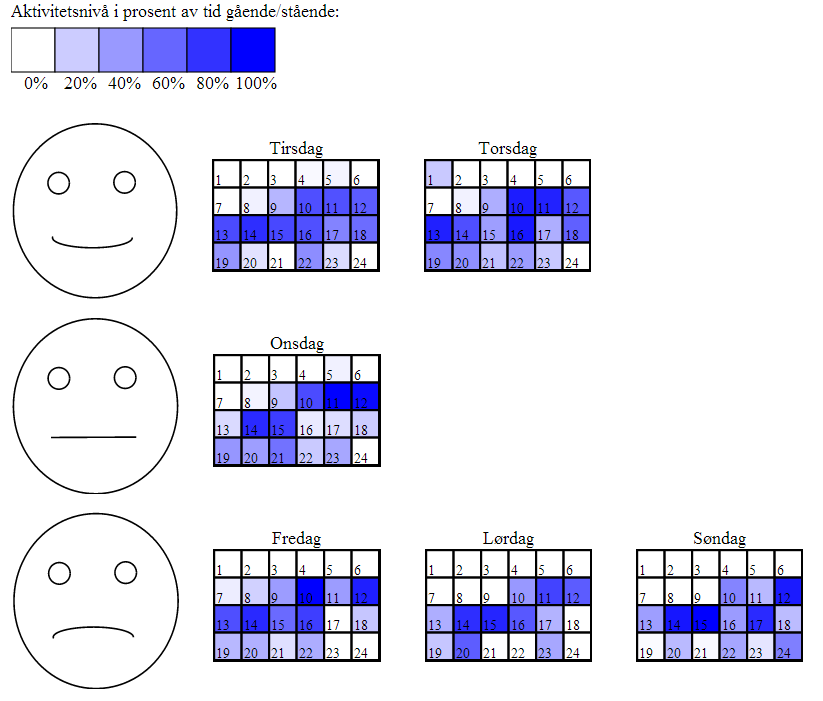
\includegraphics[width=\textwidth]{u2First.png}
    \caption{U2}
  \end{subfigure}
  \caption{Week overview charts.}
  \label{fig:runProt1}
\end{figure}

%Review: Tror du har mistet now tekst det står bare ``When showing the entire week'' og så slutter det.
Diagrams F1, F2 and F3 are the fractional charts*. These diagrams shows the fraction of each type of activity for a day. F1 and F2 are similar, F1 is a standard pie diagram while F2 uses boxes with figures describing the activity. F1 and F2 has two types of view modes: one day or the entire week. When showing the entire week. F3 is more complex, this diagram shows each interval of activity as a ball. Long intervals of activity is represented by a larger ball than small intervals of activity. This graph can therefore be used both to see the distribution of the different activity types and, more importantly, the length of continuous activity, or sedentary behaviour. This is useful when you want to identify if the patient has very long periods of sedentary behaviour, or if the patient walks continuously for a long time, or takes small brakes. Holding the mouse cursor over a bubble shows you the time the activity interval occurred as well as the length of the interval. F3 also offers a highlighting mode, when active intervals of more than 1 hour are highlighted.

\begin{figure}[h!]
  \centering
  \begin{subfigure}[b]{0.45\textwidth}
    \centering
    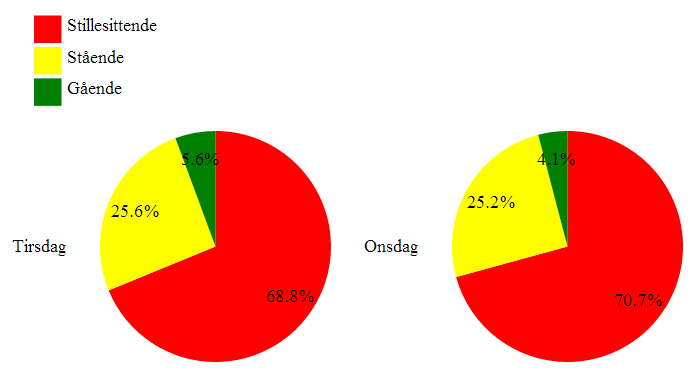
\includegraphics[width=\textwidth]{f1First.png}
    \caption{F1}
  \end{subfigure}
  \begin{subfigure}[b]{0.45\textwidth}
    \centering
    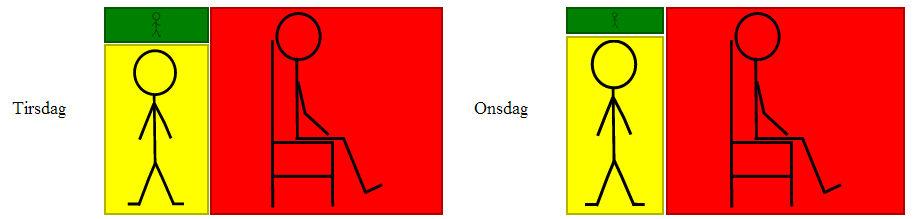
\includegraphics[width=\textwidth]{f2First.png}
    \caption{F2}
  \end{subfigure}
  \\
  \begin{subfigure}[b]{0.45\textwidth}
    \centering
    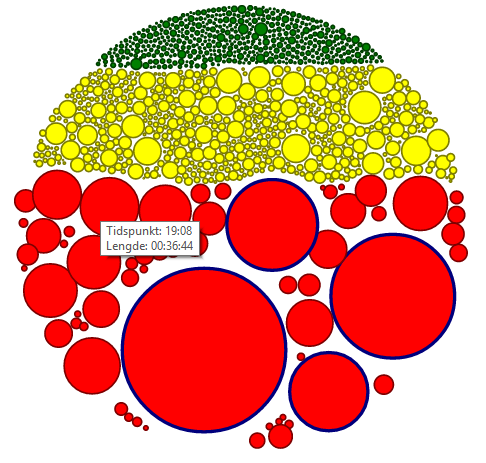
\includegraphics[width=\textwidth]{f3First.png}
    \caption{F3}
  \end{subfigure}
  \caption{Fractional charts*}
\end{figure}

T1, T2, T3 and T4 are diagrams that show timelines or clocks. These diagrams are useful to see when the patient was active during the day. T1 shows 24 squares each representing an hour of the day. The percentage of activity (walking and standing) is shown as a gradient in each square. Holding the cursor over a square gives you the percentage of each type of activity. T2 is also a timeline, but here the data is not aggregated so the timeline is continuous and shows the activity at a much more detailed level. This is useful if you need to see when in a particular hour activity was performed. It also distinguishes between standing and walking activity. T3 and T4 are also show the activity continuously but they use a clock instead of a timeline to illustrate when on they day the activity occurred. T3 uses two 12 hour clocks, while T4 uses a single 24-hour clock. Diagrams T2, T3 and T4 can toggle highlighting. When highlighting is toggled sedentary behaviour longer than 1 hour is highlighted with blue. All T-diagrams can be viewed one day at a time or the entire week all at once. 

\begin{figure}[!h]
  \centering
  \begin{subfigure}[b]{0.45\textwidth}
    \centering
    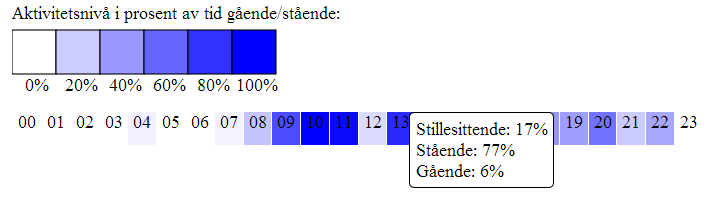
\includegraphics[width=\textwidth]{t1FirstSingle.png}
    \caption{T1 day.}
  \end{subfigure}
  \begin{subfigure}[b]{0.45\textwidth}
    \centering
    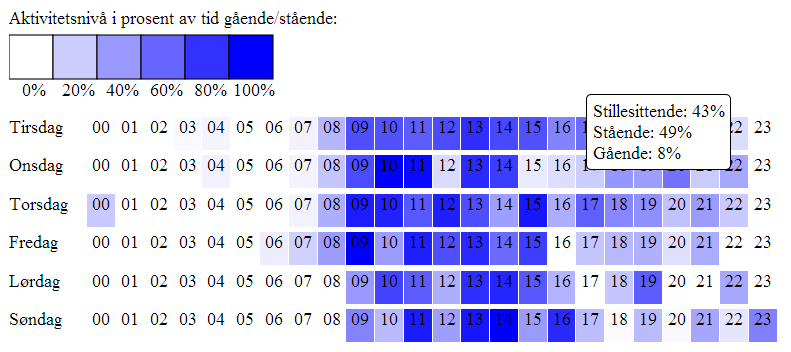
\includegraphics[width=\textwidth]{t1FirstWeek.png}
    \caption{T1 week.}
  \end{subfigure}
  \\
  \begin{subfigure}[b]{0.45\textwidth}
    \centering
    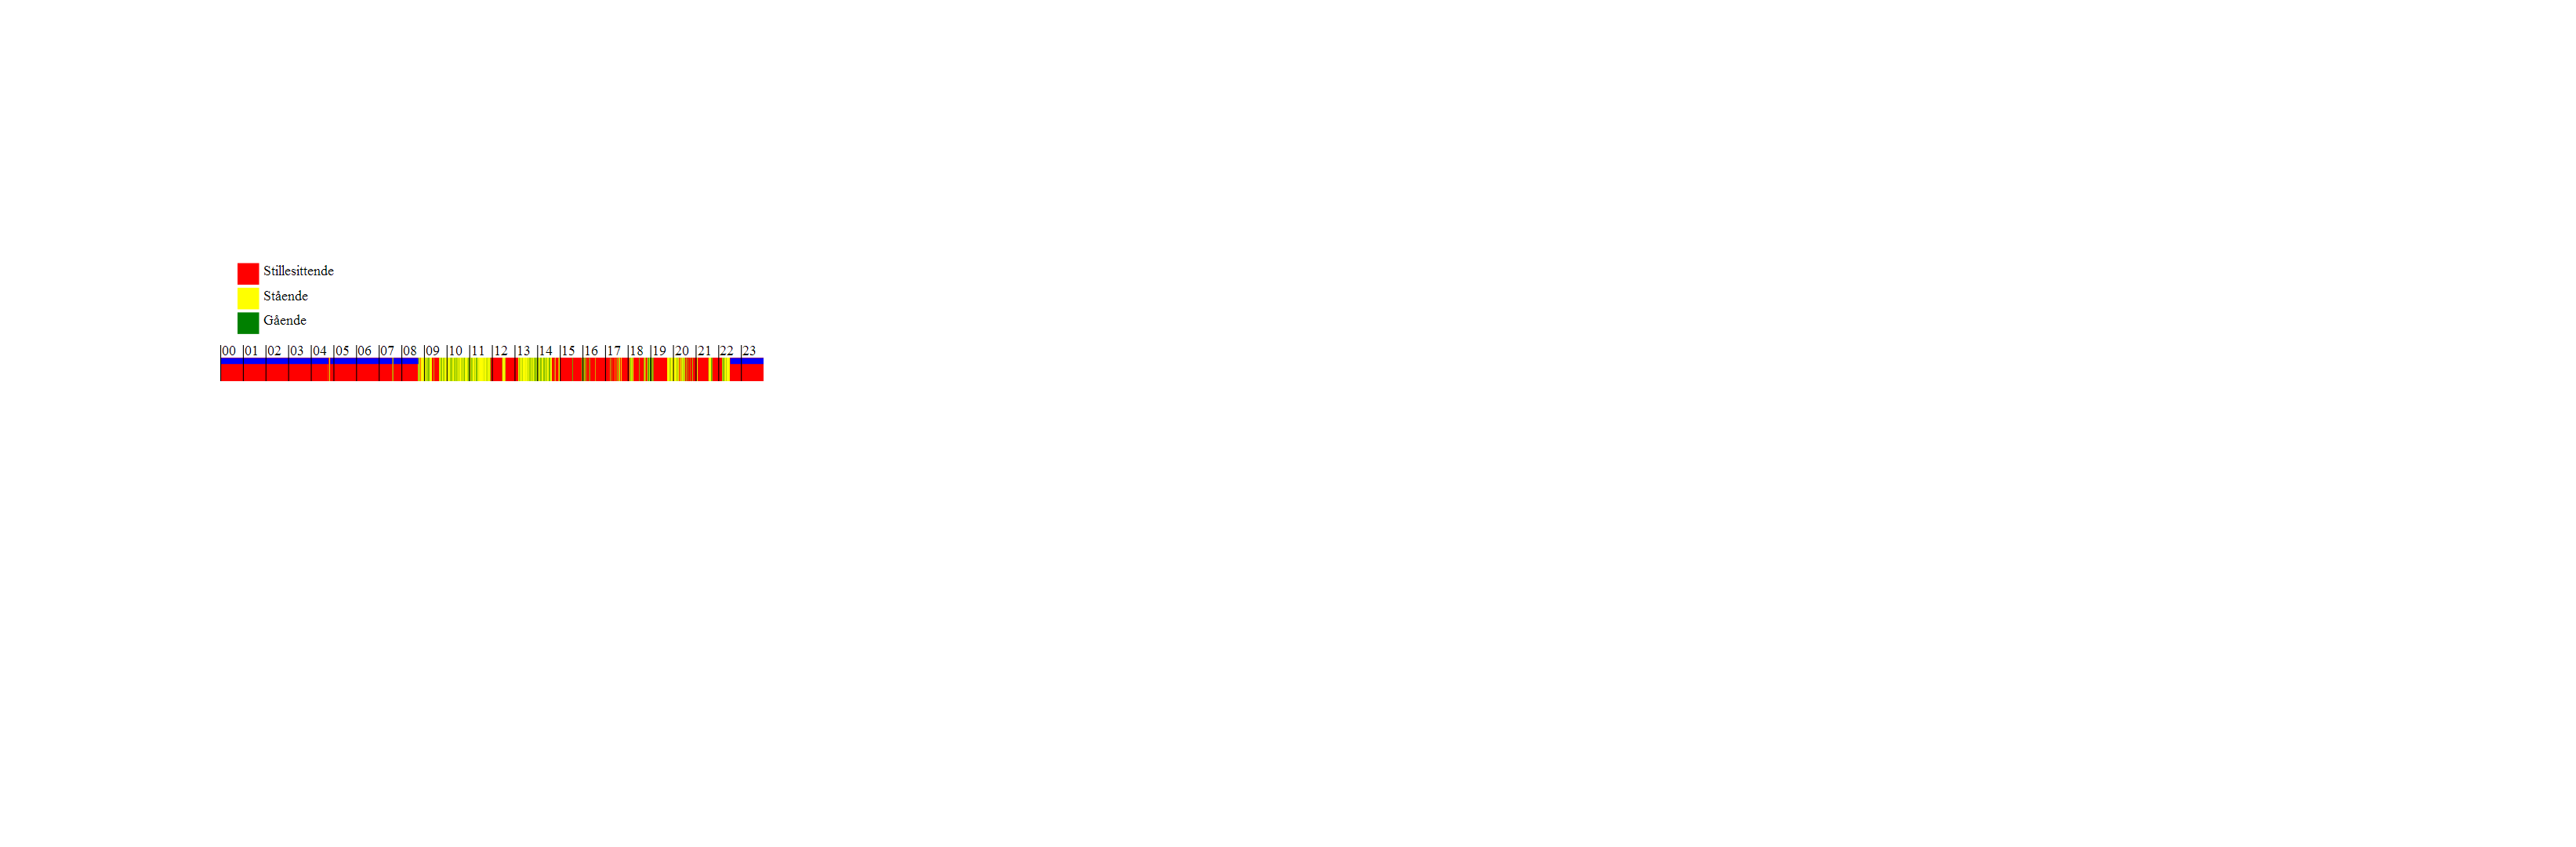
\includegraphics[width=\textwidth]{t2FirstSingle.png}
    \caption{T2 day.}
  \end{subfigure}
  \begin{subfigure}[b]{0.45\textwidth}
    \centering
    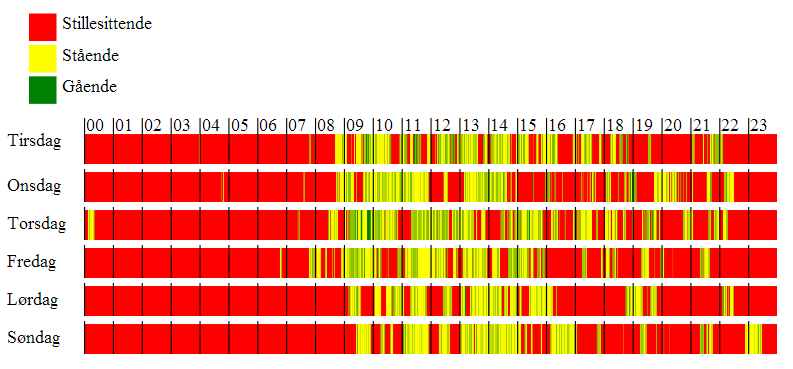
\includegraphics[width=\textwidth]{t2FirstWeek.png}
    \caption{T2 week.}
  \end{subfigure}
  \\
  \begin{subfigure}[b]{0.45\textwidth}
    \centering
    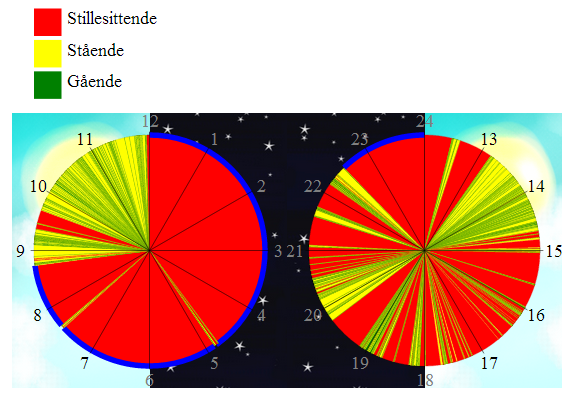
\includegraphics[width=\textwidth]{t3First.png}
    \caption{T3}
  \end{subfigure}
  \begin{subfigure}[b]{0.45\textwidth}
    \centering
    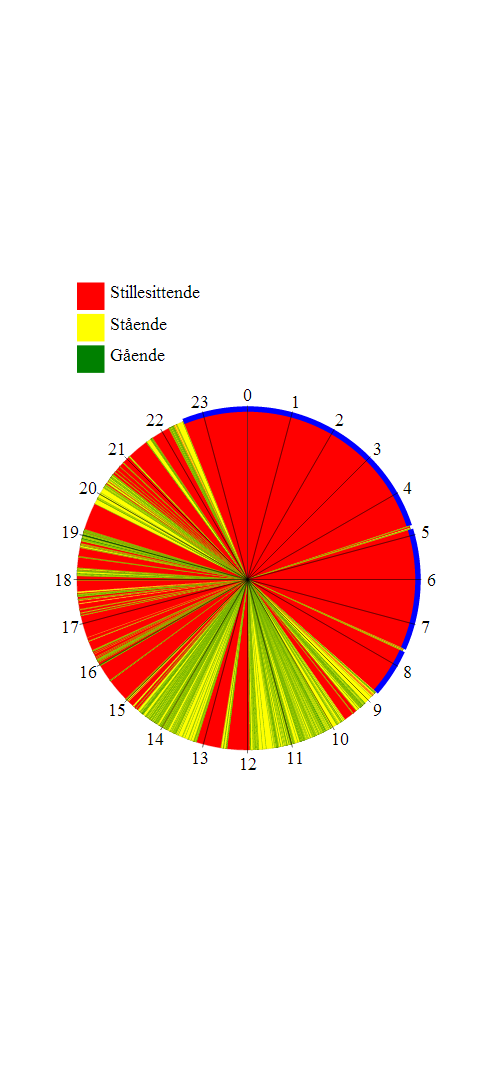
\includegraphics[width=\textwidth]{t4First.png}
    \caption{T4}
  \end{subfigure}
\end{figure}  

\chapter{Focus group 1}
%Remember to write about the duration

\section{Procedure}
This section gives information

\subsection{Participants}
The focus group session consisted of 5 participants who are all employed at the Trondheim municipals physiotherapy department, but were responsible for different districts within the municipal. We had originally invited six, but one could not make it due to a sudden conflict in their schedule. Four of the participants were female and the last one was male, and the ages were primarily between 34 and 36, with one participant being 50. All of the participants were positive technology and used their smartphones and laptops often in their leisure time. However they were not accustomed to using tables, technology or visualizations when talking to patients or in the field. %Ikke sikker på at man skal ta med den siste linjen her. 
The participants represented a selection of potential users, but no patients were present. A moderator was present 

\subsection{Location and plan}
The session was held in a meeting room at St. Olav's Hospital. The participants were seated together around a table facing a live demonstration of the visualizations that was controlled by the assistant moderator. The primary moderator was responsible for conducting the session, providing explanations, and asking questions while not influencing the participants.

%I don't like the part very much, but not sure what to do
We started with introductions, explaining our work and a general outline for the session. The session itself consisted of three parts: Opening questions, visulizations, open discussion. Opening questions consisted of us getting some information about their work, the current visual aids they use in their work, and what they are interested in using visualizations if presented with the opportunity. The second and biggest part of the session consisted of displaying the visualizations and receiving feedback on what can be improved removed or added. An open discussion where participants were able to freely share, draw which were eventually discussed discuss. At the end we summarized our initial interpretation of the answers that had been given during the session to confirm that they were correct.

\section{Results}
% I am a little uncertain how to introduce this section, should we use the good old "this section contains bla bla"?

\subsection{Scenarios}
The first part of the focus group was used for discussing how the technology could be used in practice. After going through the video and analysing the discussion we created four scenarios where visualizations would be a helpful tool: 
\vspace{-6mm}
\begin{enumerate}[itemsep=0cm, parsep=0cm]
\item When going analysing patients current activity level either individually or in cooperation with other physiotherapists.
\item In communication with other health care personnel.
\item In consultation with the patient.
\item In consultation with next of kin.
\end{enumerate}

\subsection{Visualizations}
A large portion of the focus group was reviewing the visualizations from prototype 1. Each visualization was reviewed one at a time, and the participants gave positive and negative feedback. We will now go through the most important parts of the feedback for each visualization group.

\subsubsection{Week Overviews}
U1 was generally well received as a good way to get an overview of the week. There was some confusion as to how the days were classified, and it was suggested that you should be able to set custom goals to be used in the classification. One of the participants stated that the use of sad smilies would be judgemental toward the current activity level of the patient. Because a lot of the patients that receive help from physiotherapists have a low level of activity it was a fear that all days would be classified as sad smilies reducing the motivation of the patient. Using colours instead of smilies was suggested.

U2 was not well received. The participants did not not like the way the 24 hours were separated on four rows. This gave the days a calendar feel, which was confusing for participants. U2 contained too much information and it was hard to get a feel for the overall activity of the day because the hours were split on four rows. The participants also had a hard time comparing different days because the day-boxes were too far apart.

In general the participants liked the idea of a week overview. Classifying the days should be made clearer by adding customizable goals. Smilies should be removed because they can be judgemental toward the current activity level of the patient. The week overview should not show more detail than classifying the days.

\subsubsection{Fractional Charts}
F1 was seen as easy to understand because of the familiarity of pie charts. Several of the participants did not like the fact that nighttime was added because the patients are supposed to be inactive in the night the chart gave a unnecessary bad impression of the day as a whole. It was also perceived as hard to separate good and bad days because the percentage of activity always remains very small compared to inactivity. They liked the ability to see the entire week once at a time.

F2 was not as well liked as F1. Though the participants like the figures that illustrated the different types of activity, they did not like the box approach for visualizing the percentages. The participants thought it was easier to see the distribution using the pie chart compared to the box chart. One of the participants suggested adding the illustrations to the pie chart. Also here the participants wanted to remove nighttime.

The participants were positive F3, the ball chart. They liked the fact that the visualizations showed the length of the intervals. Also here some participants wanted nighttime to be removed, while others felt that it was interesting to see if the patient was waking during the night. The participants agreed that this type of visualization is too complex to be show to patients, however it could be showed to other health care personnel. The highlighting functionality was perceived as redundant, since it was already easy to the largest periods of inactivity.

The participants felt the F2, box chart, was hard to understand. They liked the illustrations of the F2 and wanted to add them to F1, the pie chart. There should be an option to see the entire week simultaneously. F3 was a good way to get an overview of the length of intervals of activity. Highlighting was not needed for F3.

\subsubsection{Timeline and Clock Charts}
T1, blocked timeline, was very well received by the participants, especially in week view. The participants praised the ability to easily see the patients habits. It was also stated that nighttime no longer got a negative impact on the visualization because it could easily identified and ignored. One of the participants liked to have the ability to see if the patient was awake during the night (in the example data you could see the 10 minutes of activity at 4 AM). The participants stated that it was very easy to get a quick and detailed overview of the entire week, and it was easy to see which hours where more activity could be added. The participants suggested using different type of colours to make the gradient clearer.

T2 was not well received. The participants felt that the red colour, representing inactivity, was way to dominating. The periods of activity were hidden by all the red. They also stated that it was hard to see periods of walking activity, because they were hidden by all the green and yellow (standing activity). When asked about the need for more detail than on an hour basis the participants answered that it was not useful with more detail than the 24 hour blocks of T1.

T3 displayed two clocks instead of a timeline. The participants did not like this visualization. They felt it was hard to identify when different events were occurring. They also stated that it was hard to compare multiple days because the circles could not be placed directly below each other like the timelines.

T4 was better received than T3. Some of the participants felt it was confusing that the clock had 24 hours. It was also expressed concern that the red portions representing inactivity stood out too much, making it hard to see the periods of activity. Also it was seen as hard to compare multiple days.

The participants like T1 because it was easy to get an overview both the day and the week. The participants felt that there was little with more detail than on an hour basis. T2, T3 and T4 was seen as too hard to read, both because it was to detailed and because the active periods were hidden by periods of inactivity.

\subsection{Colours and Printer}
The participants were critical to some of the colour choices used in the visualizations. Several of the participants were critical to the use of red for sitting,because the colour became too dominant which might demotivate patients. Several participants also complained that it was hard to see the gradient colours in T1. When the participants were shown the same visualization on a laptop instead of the projector, the participants saw the gradient much better. For visualizations utilizing gradients it is important to test the screens properly before they are used. Otherwise the diagram might be misinterpreted. 

One of the participants asked if the visualizations could be printed out, as they currently are not provided with portable laptops or tablets. Though the visualizations can be printed, they were not designed to be used other than on a computer. The participants also informed that they do not have access to colour printers. This means that the visualizations also should have grayscale versions for printing. 

\subsection{Requirements}
Analysing the discussion and feedback on the visualizations, we revised the initial requirements and created a new set of requirements to be presented for the second focus group. The new requirements were divided into functional requirements and user experience requirements:

\begin{table}[h!]
  \begin{center}
  \begin{tabular}{|c|p{12cm}|}
    \hline
      \textbf{Id} & \textbf{Requirement} \\ \hline
    \multicolumn{2}{|l|}{The visualizations should \ldots} \\ \hline
      F1-1 & give the user an overview of the week where the days are classified by national or personal goals \\ \hline
      F1-2 & show the activity level for each hour of the day \\ \hline
      F1-3 & make it simple to identify periods of inactivity \\ \hline
      F1-4 & make it possible to compare multiple days \\ \hline
      F1-5 & make it easy to identify hours of the day where activity can be added \\ \hline
      F1-6 & show the activity level compared to national or personal goals \\ \hline
      F1-7 & let the user identify patients that are active during the night \\ \hline
      F1-8 & let you compare two separate weeks to see the patients progress \\ \hline
      F1-9 & should be printable in grayscale \\ \hline
  \end{tabular}
  \end{center}
  \caption{Functional requirements from the first focus group}
\end{table}

\begin{table}[h!]
  \begin{center}
  \begin{tabular}{|c|p{12cm}|}
    \hline
      \textbf{Id} & \textbf{Requirement} \\ \hline
    \multicolumn{2}{|l|}{The visualizations should \ldots} \\ \hline
      F1-10 & not be judgemental towards the patients activity level \\ \hline
      F1-11 & should be honest about the patients activity level \\ \hline
      F1-12 & should motivate the patient to be more active \\ \hline
      F1-13 & should be intuitive and easy to understand and explain to the user \\ \hline
  \end{tabular}
  \end{center}
  \caption{User experience requirements from the first focus group}
\end{table}

\section{Interpretation}


\chapter{Prototype 2}
\label{ch:prototype2}
Changes were made to the prototype based on the feedback and requirements that surfaced after the first focus group was conducted. This chapter details what changes were made and explains why they were necessary.

\section{Running Prototype}
\label{sec:runningPrototype2}
Feedback from the first focus group was used to improve the visualizations, Table~\ref{fig:changeLog} shows a list of the changes made to the original system. U2, F2, T2 and T3 were discarded by the first focus group and were removed from the system for the second prototype. Requirement R1-8 was not implemented for prototype 2, beacuse there was not enough time to implement an entirely new concept (parsing two data sets and comparing them).

\begin{table}[h!]
  \centering
  \begin{tabular}{|l|l|l|p{8cm}|}
      \multicolumn{4}{c}{\textbf{Change log}} \\ \hline
      \textbf{Nr} & \textbf{ID} & \textbf{R1} & \textbf{Description} \\ \hline
      1  & U1  & 10       & Replaced smiley faces with coloured squares. \\ \hline
      2  & U1  & 1        & Classify using national/personal goals for sitting and walking.\\ \hline 
      3  & U2  &          & Removed. \\ \hline
      4  & F1  & 13, 14   & Added pictures to illustrate which activity each slice represents. \\ \hline
      5  & F1  &          & Removed nighttime from the dataset. \\ \hline
      6  & F2  &          & Removed. \\ \hline 
      7  & F3  & 10       & Changed sitting from red to white. \\ \hline
      8  & F3  &          & Removed nighttime from the dataset. \\ \hline
      10 & T1  & 6        & Added goal circles for each timeline. \\ \hline
      11 & T2  &          & Removed. \\ \hline
      12 & T3  &          & Removed. \\ \hline
      13 & T4  & 10       & Changed sitting colour to white. \\ \hline
      14 & T4  &          & Reduced inner radius of hour-ticks \\ \hline
      15 & All & 9        & Added option to switch between different colours including grayscale. \\ \hline
  \end{tabular}
  \caption[Changes made after the first focus group]{Changes made to the system after the first focus group.}
  \label{fig:changeLog}
\end{table}

% REVEIW
A new concept introduces after the first focus group was goals. Requirement R1-1 and R1-6 state that classifications should be based on goals and that some visualizations should display how the patients activity compares to the goals set. Two types of goals can be set: Time spent walking and time spent in an upright position. The first goal refers to \gls{ndh}'s recommendation of a minimum of 30 minutes activity each day, and 30 miutes are set as the default value for this goal. The second goal refers to the recommendation that an elderly person should be in a skeleton baring position for at lest 5 hours a day, to preserve the skeletal structure. 5 hours is the default value for the second goal.

New functionality added includes a new diagram T5, ability to set goals (default is national goals) and a small diagram, goal circles, that shows how active the patient was compared to the goals. The new diagram (see Figure~\ref{fig:t5}), T5, is similar to the visualization used by activPAL, but it does not show a bar for the amount of sedentary behaviour. The day is aggregated to 24 hour-blocks, the activity level for each hour is represented by stacked bars. This means that an hour with no activity, other than seating, will show no bar. 

Goal circles are small diagrams appended to T1 and T5, see Figure~\ref{fig:t1} and~\ref{fig:t5}. This was one of the new features in prototype 2 to satisfy requirement R1-6, which states that the users should be able to compare the patients activity to goals.  The circles are used to indicate how much activity the patient accumulated compared to the goals set. A full circle means the patient reached his goal that day. Exceeding the goal will produce additional circles. For example, if the goal was walking for 1 hour each day, a full circle would indicate that the patient walked exactly 1 hour, a half circle would indicate the patient walked 0.5 hours, and two circles would mean 2 hours of walking.

Table~\ref{tab:runProtDesc2} shows an overview of the visualizations included in the second version of the system. A functionality added to all the visualizations was the ability to switch between colours, including grayscale. The grayscale versions were used to create printouts for focus group 2, in accordance to requirement R1-9. U2 was discarded by the first focus group. U1, see Figure~\ref{fig:uSecond}, is the only overview chart available in the second prototype. The smilies were replaced with coloured squares because the sad face would be demotivating for the patients. U1 was also changed to classify the days compared to goals, as stated in requirement R1-1. The goals can be set manually, the default values are the national goals. Reaching both goals will classify the day to the green square, one goal to the yellow square, and no goals to the red square.

\begin{table}[h!]
  \centering
  \begin{tabular}{|c|p{11cm}|}
    \hline
    \textbf{ID} & \textbf{Description} \\ \hline
    U1 & Classifies each day of the week into either of three categories: Both goals reached, one goal reached and no goals reached. \\ \hline
    F1 & Pie chart showing the amount of activity for each day (Excluding what is assumed to be sleep during nighttime). \\ \hline
    F3 & Ball chart. Divides the pie slices of F1 into bubbles, each bubble representing one interval of activity (e.g. 2 hours of non-stop sedentary behaviour). \\ \hline
    T1 & Timeline of 24 squares, each square represents 1 hour of activity. The amount of activity in that hour is displayed using a gradient. \\ \hline
    T4 & One 24-hour clock showing the activity type using colour coding. \\ \hline
    T5 & Similar to T1, but instead of using a gradient the amount of activity is represented by stacked bars. \\ \hline
  \end{tabular}
  \caption[Visualizations in the second prototype]{Visualizations included in prototype 2.}
  \label{tab:runProtDesc2}
\end{table}

\begin{figure}[h!]
  \centering
  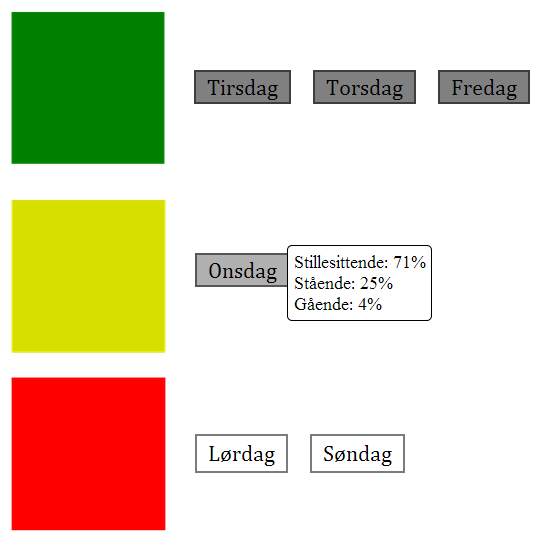
\includegraphics[width=0.5\textwidth]{u1Second.png}
  \caption[Second version of U1]{U1, the only overview chart in prototype 2.}
  \label{fig:uSecond}
\end{figure}

F2 was discarded and removed. The pictures from F2, illustrating the activity type, were added to the new version of F1, see Figure~\ref{fig:f1Second}. Changes made to F1 were not implemented, instead they were illustrated by an image file so that the planned changes could be shown to second focus group. The feedback on F3 was less concise, in the first focus group the participants expressed some concern that all the red in the visualization would be demotivating for the patients. We therefore changed the colour of sedentary activity from red to white, as seen in Figure~\ref{fig.f3Second}. One of the comments from the first focus group regarding aggregated charts was that nighttime distorted the visualizations, nighttime was therefore removed from the data set for these charts in prototype 2.

\begin{figure}[h!]
  \centering
  \begin{subfigure}[b]{0.45\textwidth}
    \centering
    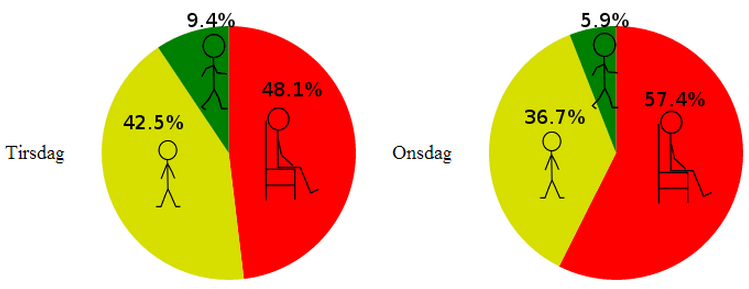
\includegraphics[width=\textwidth]{f1Second.png}
    \caption{F1}
    \label{fig:f1Second}
  \end{subfigure}
  \begin{subfigure}[b]{0.45\textwidth}
    \centering
    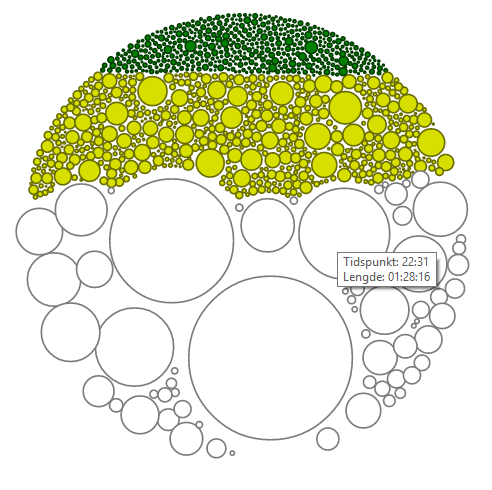
\includegraphics[width=\textwidth]{f3Second.png}
    \caption{F3}
    \label{fig:f3Second}
  \end{subfigure}
  \caption[Second version of F1 and F3]{Aggregated charts included in prototype 2.}
  \label{fig:aggCharts}
\end{figure}

T2 and T3 was discarded and removed. T1 was not changed other than the goal circle being appended to the right of each timeline, see Figure~\ref{fig:t1}. T4, see Figure~\ref{fig:t4}, received a colour change from red to white for sedentary activity, to further highlight actual activity. The inner radius of the hour-ticks, lines that marks each hour, was reduced to make the visualization look more like a normal clock. T5, see Figure~\ref{fig:t5}, was the only new visualization added. T5 uses stacked bars to show the activity level of each hour, and uses the goal circle to illustrate the patients activity compared to the goals set.

\begin{figure}[h!]
  \centering
  \begin{subfigure}[b]{0.6\textwidth}
    \centering
    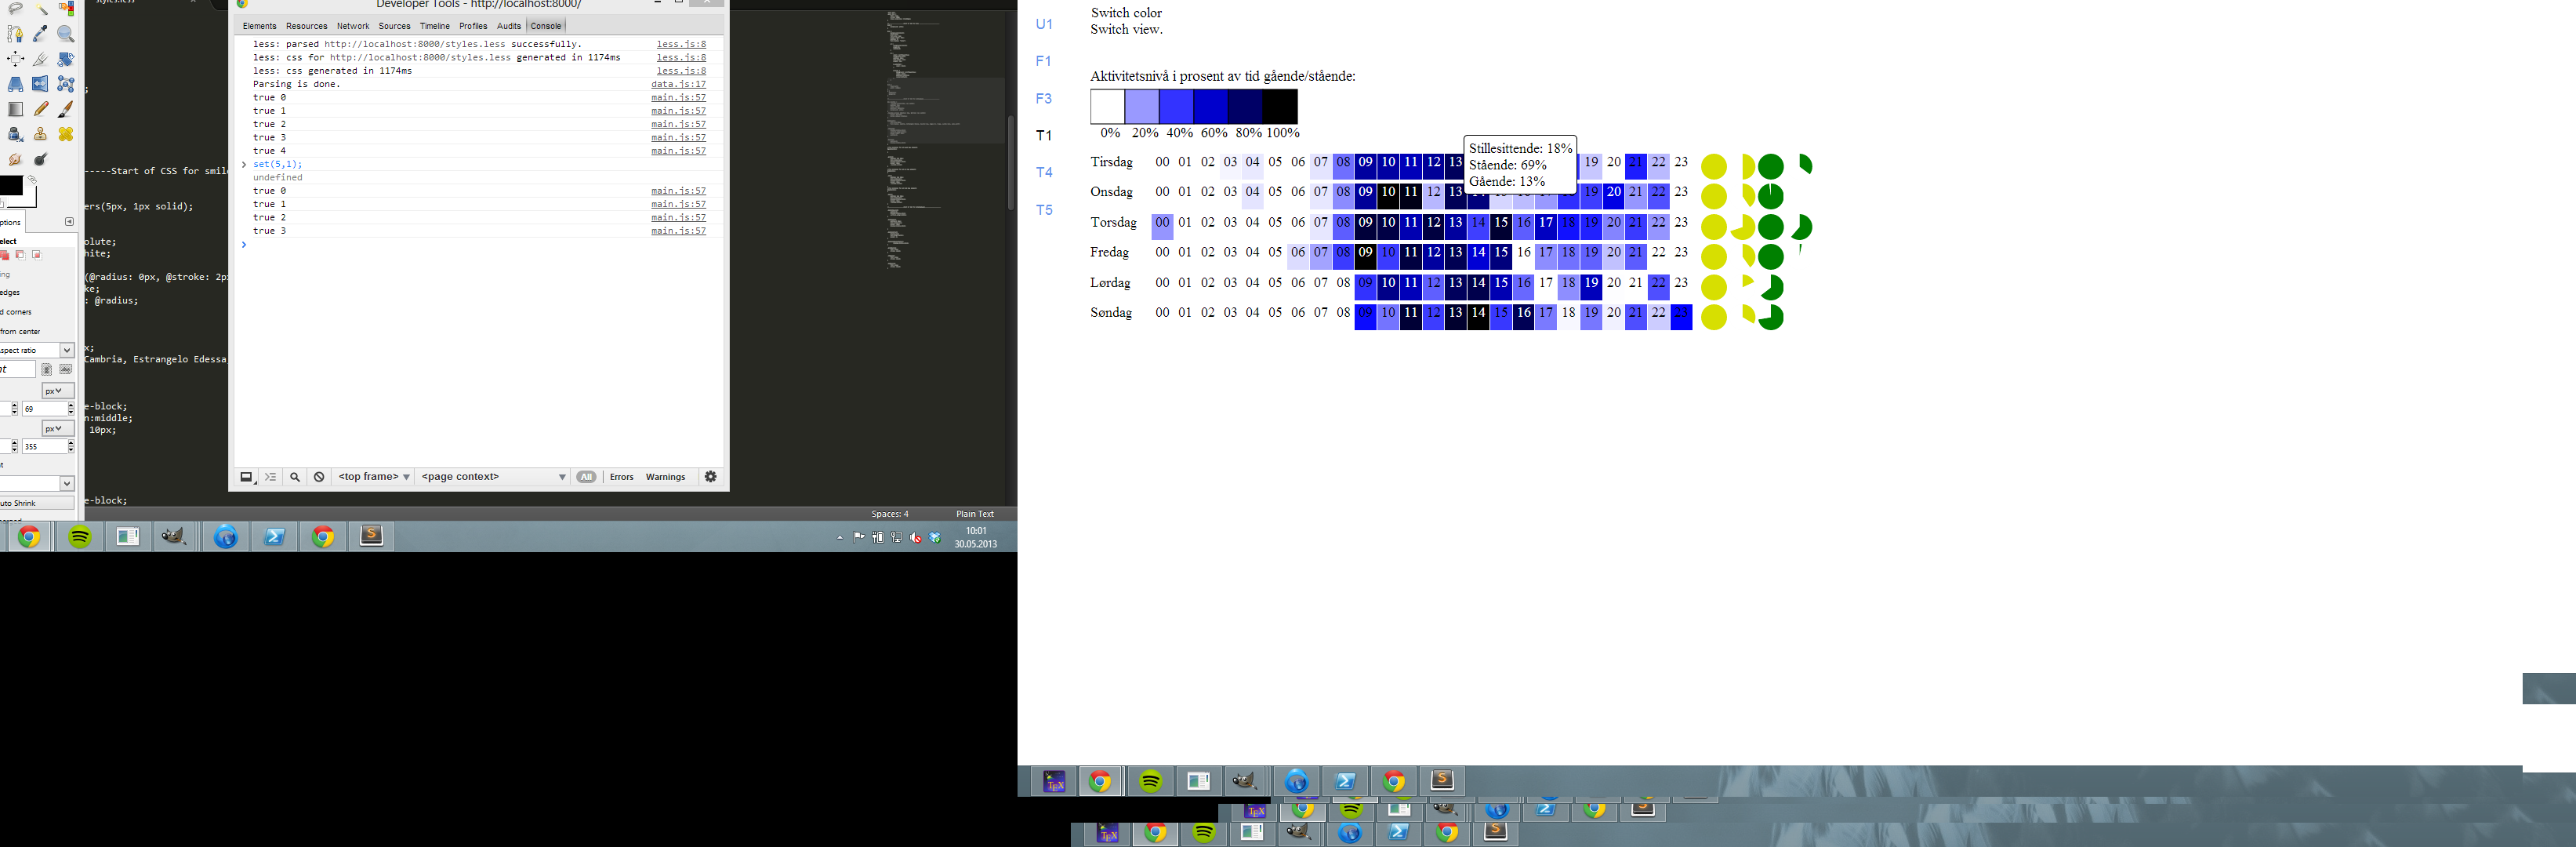
\includegraphics[width=\textwidth]{t1SecondWeek.png}
    \caption{T1}
    \label{fig:t1}
  \end{subfigure}
  \begin{subfigure}[b]{0.35\textwidth}
    \centering
    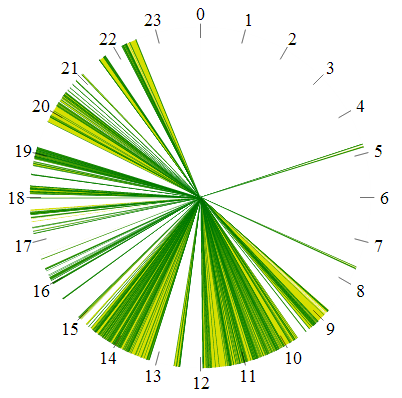
\includegraphics[width=\textwidth]{t4Second.png}
    \caption{T4}
    \label{fig:t4}
  \end{subfigure}
  \\
  \begin{subfigure}[b]{0.95\textwidth}
    \centering
    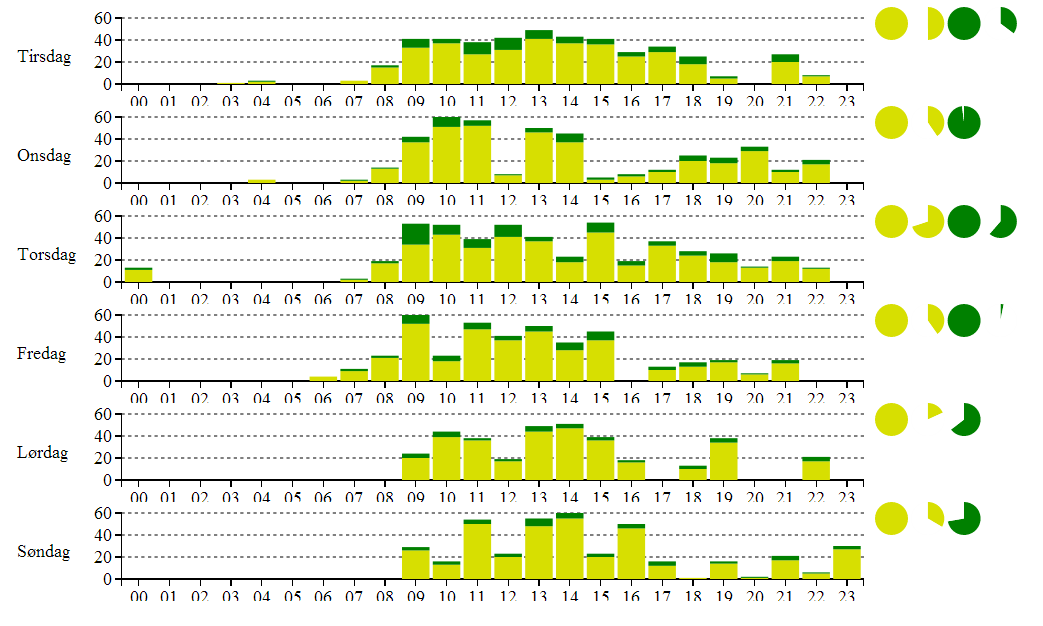
\includegraphics[width=\textwidth]{t5SecondWeek.png}
    \caption{T5}
    \label{fig:t5}
  \end{subfigure}
  \caption[Second version of T1, T4 and first version of T5]{Timeline charts included in prototype 2.}
\end{figure}

\chapter{Focus group 2}

\section{Procedure}


\subsection{Participants}
Participants from the previous focus group session, but due to conflicts in schedule only 4 out of the 5 could make it. For this session there were three females and one male present. The ages were between 34 - 36.

\subsection{Location and procedure}
The focus group was conducted at St. Olav's Hospital but we were unable to obtain the exact same room.  This mattered little because the room we did acquire had the all the necessary equipment. Much like the first session the participants were seated around a table facing a projector canvas. The visualizations were controlled by the assistant moderator, a laptop was provided for the participants at the end where they could shift through visualizations and colours, and discuss them in pairs of two. The entire session was once again video recorded and transcribed.

\subsection{Plan}
There were 3 main topics to be discussed during the focus group, the outline with explanations can be found below. The session ended with a summary and feedback on the focus group itself.

\begin{enumerate}
  \item Present the scenarios that the moderators had interpreted from last focus group.
  \item Let the participants validate, discuss and review the scenarios in written form.
  \item Present the revised visualizations while, and receive feedback on each before moving on to the next.
  \item Present the requirements created based on the feedback received in the previous focus group.
  \item Perform a group discussion and revision on the requirements.
  \item Perform an informal interview where the participants explain in detail how physiotherapy is practised by them.
\end{enumerate}

\section{Results}
% What should I say here my friend?

\subsection{Visualizations}
The second prototype had contained six visualizations, where five of them were modified versions of visualizations present in the first prototype and one was new. Other features that were added were the ability to set goals and a small chart, goal circle, for displaying how far the patient was from reaching his goal.

\subsubsection{Overview chart}
U1 was the only overview chart left after the changes made for the second prototype. The participants of the focus group liked the fact that the smilies had been replaced with coloured squares. They also liked the new functionality that gave them the ability to choose custom goals to be used in the classifications. One of the participants stated that: ``It is good that we can set the goals ourselves. How active different patients should be differs greatly.''. Another participants suggested adding the current goal to the visualization to make it easier to determine what each classification means. Most of the participants liked the simplicity of U1 and said that this was a type of diagram that many of their patients would understand, however one of the participants felt that the lack of detail in the diagram made it useless in practical situations.

Most of the participants like the new overview chart. The currently set goal should be displayed so it is clear how the what the classification means.

\subsubsection{Aggregated charts}
F2, the box diagram, was discarded in the second prototype, but the illustrations used to show each type of activity was added to F1. Nighttime was also remove, as requested in the first focus group. The participants were satisfied with the changes and liked the fact that the illustrations were now added to the pie chart, F1. All the participants agreed that the F1 was a good way to see the overall activity of the day, and that excluding nighttime increased the practical use of this chart.

F3 was not changed other than the colour for sedentary activity being white instead of red. The participants did not like the colour change particularly, and felt that the red would be better than white. All the participants agreed that this was a good way to visualize interval length. Some of the participants suggested that you should have the ability toggle nighttime on and off. They stated that nighttime is relevant for some patients that are active during the night, but for most patients nighttime just be in the way.

Both F1 and F3 were well received by the physiotherapists. F3 should have functionality for toggling nighttime on and off.

\subsubsection{Timeline and Clock}
T1 was the best liked visualization from focus group 1 and it was not changed much in the second prototype. Goal circle diagrams were added to each day to display how the patient's activity level compared to the goal set. The participants did not like the addition of the goal circles. One suggested being able to toggle the goal circles on and off, or be able to look at the goal circles as a separate visualization. As in U1 the participants felt that the current value of the goal should be displayed so that you knew what the circles represented.

T4 was not particularly well received in the first focus group, but it was added to the second prototype with a colour change of the sedentary activity from red to white. Even with the colour change the participants all agreed that this type of graph was too detailed and was not useful in practice. The visualization should be discarded.

T5 was the only new visualization added for prototype 2, if not counting the goal circles. Though this visualization was made on the request of the participants, they were not overly enthusiastic about T5. Most of the participants preferred T1 to T5. However when asked if they would like the option of having both visualizations available they all agreed that T5 could be useful in some cases and should be kept. Also here the participants felt that the goal circles made the chart overly complex, and that this should be a toggle option.

T4 should be removed as it has no practical use. T1 and T5 should be kept, but the user should be able to toggle the goal circles on and off. The current goal should be shown when the goal circles are displayed. 

\subsection{Colours and printouts}
Different colour choices were discussed with the participants. Because the projector did not tackle gradients well a laptop was used to show different colour choices. For the gradient colour the participants preferred white to blue to black, and white to black. For representing the different activity types (sitting, standing, walking) the participants liked red, yellow and green. One participant expressed some concern with the fact that red, yellow and green was used for sitting, standing and walking for F1, F3 and T5, but in U1 it was used for classifications. Using the same colours with different meanings can be confusing. An alternative to the coloured boxes in U1 should be found.

Because physiotherapists working for Trondheim Kommune do not have access to a colour printer, grayscale printouts were showed to the participants. The participants found it hard to T1 when printed because the printer did not handle grayscale gradients well. In this situation the participants preferred T5 over T1 since bars were used instead of colour for displaying the activity level. U1 and F1 was found to work well on printouts, however F3 was less useful when printed because the functionality to hold over a ball for more information about the interval is lost.

\subsection{Scenarios}
The scenarios crated after focus group 1 were reviewed in the second focus group. After discussing the scenarios with the participants we created a new version:
\vspace{-6mm}
\begin{enumerate}[itemsep=0cm, parsep=0cm]
\item When going analysing patients current activity level either individually or in cooperation with occupational therapists or other physiotherapists.
\item In communication with nursing homes and home care personnel.
\item In consultation with the patient.
\item In consultation with next of kin.
\item For educational purposes.
\end{enumerate}

Scenario 1 was changed to include occupational therapists. Occupational therapists are the colleagues that are most often consulted according to the physiotherapists. 

Scenario 2 was changed to include nursing homes as the most important partner to communicate with. Patients in nursing homes are in general much less active than those that live at home and there is therefore more need to inform the personnel working there about how inactive some of their patients are.

Scenario 3 was not changed. It is important to note that the physiotherapists estimated that maybe half of the patients would be cognitively capable of understanding the visualizations.

Scenario 4 was not changed.

Scenario 5 was a new scenario added on the request of the focus group. An increasing part of their work consists of tutoring home care personnel about exercises that patients can perform to increase their activity. The participants felt using visualizations in this setting would be useful. 

\subsection{Requirements}
% What should I write here, if I recall correctly the requirements were not changed. What should we do? Should we crate some more specific requirements? It feels a little strange to just leave the same requirements here as the ones we had after focus group 1.

\begin{table}[h!]
  \begin{center}
  \begin{tabular}{|c|p{12cm}|}
    \hline
      \textbf{Id} & \textbf{Requirement} \\ \hline
    \multicolumn{2}{|l|}{The visualizations should \ldots} \\ \hline
      F2-1 & give the user an overview of the week where the days are classified by national or personal goals \\ \hline
      F2-2 & show the activity level for each hour of the day \\ \hline
      F2-3 & make it simple to identify periods of inactivity \\ \hline
      F2-4 & make it possible to compare multiple days \\ \hline
      F2-5 & make it easy to identify hours of the day where activity can be added \\ \hline
      F2-6 & show the activity level compared to national or personal goals \\ \hline
      F2-7 & let the user identify patients that are active during the night \\ \hline
      F2-8 & let you compare two separate weeks to see the patients progress \\ \hline
      F2-9 & should be printable in grayscale \\ \hline
  \end{tabular}
  \end{center}
  \caption{Functional requirements from the second focus group}
\end{table}

\begin{table}[h!]
  \begin{center}
  \begin{tabular}{|c|p{12cm}|}
    \hline
      \textbf{Id} & \textbf{Requirement} \\ \hline
    \multicolumn{2}{|l|}{The visualizations should \ldots} \\ \hline
      F2-10 & not be judgemental towards the patients activity level \\ \hline
      F2-11 & should be honest about the patients activity level \\ \hline
      F2-12 & should motivate the patient to be more active \\ \hline
      F2-13 & should be intuitive and easy to understand and explain to the user \\ \hline
  \end{tabular}
  \end{center}
  \caption{User experience requirements from the second focus group}
\end{table}



\subsection{Physiotherapy in practice} 
To get an overview of how physiotherapy is conducted in Norway we performed an interview on the participants of the focus group. The physiotherapists that were recruited for the focus groups work with elderly and patients that otherwise needs to be helped from home (e.g. patients suffering from Cerebral Palsy). The seven step process below describes what happens when a patient is referred to a physiotherapist:

\vspace{-4mm}
\begin{enumerate}
  \item A general practitioner or other healthcare personnel can fill out an application for their patients to see a physiotherapist.
  \item The application is then evaluated and placed into a priority queue. Applications may be prioritized if the matter is time sensitive, such as recovery after a fracture or surgery.
  \item When a physiotherapist is available they are given the application on top of the priority queue.
  \item The physiotherapist then makes a house visit to the patient so that they may get an understanding of the current activity level. The activity level is mapped through several different types of exercises and through conversations with the patient. Overall posture and the speed of movements help assess the general state of the patient.
  \item The next step is to create an exercise plan for the patient in order to increase the activity level. During conversations with the patient the physiotherapist discusses what kind of improvements are realistic to achieve considering the current activity level, motivation, physical health etc. All of this data is then used to create an exercise plan that the patient can follow to reach their goals.
  \item When an appropriate plan has been created the physiotherapist returns to the patient to explain how the exercises are executed as well as motivating the patient to reach his goals. The plan may also include other types of activity, for many patients something as simple as walking to the store to buy groceries can be enough to make a difference in the overall activity.
  \item Physiotherapist will return regularly to check up on the patient. The interval between check-ups will vary in respect to how well the physiotherapists expects the patient to follow the agreed upon plan. Some patients lack motivation, and will need more regular check-ups. During such meetings the physiotherapist will get an idea of how much the patient has improved, emphasizing the improvement made is an important factor in motivating the patient to abide to the plan. If there has been little or no change in the activity level, the physiotherapist may want to make changes to the plan so better results are achieved.
\end{enumerate}

\section{Interpretation}

\chapter{Discussion}
{\Large Not yet reviewed internally}
\section{Use Cases: Scenarios and User Group}
%Skrive om hvilken visualizering som er bra til hvilket scenario. Skrive om hvordan vi kom frem til scenarioene og at de kom med mange scenarioer vi ikke tenkte p�, i tillegg til at ikke alle visulizeringene egnet seg til alt.
Our first research question states:
\begin{quote}
\textit{What are the relevant use cases for visual presentation of the accelerometer data in physical therapy, form the physiotherapist's perspective?}
\end{quote}

Initially we designed the first prototype for two scenarios:
\begin{table}[h!]
  \begin{tabular}{|c|p{10cm}|}
    \hline
    \textbf{Id} & \textbf{Scenario} \\ \hline
    IS-1 & Mapping the activity level of patients \\ \hline
    IS-2 & In consultation with patients \\ \hline
  \end{tabular}
  \caption{Table showing the initial scenarios.}
\end{table}

These are the most obvious scenarios for the system. After the first and second focus group three more scenarios emerged, as well as the initial ones being heavily modified:

\begin{table}[h!]
  \begin{tabular}{|c|p{10cm}|}
    \hline
    \textbf{Id} & \textbf{Scenario} \\ \hline
    S2-1 & When analysing patients activity level, either individually or in cooperation with occupational therapists or other physiotherapists. \\ \hline
    S2-2 & In consultation with the patient. \\ \hline
    S2-3 & In communication with nursing homes and home care personnel. \\ \hline
    S2-4 & In consultation with next of kin. \\ \hline
    S2-5 & For educational purposes. \\ \hline
  \end{tabular}
  \caption{Table showing the scenarios after the second focus group.}
\end{table}

The first scenario was changed to include the cooperation with other physiotherapists or occupational therapists. During the second focus group the participants informed us that if they were to discuss a patient with colleagues it would usually be with an occupational therapist or in rare cases another physiotherapist. Normally the physiotherapists would not consult their colleagues about specific patients. 

The second scenario is one of the most important uses the system has. Showing the visualizations to the patient can be useful in many cases, for example when explaining to the patient their current activity level, and why exercise or more movement is needed. Visualizations are also useful when motivating the patients, by showing them detailed figures of how they are progressing. Many of the patients that are treated by the physiotherapists who working for Trondheim Kommune are elderly and not as cognitively capable as they once were, especially those living in nursing homes. During the second focus group we asked the participants how many percentage of their patients they thought would be capable of understanding the visualizations, their estimate was 50\%. Of course some of the visualizations are very simple and could probably be used for a larger patient group, but less detailed visualizations will often be less helpful. 

For patients that can not understand the visualizations themselves, scenario 3 and 4 become increasingly important. Patients living in nursing homes receive helps continuously through the day, and are unable to preform trivial tasks like making breakfast or go shopping. During the focus groups the participants were concerned that when patients stopped doing such tasks the little activity previously had was lost, leading to an inactive and unhealthy lifestyle. To combat this, the participants were eager to be able to monitor the activity of such patients and in cooperation with personnel working there increase the activity of the patient. 

In many cases the patients next of kin can be consulted after or during evaluation of the patients activity level. Next of kin can be an important motivator for the patient, and help the physiotherapists persuade patients to follow the agreed upon treatment plan. Next of kin are normally interested in the well being of the patient. The system can be used to help them get a picture of the overall activity level of the patient as well as how they are progressing if they have started treatment. In cases where the patients are not capable of understanding the visualizations themselves, it can be helpful to show them to the next of kin to give them an idea of what needs to be done to get to an acceptable level of activity. Next of kin are able to spend more time with the patient than the physiotherapists and can thus help the patient achieve their goals by motivating them to take a walk or perform household tasks.

% This last part was probably a little strange, but I was very uncertain as what to write here. 
The focus group participants believed that the visualizations could be helpful for educational purposes. A project currently ongoing in Trondheim is teaching home care personnel how to preform physiotherapy exercises with their patients. This will give elderly patients living at home better access to help when they have been asked to preform exercises by the physiotherapists. The participants of the focus groups suggested that visualizations could be used in training of both physiotherapy students and home care personnel to show them how preforming different exercises can help improve the overall activity of the patient.

\section{Requirements}
The second research question states:
\begin{quote}
\textit{What are the functional and user experience requirements for visualizations of accelerometer data in scenarios identified by the physiotherapists?}
\end{quote}

Requirements gathering is an important part of any software development project. Because the initial requirements were created in cooperation with a domain expert and not the participants of the focus groups we saw a lot of changes to the requirements after the first focus group. The requirements are supposed to give instructions as to what types of visualizations should be created, and with all the feedback and changes to the visualizations after focus group 1 it is not surprising that the requirements also changed substantially.

\begin{table}[h!]
  \begin{center}
  \begin{tabular}{|c|p{12cm}|}
    \hline
      \textbf{Id} & \textbf{Requirement} \\ \hline
    \multicolumn{2}{|l|}{The visualizations should \ldots} \\ \hline
      IR-1 & give an overview of the week \\ \hline
      IR-2 & give a summary of the daily activity \\ \hline
      IR-3 & show the activity level for each hour of every day \\ \hline
      IR-4 & let you compare hours from multiple days \\ \hline
      IR-5 & show the activity level for each minute of every day \\ \hline
      IR-6 & let you compare minutes from multiple days \\ \hline
      IR-7 & let the user identify patients that are active during the night \\ \hline
  \end{tabular}
  \end{center}
  \caption{Initial requirements.}
  \label{tab:initReq}
\end{table}

Looking at initial requirements in table~\ref{tab:initReq}, requirements IR-5 and IR-6 were removed after talking to the physiotherapists in focus group 1. Visualizations showing the continuous activity pattern of users was seen as too detailed to be useful. The participants also felt that it was too hard to see the activity, because it was hidden by the inactive and standing periods. The other initial requirements were modified and rephrased, but still remain in the R1-version of the requirements, see table~\ref{tab:f1Req}. 

Requirement R1-5 is a direct results of comments from the participants during the first focus group. They stated that one of the most useful features of the system is the ability to see when during the day the patient are inactive. This can be used to plan activity and exercises to specific hours of the day when the physiotherapists knows the patient will most likely be inactive. Having this type of detailed information can help the physiotherapists create an even more specific treatment plan for the patient, and possibly increasing the quality and effectiveness of the treatment. A functionality that was requested during the first focus group was the ability to set goals. The physiotherapists had a hard time identifying whether the patients data represented an active or an inactive person without comparing the data to some fixed goal. To satisfy this request R1-6 was a new requirement added after focus group 1. IR-1 was also changed to R1-1 to make the classification in the overview charts take into consideration patient goals.

Another interesting addition was R1-9, which states that the visualizations should be have printable greyscale versions. It was surprising to hear about how few technological aids were available to the physiotherapists working for Trondheim Kommune (municipality of Trondheim). For scenarios where the physiotherapists only have access to grayscale printouts, important system functionality such as interactivity, will be lost.

\begin{table}[h!]
  \begin{center}
  \begin{tabular}{|c|p{12cm}|}
    \hline
      \textbf{Id} & \textbf{Requirement} \\ \hline
    \multicolumn{2}{|l|}{The visualizations should \ldots} \\ \hline
      R1-1 & give the user an overview of the week where the days are classified by national or personal goals \\ \hline
      R1-2 & show the activity level for each hour of the day \\ \hline
      R1-3 & make it simple to identify periods of inactivity \\ \hline
      R1-4 & make it possible to compare multiple days \\ \hline
      R1-5 & make it easy to identify hours of the day where activity can be added \\ \hline
      R1-6 & show the activity level compared to national or personal goals \\ \hline
      R1-7 & let the user identify patients that are active during the night \\ \hline
      R1-8 & let you compare two separate weeks to see the patients progress \\ \hline
      R1-9 & be printable in grayscale \\ \hline
  \end{tabular}
  \end{center}
  \caption{Functional requirements from the first focus group}
  \label{tab:f1Req}
\end{table}

Two requirements were added after the second focus group, F2-15 and R2-16, see table~\ref{tab:f2Req}. R2-15 is a clarification of the first requirement. The participants felt that there was no requirement specifying the need for aggregated charts, and R2-15 was therefore added. Another functionality that was requested was the ability to toggle nighttime on and off. In the first focus group many of the participants felt that including nighttime, especially in the aggregated charts, made the inactive part of the chart too large. Nighttime was therefore removed for some of these graphs in the second prototype. However, the participants were now uncertain as to what period of the night had been removed. It was therefore suggested that that the user should be able to toggle nighttime on and off, so that in cases where it would be helpful to see the entire dataset this option would still be available. The participants also wanted the ability to define the time interval that should be considered  nighttime. For patients living in institutions nighttime is similar for all the patients, but for patients living at home nighttime might differ from patient to patient.

\begin{table}[h!]
  \begin{center}
  \begin{tabular}{|c|p{12cm}|}
    \hline
      \textbf{Id} & \textbf{Requirement} \\ \hline
    \multicolumn{2}{|l|}{The visualizations should \ldots} \\ \hline
      R2-1 & give the user an overview of the week where the days are classified by national recommendations or personal goals \\ \hline
      R2-2 & show the activity level for each hour of the day \\ \hline
      R2-3 & make it easy to identify the length of activity intervals \\ \hline
      R2-4 & make it possible to compare multiple days \\ \hline
      R2-5 & make it easy to identify hours of the day where activity can be added \\ \hline
      R2-6 & show the activity level compared to national or personal goals \\ \hline
      R2-7 & let the user identify patients that are active during the night \\ \hline
      R2-8 & let you compare two separate weeks to see the patients progress \\ \hline
      R2-9 & should be printable in grayscale \\ \hline
      R2-15 & show the activity distribution for a day (sedentary, standing, walking) \\ \hline
      R2-16 & allow the users to toggle if nighttime should be included or not \\ \hline
  \end{tabular}
  \end{center}
  \caption{Functional requirements from the second focus group}
  \label{tab:f2Req}
\end{table}

\begin{table}[h!]
  \begin{center}
  \begin{tabular}{|c|p{12cm}|}
    \hline
      \textbf{Id} & \textbf{Requirement} \\ \hline
    \multicolumn{2}{|l|}{The visualizations should \ldots} \\ \hline
      F2-10 & not be judgemental towards the patients activity level \\ \hline
      F2-11 & should be honest about the patients activity level \\ \hline
      F2-12 & should motivate the patient to be more active \\ \hline
      F2-13 & should be intuitive and easy to understand for the user and third parties \\ \hline
      F2-14 & be easy to explain to cognitively capable patients \\ \hline
  \end{tabular}
  \end{center}
  \caption{User experience requirements from the second focus group}
  \label{tab:f2ReqUx}
\end{table}

Talking with the physiotherapists also gave us the ability to explore \gls{ux} requirements for the system, see table~\ref{tab:f2ReqUx}. The \gls{ux} requirements we created are important to keep in mind when creating requirements that may not be intuitive without understanding how the physiotherapists work. One of the first responses we got when going through the visualizations in the first focus group, was that the visualization had a negative attitude. For example using smilies to represent the classifications could demotivate and be judgemental towards the patient. These are issues we did not consider when first creating prototype 1. The physiotherapists also stressed that though the visualizations should not be judgemental it was just as important that they did not lie. They should give the patient an honest representation of their activity level, but without making the patient feel hopeless. Many patients are prone to give up before they have even started, and it is paramount that the visualizations do not contribute in discouraging the patient.

Motivating patients is another important \gls{ux} requirements. One of the physiotherapists pointed out that patients like to see quantitative data to show that they are improving. Progress can be slow and hard to notice from day to day. This can in many cases discourage patients from doing their exercises. Seeing quantitative proof that you are constantly improving can be a powerful motivational tool, as it gives the patient a reward for following the exercise plan. One of the physiotherapists also stated that patients tend to trust more in statistics and diagrams than they do in the qualitative judgement from the physiotherapists alone. Using visualizations in their work can therefore help them persuade patients who are otherwise distrustful or feel that the treatment plan is ineffective or pointless. For the patients to be motivated by the visualizations, they need to be able to understand them, and this is covered by the R2-12 requirement. 

\section{Visualization}
\begin{quote}
  \textit{What are the preferred visualizations by the physiotherapists for the scenarios and requirements?}
\end{quote}

During the creation of the first paper sketches we created three groups of visualizations: overview charts, aggregated charts and timeline charts. The overview charts were designed to let the user to quickly get an overview of the week as a whole. For the first prototype two such overviews were created U1 and U2. U2 was quickly discarded because it contained too many details which only confused the participants of the first focus group. U1 was kept in the second prototype and received positive feedback by the participants in the second focus group. U1 uses personal or national goals to classify each day into one of three categories. Making U1 very easy to understand, and one of the physiotherapists stated that because it was so easy to understand this might be one of the visualizations that would be shown to the patients. The visualization also works well for printouts, both colour and grayscale. To further improve U1 an indication as to what the current goal is set to should be added, such information would help the physiotherapist and patient understand what the different classifications corresponds to.

The aggregated charts summed up the day to show the distribution of different types of activity. Initially there were three types of aggregated charts: F1, F2 and F3. F1 and F2 were combined for the second prototype to become a standard pie chart with three slices, one for each activity type. The pie chart also contains illustrations that show what type of activity each slice corresponds to. Pie charts are easy to understand because most people will have seen them before, know what they mean and know how to read them. F1 can therefore also be shown to the patient when explaining their current level of activity. F3 is a bubble chart, most people will not have seen this type of chart before and it is not as intuitive as F1. The physiotherapists like the chart because you could use it to see intervals of activity, for example what was the longest walk the patient took during the day. This type of graph would most likely not be shown to the patients as most of them would not understand it. F3 could be used in communication with nursing homes and home care personnel, for example if the patient needs to be walking for longer periods of time not just in small intervals. 

Timeline charts show the activity during the day continuously or in aggregated blocks. Four timeline charts were initially created prototype: T1, T2, T3 and T4. T2, T3 and T4 showed activity during the day minute for minute without condensing it into hours. These visualizations were discarded because the physiotherapists felt that the amount of detail was unnecessary and only made the visualizations harder to read and less useful. T1 uses 24 blocks where the activity of each hour were aggregated and displayed using a gradient. T1 was the preferred graph, as it was easy to get an overview of the day as a whole, as well as the entire week by stacking many days on top of each other. This meant that the physiotherapists could easily get an overview of the overall activity pattern of the patient. This made it easy to find inactive hours where the patient could be motivated to do exercises or move around. Noticing patients who are active during the night is also easy due to the way hours with activity gain increase in colour intensity. During the focus group one of the physiotherapists told us that a common problem for elderly patients is that they can not sleep and therefore walk around during the night, leading to less activity during the day. Such patterns can easily be detected using T1, as an example we were able to see from the example data that the patient would walk for a few minutes every night at 4 am, probably to go to the toilet. 

Though the T1 is not very hard to understand,  but it requires more understanding than U1 and F1, therefore it could most likely only be displayed to the most cognitively capable patients. Another issue with T1 is that the gradient colours it uses do not translate well when printed. T5 was created for the second prototype and like T1 divides the day into 24 blocks, but instead of using gradient to display the distribution of activity stacked bars are used. This visualization is also similar to the chart used in the activPAL software, but in T5 seated or lying activity is not displayed with bars, this increases the readability of the graph. Despite this T1 was still the favourite because it is easier to stack days on top of each other when using gradient colouring instead of stack bars to represent activity within an hour. One benefit of T5 compared to T1 is that is works much better when printed because it does not use a colour gradient, but bars to show the amount of activity.

For the second prototype personal and national goals were added. This addition was heavily requested by the physiotherapists after the first focus group. To show how the patient's activity compared to the goals that had been set, a visualization called goal circles was created. As the name suggests the visualization uses circles to display how far the patient is from reaching the goal or how far they have exceeded it. The goal circles were appended to each day of T1 and T5. The participants of the second focus group did not like this, and felt that the goal circles should have been its own visualization, used only to see if the patient were reaching the goals set. The goal circles are also intuitive and easy to understand, and they could be shown to some patients. An issue with the goal circles is that they do not display the currently set goals, all graphs using the goals should display what the current goals are set to. Goals are an important motivational factor when patients are attempting to become more active.

Table~\ref{tab:reqSat} shows which requirements are satisfied by each visualization. Each row represents a visualization and each column corresponds to a functional requirement. A -- means that the requirement is not satisfied by the visualization and a + means that it is satisfied. As we can see there are two requirements, R2-8 and R2-16, that are not covered by any of the visualizations. R2-8 says that you should be able to compare two different weeks to see if there has been progress. Comparing weeks is important for the system to function as a motivative tool. This requirement was suggested after focus group 1, but was not implemented due to lack of time. R2-16 states that the visualizations should let you toggle nighttime on and off. This requirement was suggested in focus group 2 and was therefore not implemented for prototype 2.covered by any of the visualizations. R2-8 says that you should be able to compare two different weeks to see if there has been progress. Comparing different weeks is important for the system to function as a motivational tool. This requirement was suggested after focus group 1, but was not implemented due to lack of time. R2-16 states that the visualizations should let you toggle nighttime on and off. This requirement was suggested in focus group 2 and was therefore not implemented for prototype 2.

\begin{table}[h!]
  \centering
  \begin{tabular}{|c|c|c|c|c|c|c|c|c|c|c|c|}
    \hline
    & R2-1 & R2-2 & R2-3 & R2-4 & R2-5 & R2-6 & R2-7 & R2-8 & R2-9 & R2-15 & R2-16 \\ \hline
    U1 & + & -- & -- & + & -- & -- & -- & -- & + & -- & -- \\ \hline
    F1 & -- & -- & -- & + & -- & -- & -- & -- & + & + & -- \\ \hline
    F3 & -- & -- & + & -- & + & -- & -- & -- & -- & + & -- \\ \hline
    T1 & -- & + & -- & + & + & + & + & -- & -- & -- & -- \\ \hline
    T5 & -- & + & -- & + & + & + & + & -- & + & -- & -- \\ \hline
  \end{tabular}
  \caption{Table showing which requirements each visualization satisfies.}
  \label{tab:reqSat}
\end{table} 

Table~\ref{tab:scenSet}, see below, shows which visualizations satisfy each scenario. The first scenario is physiotherapists using the visualizations to analyse the patients activity level. In such cases all the visualizations can be utilized to get the best overview of the patients activity situation. For the most part T1 and T5 would be used as these give the best overview of the week and it is easy to identify where more activity can be added. 

\begin{table}[h!]
  \centering
  \begin{tabular}{|c|c|c|c|c|c|}
    \hline
       & S2-1 & S2-2 & S2-3 & S2-4 & S2-5 \\ \hline
    U1 & +  & +  & -- & +  & +  \\ \hline
    F1 & +  & +  & +  & +  & +  \\ \hline
    F3 & +  & -- & +  & -- & +  \\ \hline
    T1 & +  & -- & +  & -- & +  \\ \hline
    T5 & +  & +  & +  & +  & +  \\ \hline
  \end{tabular}
  \caption{Table showing which scenarios each visualization satisfies.}
  \label{tab:scenSet}
\end{table}

The second scenario is using the visualizations in consultation with the patient. For many of the patients it will not be possible to show any of the visualizations, but for those that are cognitively capable most of the visualizations can be used. F3 was excluded because it can be hard to explain, and it does not contain information that is critical to convey to the patient. T1 will not work on paper printouts, but could be used if the physiotherapists have access to laptops or touch pads.

The third scenario is concerned with communication with nursing homes and home care personnel. All visualizations can be used for this purpose, but U1 will probably not be effective in conveying much information of interest and was therefore excluded. F3 and T1 will can be helpful tools when discussing the activity level of patients with other health care personnel.

Consulting the next of kin is the fourth scenario. Most visualizations can be used for this purpose. F3 was excluded because it will probably be more confusing than helpful in explaining the patients current activity level. T1 was also excluded as it will does not work well for printouts.

For educational purposes, scenario 5, all the visualizations can be used. Each visualization serves different functions and to get a complete overview of the patients activity level it can be useful to look at multiple visualizations. T1 and F1 are probably the best for this purpose. F3 can be used in situations where it is helpful to see the length of different type of activity.

\chapter{Analysis of Research methods}
%Tror jeg ``forsvarer'' for mye, burde bare skrive alt vi har gjort feil uten å gjøre no mer kanskje.
Vi burde kanskje omformulere denne seksjonen til "Analysis of research methods" eller noe sånt?


\section{Initial requirements interview}
%Jeg er litt redd for å kalle dette et interview som vi gjør. fordi det var jo egentlig ikke det. Hvis vi først skriver at det var et intervju burde vi i såfall ha skrevet noe om det i HCI kapitellet, som vi kan referere til og hvorfor det skader validiteten. Skal vi heller si ``talks''?
The initial requirements were gathered through informal and casual interviews with a physiotherapist conducting a research project at St. Olav's Hospital. There was also no structure to the interview. The individual did not work in direct contact with patients, and the data is primarily used in communication with other healthcare personnel. 
%Kanskje ta ut denne biten og heller putte det inn i initial requirements?
They did however have a great deal of experience with visual representations of such data, and communicating through the use of such visual aids.

Due to the background of the interview subject we might not have covered requirements that address concerns when presenting the visualizations in consultation with a patient. 
%Fjerne kanskje denne biten her, der er et ``forsvar''
However we believe that some of these concerns were addressed through additional requirements that arose during the focus group sessions.

%Tror kanskje jeg forsvarer for mye mot slutten, burde kanskje bare konstantere.
\section{Focus group}
Nielsen states that the focus group should have at least six participants. We had originally invited 6, but only 5 were able to attend the sessions. We had no issues with keeping the discussion flowing and the participants were all quite forward when they saw something they disliked. We were unable to represent all the relevant user groups as the participants only represented state employed therapists that visited patients at their residence. We have not taken into account physiotherapists that have office hours or work in the private sector.

We deliberately chose to control the navigation through the visualizations ourselves during the focus group, even though Nielsen mentions this as one of two pitfalls that may occur in a focus group. He specifies that by using a demo the user will never have to consider the meaning of screen options or what to do next. In our case the prototype is not an application with intractable buttons, but the prime focus are the visualizations themselves. 

A possible mistake might have been to give a short description of the visualizations to the participants, rather than letting them figure it out on their own, in order to verify if they were intuitive enough. Providing them with a mouse to test the interactivity themselves might have been more beneficial.

\section{Paper Sketches and Prototype}
A mistake we identified once the first focus group was conducted was that we should have worked harder to involve potential users while creating paper sketches. ISO 9241-210 states that one should make an effort to involve users in every step of the development, we failed to do so and the consequences of this have become apparent. If we had presented paper sketches to the users we could have perhaps avoided spending time and resources to create high fidelity prototypes of visualizations that would be quickly discarded.
\chapter{Conclusion}
%\item[Research Question 2:] What are the functional and user experience requirements for visualizations of \gls{imu} data in scenarios identified by the physiotherapists?

\section{RQ1: User Scenarios}


\begin{enumerate}[itemsep=0cm, parsep=0cm]
\item When analysing patients activity level, either individually or in cooperation with occupational therapists or other physiotherapists.
\item In consultation with the patient.
\item In communication with nursing homes and home care personnel.
\item In consultation with next of kin.
\item For educational purposes.
\end{enumerate}


\section{RQ2: Requirements}
The requirements have had several iterations through the project. It started with the initial requirements outlined in chapter~\ref{ch:initialRequirements} which were iterated upon in focus groups 1 (chapter \ref{ch:focusGroup1}). In addition a set of \gls{ux} requirements were outline after focus group 1. Table~\ref{tab:f2ReqCon} and~\ref{tab:f2ReqUxCon} display what we consider to be the final functional and \gls{ux} requirements for visualizations of data identified by the physiotherapists.
\begin{table}[h!]
  \begin{center}
  \begin{tabular}{|c|p{12cm}|}
    \hline
      \textbf{Id} & \textbf{Requirement} \\ \hline
    \multicolumn{2}{|l|}{The visualizations should \ldots} \\ \hline
      F2-1 & give the user an overview of the week where the days are classified by national recommendations or personal goals \\ \hline
      F2-2 & show the activity level for each hour of the day \\ \hline
      F2-3 & make it easy to identify the length of activity intervals \\ \hline
      F2-4 & make it possible to compare multiple days \\ \hline
      F2-5 & make it easy to identify hours of the day where activity can be added \\ \hline
      F2-6 & show the activity level compared to national or personal goals \\ \hline
      F2-7 & let the user identify patients that are active during the night \\ \hline
      F2-8 & let you compare two separate weeks to see the patients progress \\ \hline
      F2-9 & should be printable in grayscale \\ \hline
      F2-10 & show the activity distribution for a day (sedentary, standing, walking) \\ \hline
      F2-11 & allow the users to toggle if nighttime should be included or not \\ \hline
  \end{tabular}
  \end{center}
  \caption{Functional requirements from the second focus group}
  \label{tab:f2ReqCon}
\end{table}

Both functional and UX requirements presented here should be used as a basis for creating visualizations in physiotherapy. We assume that these requirements will be expanded upon when developing a system for a specific customer and purpose.

\begin{table}[h!]
  \begin{center}
  \begin{tabular}{|c|p{12cm}|}
    \hline
      \textbf{Id} & \textbf{Requirement} \\ \hline
    \multicolumn{2}{|l|}{The visualizations should \ldots} \\ \hline
      F2-11 & not be judgemental towards the patients activity level \\ \hline
      F2-12 & should be honest about the patients activity level \\ \hline
      F2-13 & should motivate the patient to be more active \\ \hline
      F2-14 & should be intuitive and easy to understand for the user and third parties \\ \hline
      F2-15 & be easy to explain to cognitively capable patients \\ \hline
  \end{tabular}
  \end{center}
  \caption{User experience requirements from the second focus group}
  \label{tab:f2ReqUxCon}
\end{table}

\section{Further work}




\renewcommand*{\bibname}{References}
\bibliographystyle{unsrtnat}
\bibliography{main}

% Uncomment the following if you have any appendix
 \appendix
 \addtocontents{toc}{%
  \protect\vspace{1em}% 
  \protect\noindent \bfseries \appendixtocname\protect\par
  \protect\vspace{-.5em}%
 }
 \renewcommand{\chaptername}{\appendixname}
% include below possible appendices (chapters)
\chapter{CSV Document}
\label{csvDocument}

\begin{figure}[h!]
	\centering
		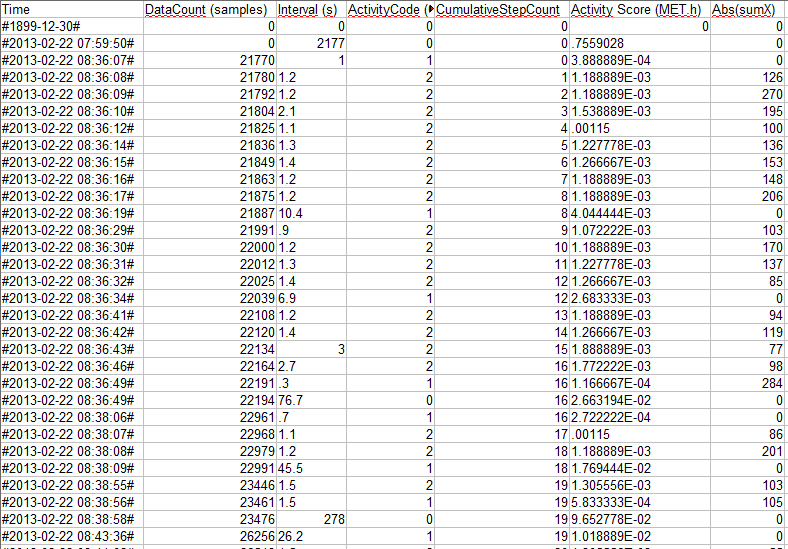
\includegraphics[width=1\textwidth]{csv.png}
		\caption[CSV Document]{The CSV document as seen in Libre Calculator}
		\label{fig:csvExtract}
\end{figure}

\begin{table}[h!]
  \centering
  \begin{tabular}{|l|p{8.4cm}|}
    \hline
    \textbf{Row Title} & \textbf{Description} \\ \hline
    Time & Time when the state started. \\ \hline
    DataCount & The amount of sensor readings the event interval is based on (not used in this project). \\ \hline
    Interval & Duration for the event interval presented in seconds. \\ \hline
    ActivityCode & Represents the activity of the user either sedentary (0), standing (1), or walking (2). \\ \hline
    CumulativeStepCount & The total amount of steps taken since movement tracking was started (not used in this project). \\ \hline
    Activity Score & Activity score rating (not used in this project) \\ \hline
    Abs(sumX) & Acceleration intensity (not used in this project). \\ \hline
  \end{tabular}
  \caption[CSV row explanation]{A short description of the rows in figure~\ref{fig:csvExtract}.}
  \label{tab:csvDescription}
\end{table}

\chapter{Checklist}
\label{checklist}
A copy of the checklist the physiotherapists have to go through when mapping patients health and activity level is located in this appendix. Unfortunately it is in Norwegian and there was not enough time to translate it. 
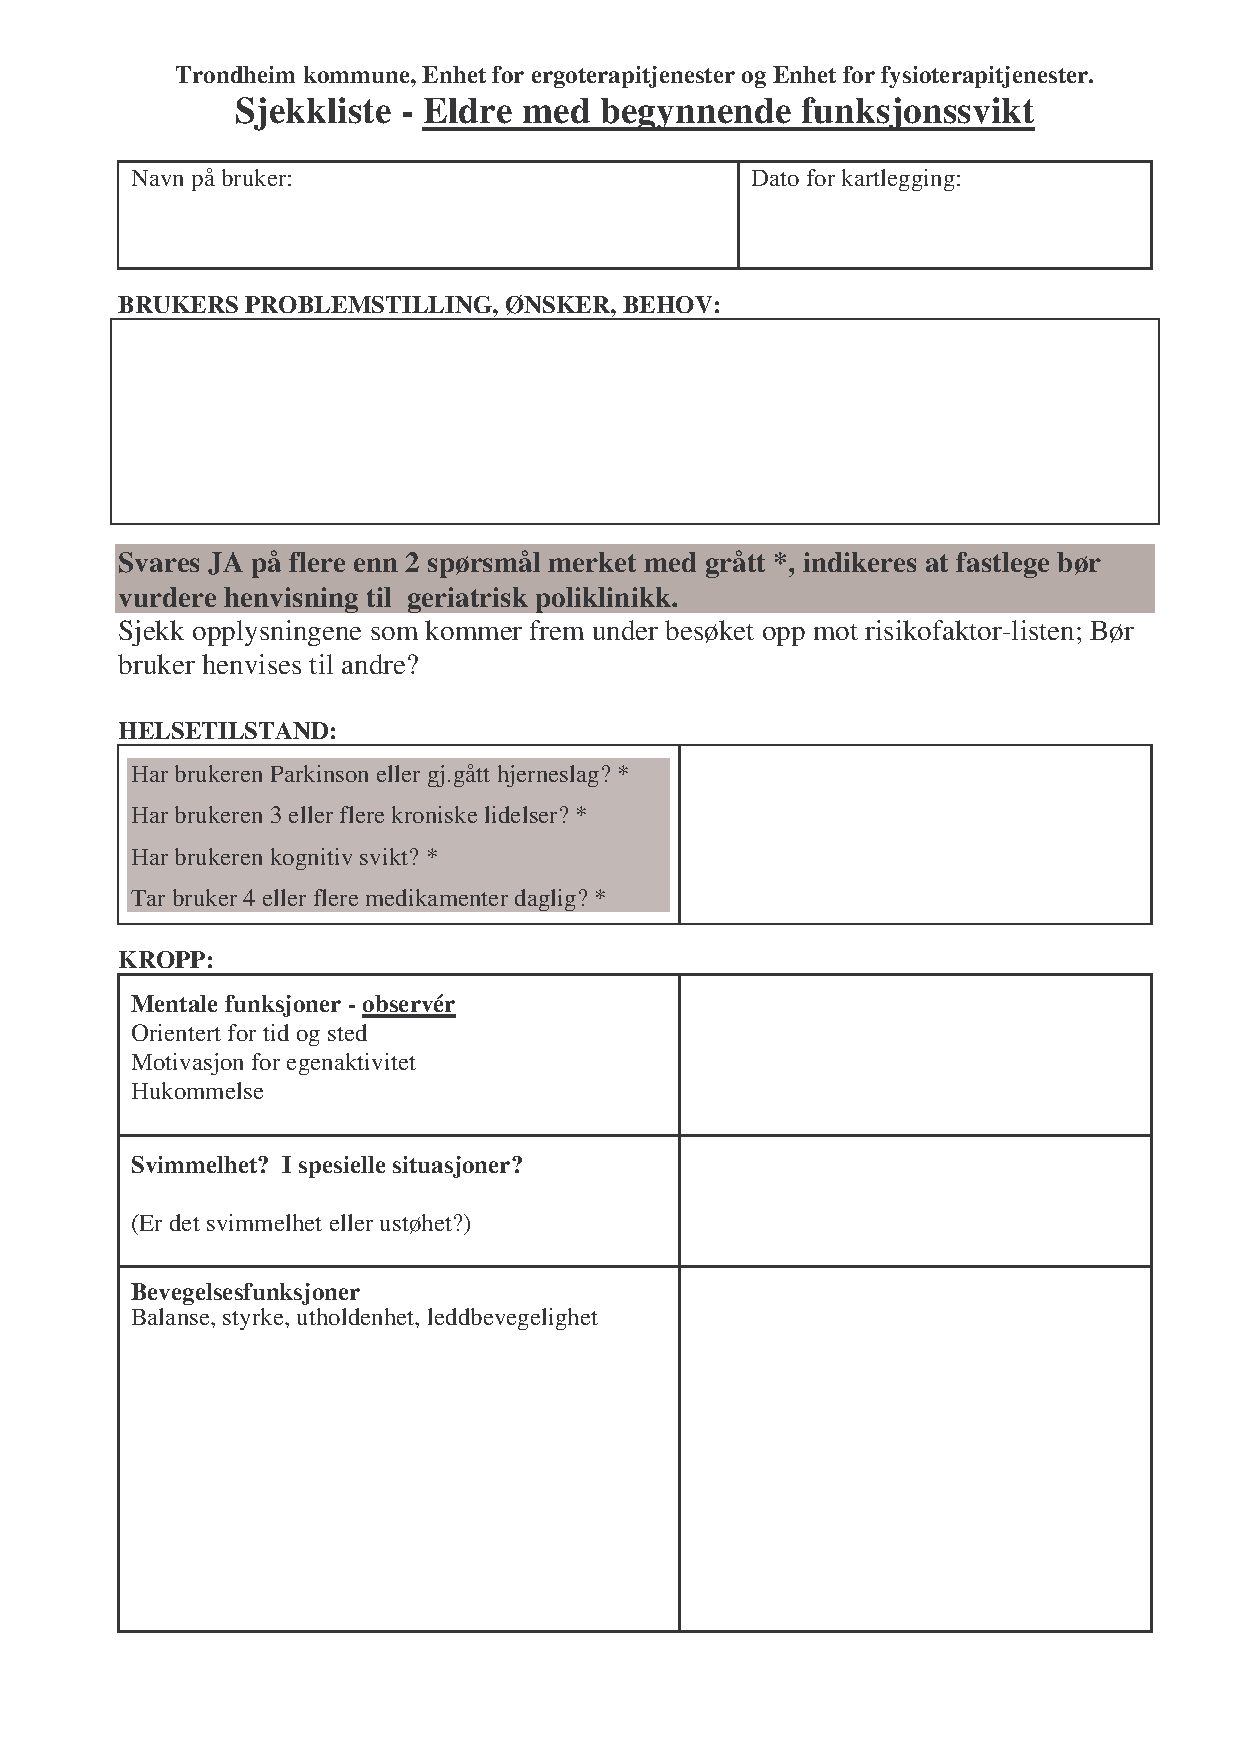
\includepdf[pages=-,scale=.8,pagecommand={\thispagestyle{plain}}]{checklist.pdf}
\chapter{Prototype 1 Visualizations}
\label{prototype1Viz}

\begin{figure}[h!]
\centering
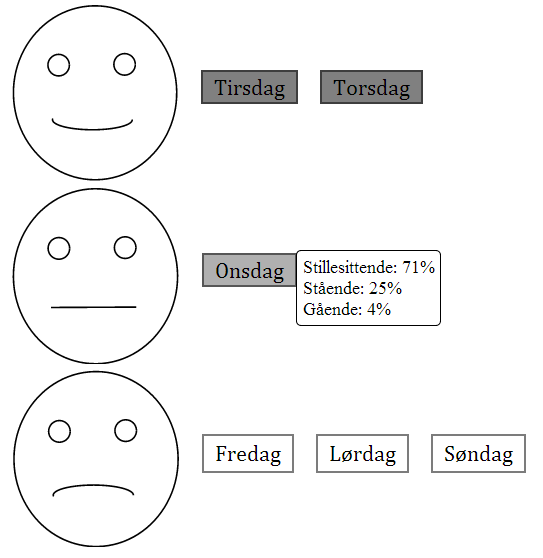
\includegraphics[totalheight=0.5\textheight, angle=-90]{u1First.png}
\caption[First version of U1]{First version of U1.}
\end{figure}

\begin{figure}[h!]
\centering
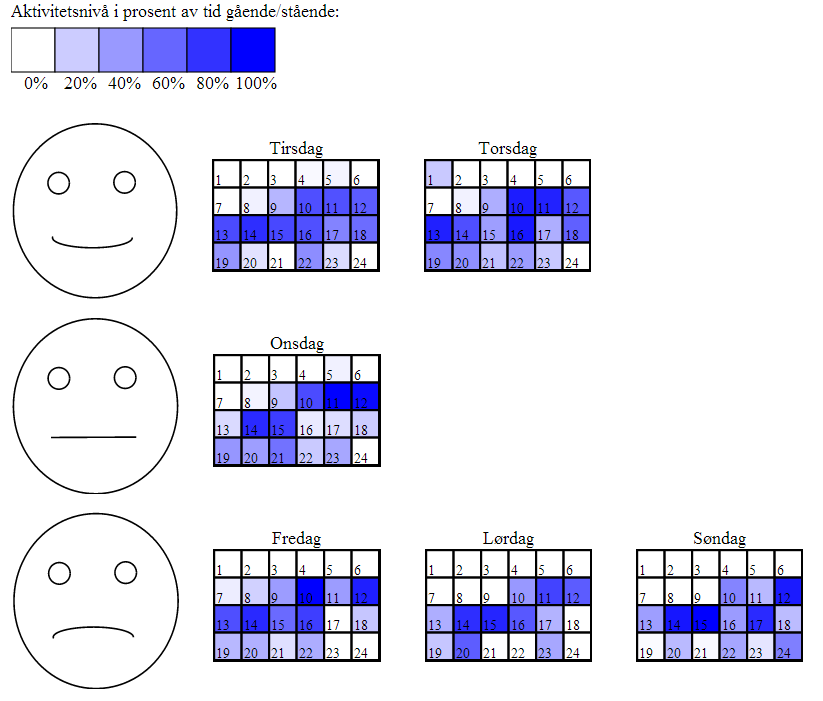
\includegraphics[totalheight=0.5\textheight, angle=90]{u2First.png}
\caption[First version of U2]{First version of U2.}
\end{figure}

\begin{figure}[h!]
\centering
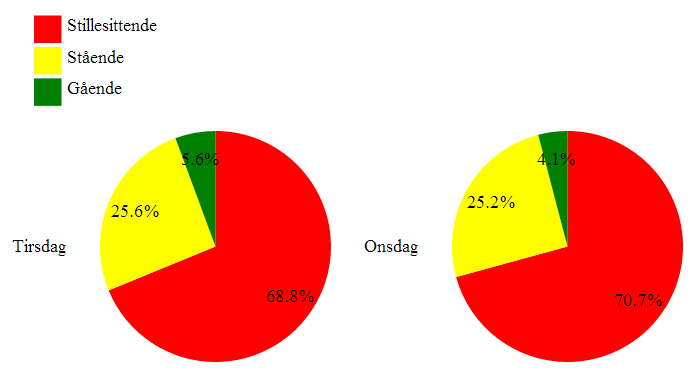
\includegraphics[totalheight=0.4\textheight, angle=-90]{f1First.png}
\caption[First version of F1]{First version of F1.}
\end{figure}

\begin{figure}[h!]
\centering
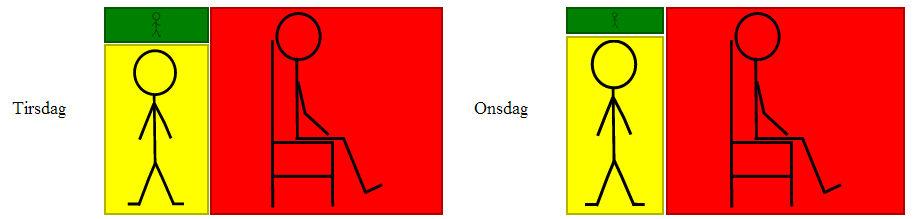
\includegraphics[totalheight=0.22\textheight, angle=90]{f2First.png}
\caption[First version of F2]{First version of F2.}
\end{figure}

\begin{figure}[h!]
\centering
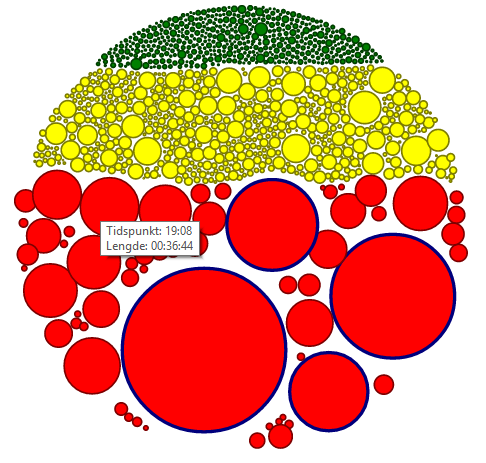
\includegraphics[totalheight=0.5\textheight, angle=-90]{f3First.png}
\caption[First version of F3]{First version of F3.}
\end{figure}

\begin{figure}[h!]
\centering
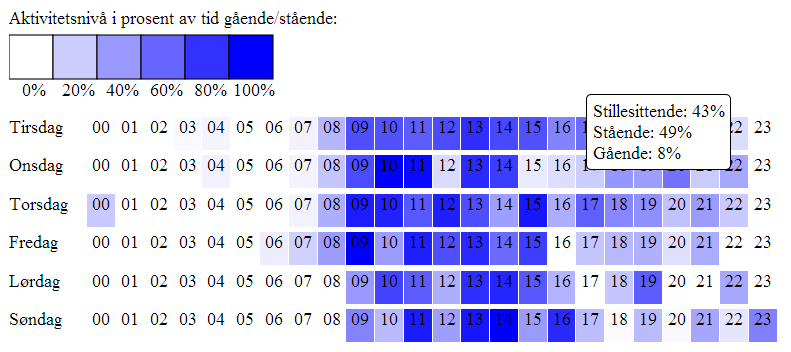
\includegraphics[totalheight=0.4\textheight, angle=90]{t1FirstWeek.png}
\caption[First version of T1]{First version of T1 in week overview.}
\end{figure}

\begin{figure}[h!]
\centering
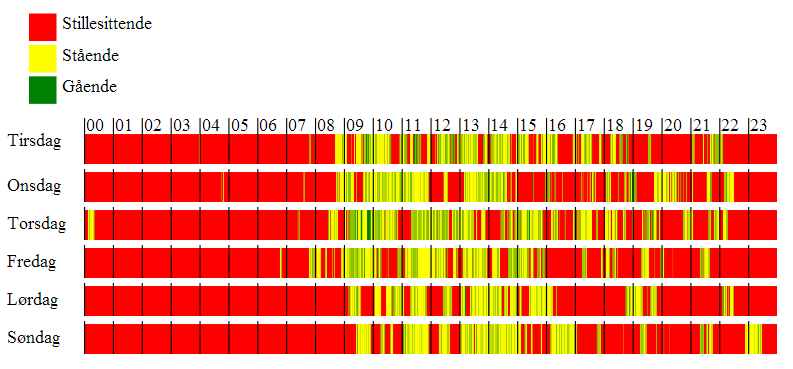
\includegraphics[totalheight=0.45\textheight, angle=-90]{t2FirstWeek.png}
\caption[First version of T2]{First version of T2 in week overview.}
\end{figure}

\begin{figure}[h!]
\centering
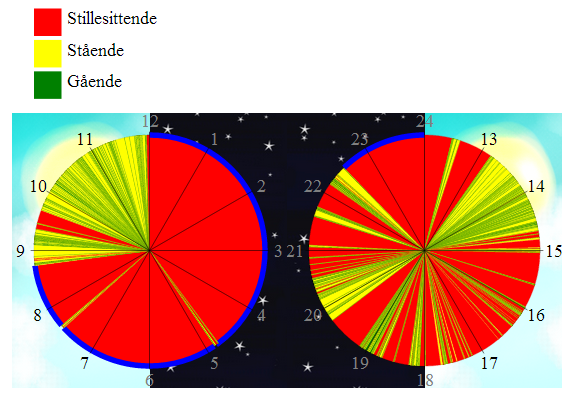
\includegraphics[totalheight=0.5\textheight, angle=90]{t3First.png}
\caption[First version of T3]{First version of T3}
\end{figure}

\begin{figure}[h!]
\centering
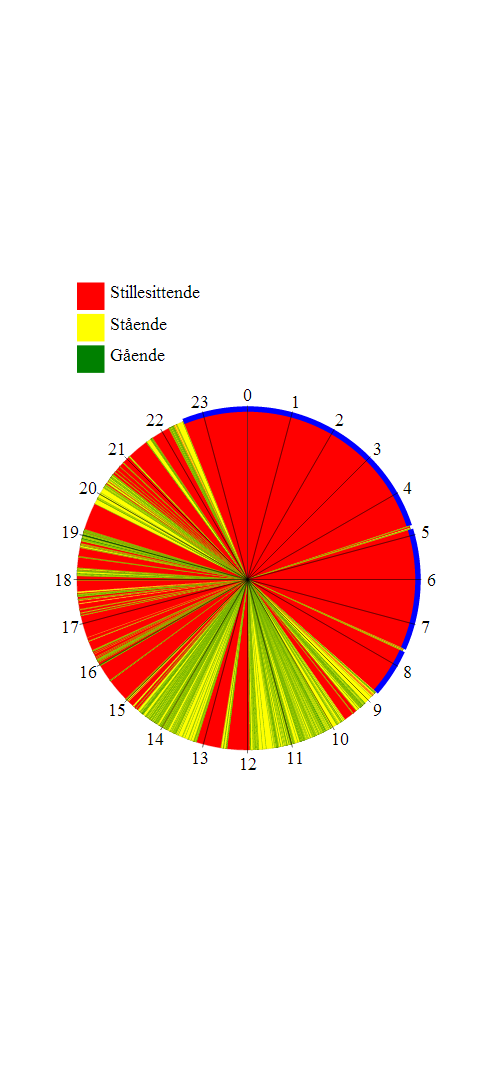
\includegraphics[totalheight=0.5\textheight, angle=-90]{t4First.png}
\caption[First version of T4]{First version of T4.}
\end{figure}


\chapter{Prototype 2 Visualizations}
\label{prototype2Viz}

\begin{figure}[h!]
\centering
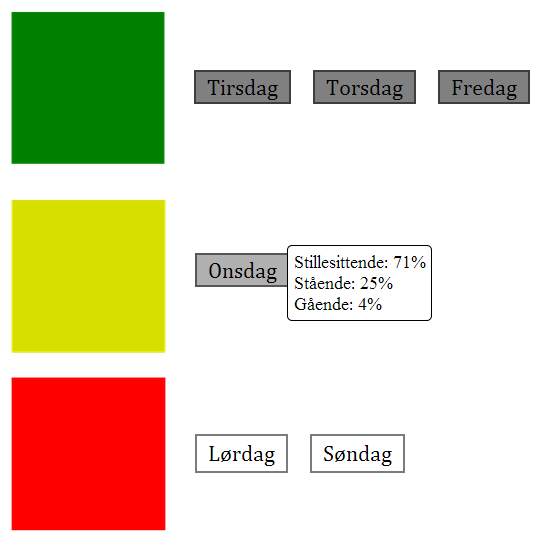
\includegraphics[totalheight=0.5\textheight, angle=-90]{u1Second.png}
\caption[Second version of U1]{Second version of U1.}
\end{figure}

\begin{figure}[h!]
\centering
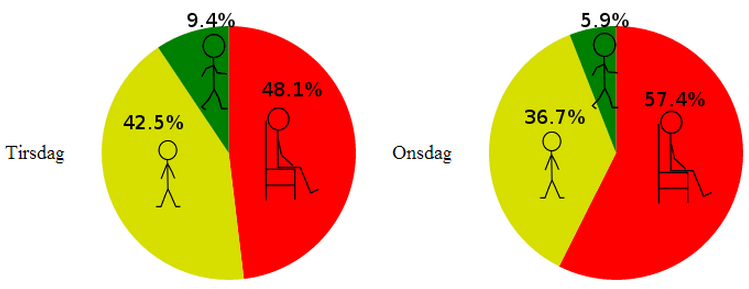
\includegraphics[totalheight=0.35\textheight, angle=90]{f1Second.png}
\caption[Second version of F1]{Second version of F1.}
\end{figure}

\begin{figure}[h!]
\centering
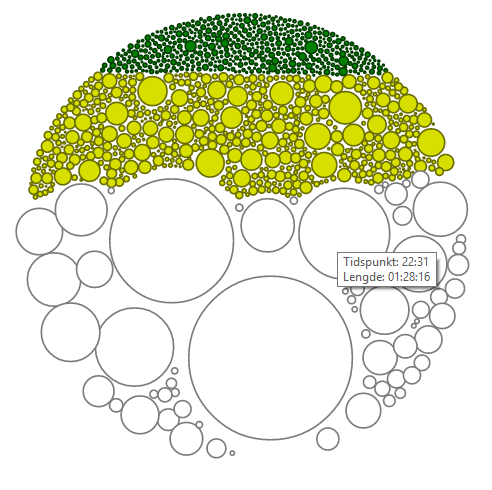
\includegraphics[totalheight=0.5\textheight, angle=-90]{f3Second.png}
\caption[Second version of F3]{Second version of F3.}
\end{figure}

\begin{figure}[h!]
\centering
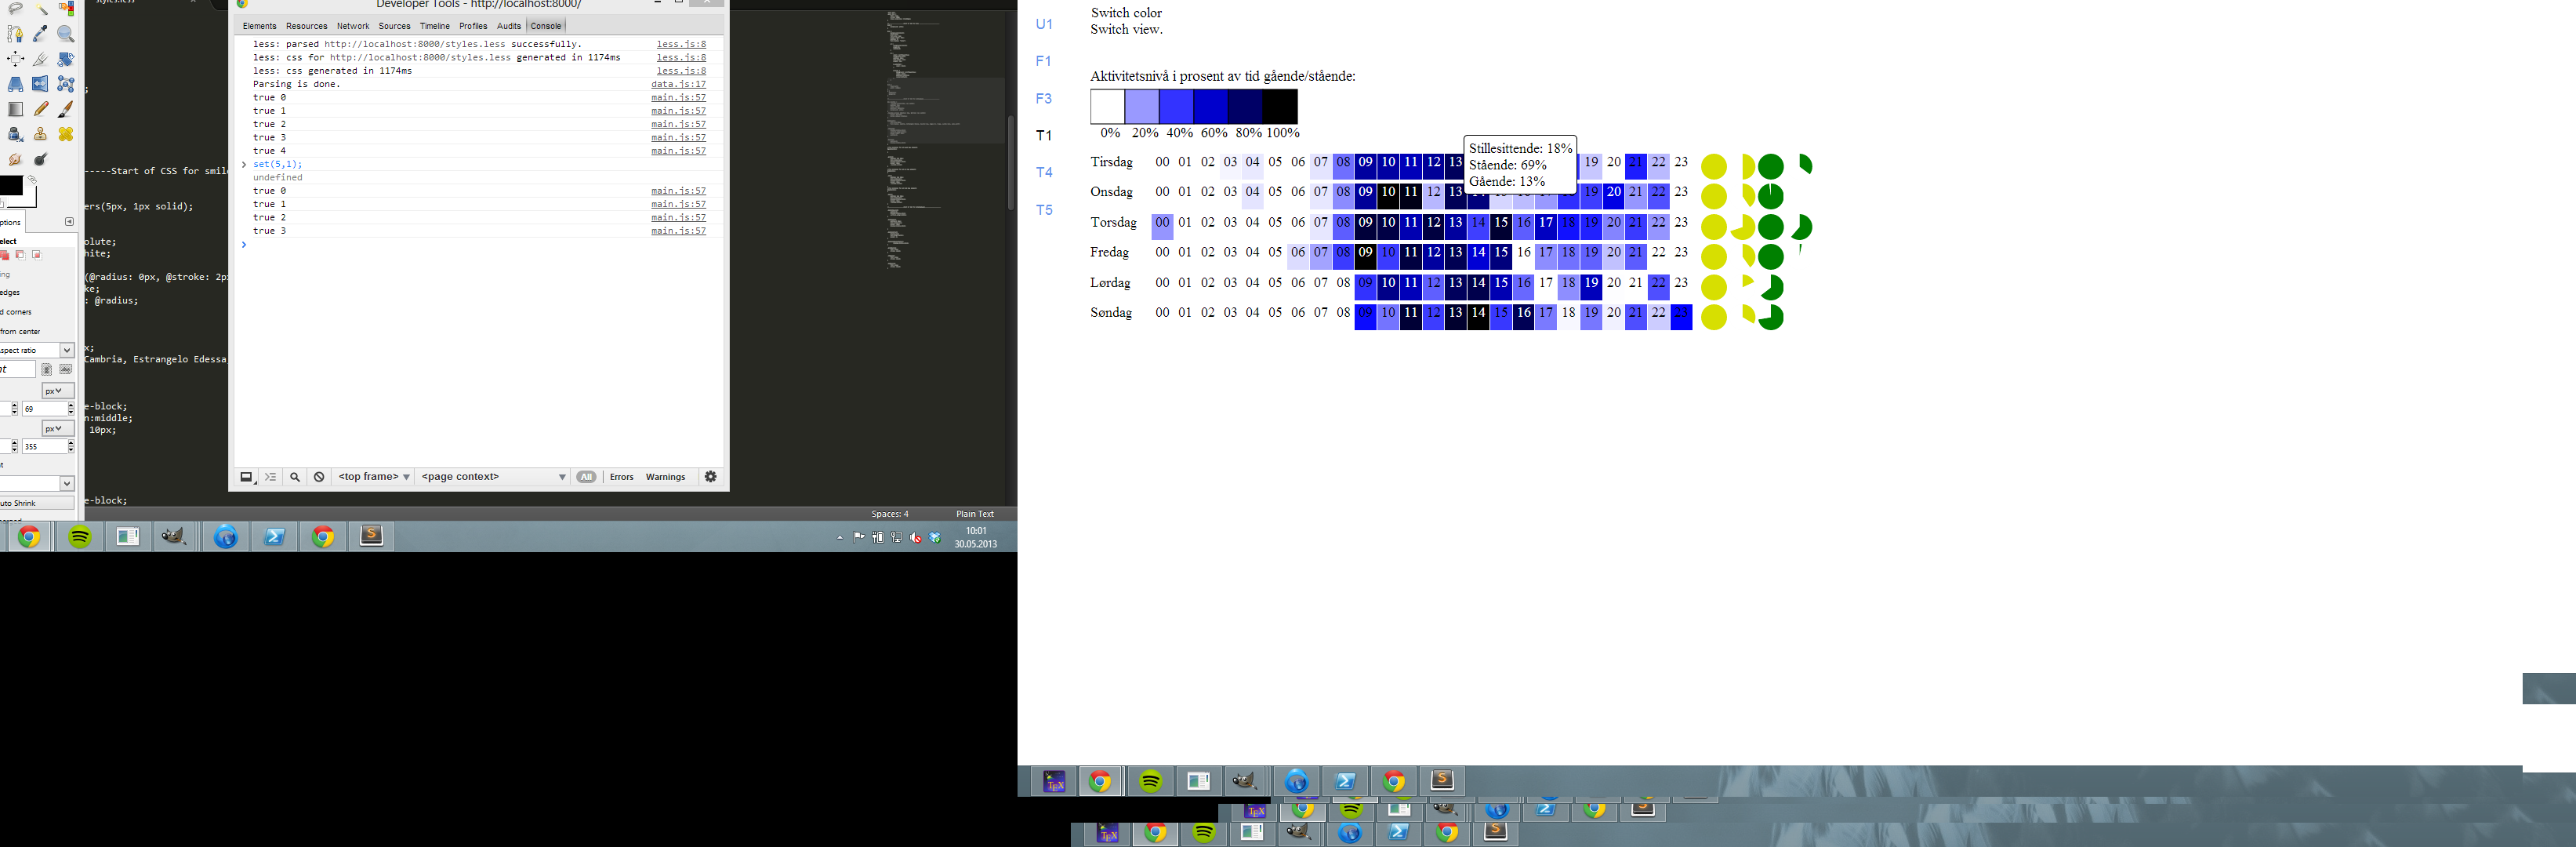
\includegraphics[totalheight=0.35\textheight, angle=90]{t1SecondWeek.png}
\caption[Second version of T1]{Second version of T1 in week overview.}
\end{figure}

\begin{figure}[h!]
\centering
\includegraphics[totalheight=0.5\textheight, angle=-90]{t4Second.png}
\caption[Second version of T4]{Second version of T4.}
\end{figure}

\begin{figure}[h!]
\centering
\includegraphics[totalheight=0.5\textheight, angle=90]{t5SecondWeek.png}
\caption[First version of T5]{First version of T5 in week overview.}
\end{figure}



\end{document} 
